\documentclass[11pt,a4paper]{article}
\usepackage{amsmath}
\usepackage{amsfonts}
\usepackage{amssymb}
\usepackage{amsthm}
\usepackage{graphicx}
\usepackage[margin=1in]{geometry}
\usepackage{hyperref}
\usepackage{listings}
\usepackage{xcolor}
\usepackage{algorithm}
\usepackage{algpseudocode}
\usepackage{cleveref}
\usepackage{caption}
\usepackage{subcaption}

% Theorem-like environments
\theoremstyle{plain}
\newtheorem{theorem}{Theorem}[section]
\newtheorem{lemma}[theorem]{Lemma}
\newtheorem{proposition}[theorem]{Proposition}
\newtheorem{corollary}[theorem]{Corollary}

\theoremstyle{definition}
\newtheorem{definition}[theorem]{Definition}
\newtheorem{assumption}[theorem]{Assumption}
\newtheorem{condition}[theorem]{Condition}
\newtheorem{example}[theorem]{Example}

\theoremstyle{remark}
\newtheorem{remark}[theorem]{Remark}
\newtheorem{note}[theorem]{Note}

% cleveref names for theorem-like environments
\crefname{theorem}{theorem}{theorems}
\Crefname{theorem}{Theorem}{Theorems}
\crefname{lemma}{lemma}{lemmas}
\Crefname{lemma}{Lemma}{Lemmas}
\crefname{proposition}{proposition}{propositions}
\Crefname{proposition}{Proposition}{Propositions}
\crefname{corollary}{corollary}{corollaries}
\Crefname{corollary}{Corollary}{Corollaries}
\crefname{definition}{definition}{definitions}
\Crefname{definition}{Definition}{Definitions}
\crefname{assumption}{assumption}{assumptions}
\Crefname{assumption}{Assumption}{Assumptions}
\crefname{condition}{condition}{conditions}
\Crefname{condition}{Condition}{Conditions}
\crefname{remark}{remark}{remarks}
\Crefname{remark}{Remark}{Remarks}
\crefname{example}{example}{examples}
\Crefname{example}{Example}{Examples}
\crefname{algorithm}{algorithm}{algorithms}
\Crefname{algorithm}{Algorithm}{Algorithms}

\usepackage[backend=biber,style=numeric,sorting=nty]{biblatex}
\addbibresource{ref.bib}

\title{Mesoscopic Model: Computational Framework for Dynamics Study}
\author{Research Project}
\date{\today}

\begin{document}

\maketitle

\tableofcontents
\newpage

% \section{Background}

% \subsection{Ising Models}

% The Ising model is a fundamental statistical mechanical model that describes the behavior of magnetic systems. For a two-dimensional square lattice with nearest-neighbor interactions, the Hamiltonian is given by:

% \begin{equation}
% 	H = -J \sum_{\langle i,j \rangle} \sigma_i \sigma_j - h \sum_i \sigma_i
% \end{equation}

% where $\sigma_i \in \{-1, +1\}$ are the spin variables, $J$ is the coupling strength, $h$ is the external magnetic field, and $\langle i,j \rangle$ denotes nearest-neighbor pairs.

% \subsubsection{Critical Temperature}

% The critical temperature $T_c$ is a fundamental parameter that determines the phase transition between ordered and disordered phases. We experimentally use $T_c = 1.0$ and $T_c = 4.0$.

% \begin{equation}
% 	T_c = \frac{2J}{k_B \ln(1 + \sqrt{2})} \approx \frac{2.269J}{k_B}
% \end{equation}

% where $k_B$ is the Boltzmann constant. This critical temperature separates two distinct phases:

% \begin{itemize}
% 	\item \textbf{High temperature regime} ($T > T_c$): The system is in a \textit{disordered phase} where spins are randomly oriented, resulting in zero net magnetization. The system exhibits thermal fluctuations and short-range correlations.

% 	\item \textbf{Low temperature regime} ($T < T_c$): The system is in an \textit{ordered phase} where spins tend to align, leading to non-zero magnetization. The system exhibits long-range order and reduced thermal fluctuations.

% 	\item \textbf{Critical region} ($T \approx T_c$): The system undergoes a phase transition with critical phenomena, including diverging correlation lengths and power-law scaling behavior.
% \end{itemize}

% The temperature ratio $T/T_c$ is a key parameter that determines the physical regime of the system. In our simulations, we often work in the high-temperature regime where $T/T_c > 1$, corresponding to the disordered phase.

% \subsubsection{Units and Normalization}

% In our computational framework, we use dimensionless units where the Boltzmann constant $k_B = 1$ and the coupling strength $J = 1$. This normalization simplifies the calculations while preserving the essential physics. The temperature $T$ is therefore dimensionless, and the critical temperature becomes:

% \begin{equation}
% 	T_c = \frac{2}{\ln(1 + \sqrt{2})} \approx 2.269
% \end{equation}

% This approach is common in computational statistical physics as it eliminates the need to track physical units while maintaining the correct scaling relationships between temperature, energy, and other thermodynamic quantities.

% In this normalization, the inverse temperature $\beta = 1/T$ is directly computed from the dimensionless temperature $T$. For example, with $T = 6.808$, we have $\beta = 1/6.808 \approx 0.147$, which represents the strength of thermal fluctuations in the system.

% \subsection{Nonlocal Interactions and Kac Potentials}

% The classical Ising model only considers nearest-neighbor interactions.
% However, many physical systems exhibit \emph{nonlocal interactions} that extend beyond immediate neighbors.
% To incorporate such effects, one introduces \emph{Kac-type potentials}, which are long-range interaction kernels that decay with distance.

% A Kac potential $J_\epsilon(x,y)$ is typically defined as a smooth, radially symmetric function that depends on a parameter $\epsilon > 0$ controlling the interaction range:
% \begin{equation}
% 	J_\epsilon(x, y) = \epsilon^{-d} J\left(\frac{|x - y|}{\epsilon}\right),
% \end{equation}
% where $J(r)$ is a normalized kernel function, and $d$ is the spatial dimension. Larger values of $\epsilon$ correspond to longer-range interactions, while smaller values approach the nearest-neighbor limit.

% A widely used example of a Kac potential is the Gaussian kernel:
% \begin{equation}\label{eq:J-Gaussian}
% 	J_\epsilon(x) \;=\; \frac{1}{(2\pi\epsilon^2)^{d/2}}
% 	\exp\!\left(-\frac{|x|^2}{2\epsilon^2}\right).
% \end{equation}

% The Ising Hamiltonian with Kac interactions is given by
% \begin{equation}\label{eq:H-Kac}
% 	H(\sigma) \;=\; -\frac{1}{2}\sum_{x,y} J_\epsilon(x,y)\,\sigma(x)\sigma(y) \;-\; h \sum_{x} \sigma(x).
% \end{equation}

% \subsection{Glauber Dynamics}
% \label{sec:glauber}
% To describe the stochastic time evolution of the spin system, we adopt \emph{Glauber dynamics}.
% At each site, spins flip randomly due to thermal fluctuations, with probabilities determined by the change in the Hamiltonian.

% \paragraph{Spin-Flip Probability.}
% Let $\beta > 0$ be the inverse temperature.
% For a given spin $\sigma(x)$, the probability of flipping at site $x$ depends on the local field
% \begin{equation}\label{eq:hloc}
% 	h_{\epsilon}(x) \;=\; h + \sum_{y\neq x} J_\epsilon(x-y)\,\sigma(y).
% \end{equation}
% The corresponding flip probability can be written in several equivalent forms:
% \begin{equation}\label{eq:flip-prob}
% 	\begin{split}
% 		P\big(\sigma(x)\!\to\!-\sigma(x)\big)
% 		 & = \frac{1}{1 + \exp\!\big(\beta \Delta H_x\big)}
% 		\quad \text{(from energy difference)}                                \\
% 		 & = \frac{1}{1 + \exp\!\big(2\beta\,\sigma(x) h_{\epsilon}(x)\big)}
% 		\quad \text{(logistic form)}                                         \\
% 		 & = \frac{\exp\!\big(-\beta\sigma(x) h_{\epsilon}(x)\big)}
% 		{2\cosh\!\big(\beta h_{\epsilon}(x)\big)}
% 		\quad \text{(factorized form, cf.~Masi et al.\cite{de1994glauber})}.
% 	\end{split}
% \end{equation}
% Here, $\Delta H_x = H(\sigma^x) - H(\sigma) = 2\sigma(x)h_\epsilon(x)$ denotes the energy change when flipping the spin at $x$.

% \paragraph{Initialization by Gaussian Random Field.}
% Let the lattice be a periodic $L\times L$ grid
% \begin{equation}
% 	\Lambda=\{(x_i,y_j):\ i,j=0,1,\dots,L-1\},\qquad (x_i=i,\ y_j=j).
% \end{equation}
% We will construct a zero-mean, stationary Gaussian random field (GRF)
% $\phi:\Lambda\to\mathbb{R}$ and then convert it to spins $\sigma_{i,j}\in\{-1,+1\}$. This initialization creates spatially correlated patterns with tunable length scales and contrast.

% A stationary GRF is fully characterized by either its covariance $C(\mathbf{r})$ or its
% power spectral density (PSD) $S(\mathbf{k})$, related by the Fourier transform:
% \begin{equation}
% 	S(\mathbf{k})=\sum_{\mathbf{r}\in\mathbb{Z}^2} C(\mathbf{r})\,e^{-i\,\mathbf{k}\cdot\mathbf{r}}\!,
% 	\qquad
% 	C(\mathbf{r})=\frac{1}{(2\pi)^2}\!\int_{[-\pi,\pi]^2} S(\mathbf{k})\,e^{i\,\mathbf{k}\cdot\mathbf{r}}\,d\mathbf{k}.
% \end{equation}

% Typical isotropic choices for $S(\mathbf{k})$ include the Gaussian spectrum
% $S(\mathbf{k})=\sigma^2\exp(-\tfrac{\ell^2}{2}\|\mathbf{k}\|^2)$ with correlation length $\ell$,
% the Matérn spectrum $S(\mathbf{k})\propto (\kappa^2+\|\mathbf{k}\|^2)^{-(\nu+1)}$ with smoothness $\nu$,
% and power-law forms $S(\mathbf{k})\propto \|\mathbf{k}\|^{-\alpha}$ for $\alpha>0$. Larger $\ell$ (or smaller $\alpha$) yields larger coherent blobs, while $\sigma^2$ controls the marginal variance.

% On the $L\times L$ periodic lattice, we use discrete wavevectors
% \begin{equation}
% 	k_x(n)=\tfrac{2\pi n}{L},\quad n=0,\dots,L-1,
% 	\qquad k_y(m)=\tfrac{2\pi m}{L},\quad m=0,\dots,L-1,
% \end{equation}
% and set $\mathbf{k}_{n,m}=(k_x(n),k_y(m))$ with $S_{n,m}:=S(\mathbf{k}_{n,m})$. We then construct Fourier coefficients $\widehat{\phi}_{n,m}$ such that
% \begin{equation}
% 	\widehat{\phi}_{n,m}\sim\mathcal{CN}(0,S_{n,m}),\quad\text{independently over $(n,m)$,}
% \end{equation}
% with Hermitian symmetry $\widehat{\phi}_{(L-n)\bmod L,(L-m)\bmod L}=\overline{\widehat{\phi}_{n,m}}$ to ensure a real field. In practice we set
% \begin{equation}
% 	\widehat{\phi}_{n,m}=\sqrt{\tfrac{S_{n,m}}{2}}\,(Z^{(1)}_{n,m}+i\,Z^{(2)}_{n,m}),\quad Z^{(1)}_{n,m},Z^{(2)}_{n,m}\overset{\text{i.i.d.}}{\sim}\mathcal{N}(0,1),
% \end{equation}
% and impose conjugacy for paired frequencies. On self-conjugate modes ($n\in\{0,L/2\}$ or $m\in\{0,L/2\}$ for even $L$), we set $\widehat{\phi}_{n,m}\in\mathbb{R}$ by taking $Z^{(2)}_{n,m}=0$.

% The GRF is obtained by inverse FFT:
% \begin{equation}
% 	\phi_{i,j}=\frac{1}{L^2}\sum_{n=0}^{L-1}\sum_{m=0}^{L-1}\widehat{\phi}_{n,m}\,\exp\!\Big(i(k_x(n)x_i+k_y(m)y_j)\Big),
% 	\qquad (i,j)\in\{0,\dots,L-1\}^2.
% \end{equation}
% Then $\phi$ is a zero-mean Gaussian random field with PSD approximately $S$. The variance of $\phi$ is
% \begin{equation}
% 	\mathrm{Var}[\phi_{i,j}]=\frac{1}{L^2}\sum_{n,m} S_{n,m},
% \end{equation}
% and one can rescale $\phi$ to achieve a target variance $\sigma_\star^2$. The generated filed $\phi$ is despicted in \cref{fig:grf}.
% \begin{figure}
% 	\centering
% 	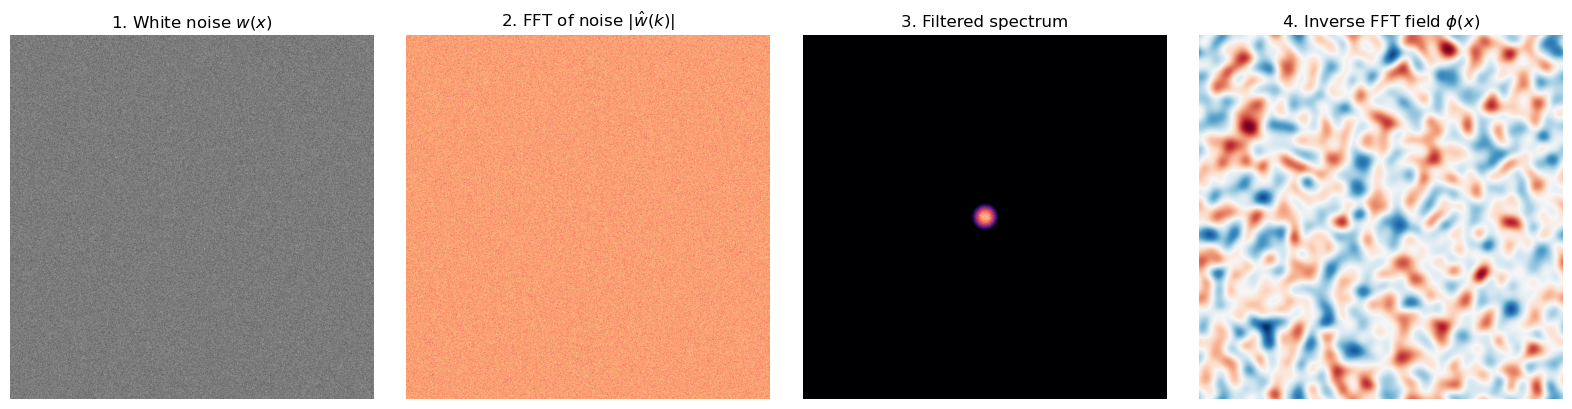
\includegraphics[width=0.8\textwidth]{fig/Gaussian_Random_Field.jpg}
% 	\caption{Example realization of a Gaussian random field.}
% 	\label{fig:grf}
% \end{figure}

% To map $\phi$ into a magnetization-like field $m\in[-1,1]$, one option is
% \begin{equation}
% 	m_{i,j}=m_0+(1-|m_0|)\,\tanh\!\Big(\tfrac{\phi_{i,j}}{\tau}\Big),
% \end{equation}
% where $m_0$ sets the mean magnetization and $\tau$ controls the nonlinearity, with smaller $\tau$ pushing values toward $\pm 1$. Alternatively, a linear clipping scheme may be used. Spins are then sampled independently with
% \begin{equation}
% 	\mathbb{P}(\sigma_{i,j}=+1)=\tfrac{1+m_{i,j}}{2},\qquad
% 	\mathbb{P}(\sigma_{i,j}=-1)=\tfrac{1-m_{i,j}}{2},
% \end{equation}
% yielding an Ising configuration $\sigma\in\{-1,+1\}^{L\times L}$.

% The parameter choices have direct impact on structure: the correlation length $\ell$ sets the typical blob size, the global mean $m_0$ fixes magnetization bias, and the field variance or $\tau$ controls contrast. The periodic construction is consistent with the lattice boundary conditions. An equivalent spatial view is to draw white noise $w_{i,j}\sim\mathcal{N}(0,1)$ and convolve with a filter whose Fourier response is $\sqrt{S(\mathbf{k})}$:
% \begin{equation}
% 	\phi \;\stackrel{d}{=}\; \mathcal{F}^{-1}\!\Big[\sqrt{S(\mathbf{k})}\,\mathcal{F}[w]\Big],
% \end{equation}
% which for Gaussian $S$ corresponds to a Gaussian blur (with periodic wrap) of white noise.

% \paragraph{Stochastic Simulation via Gillespie Algorithm.}
% The Glauber dynamics can be efficiently simulated using the Gillespie algorithm (\cref{alg:gillespie}),
% which generates statistically exact trajectories of continuous-time Markov processes.
% The procedure is:

% \begin{enumerate}
% 	\item Compute the total flip rate
% 	      \begin{equation}
% 		      R = \sum_{x} P\big(\sigma(x)\!\to\!-\sigma(x)\big).
% 	      \end{equation}
% 	\item Draw the next time increment $\Delta t$ from an exponential distribution with mean $1/R$.
% 	\item Select a site $x$ to flip with probability proportional to its individual rate.
% 	\item Update $\sigma(x)\mapsto -\sigma(x)$, recompute local fields if needed, and repeat.
% \end{enumerate}

% \begin{algorithm}[h!]
% 	\caption{Gillespie Simulation of Glauber Dynamics}
% 	\label{alg:gillespie}
% 	\begin{algorithmic}[1]
% 		\State Initialize spin configuration $\sigma$ and compute local fields $h_\epsilon(x)$.
% 		\While{simulation time $t < t_{\mathrm{end}}$}
% 		\State Compute total flip rate
% 		\[
% 			R = \sum_{x} P\big(\sigma(x)\!\to\!-\sigma(x)\big).
% 		\]
% 		\State Sample time increment $\Delta t \sim \mathrm{Exp}(R)$.
% 		\State Select site $x$ with probability
% 		\[
% 			\frac{P(\sigma(x)\!\to\!-\sigma(x))}{R}.
% 		\]
% 		\State Flip spin: $\sigma(x) \gets -\sigma(x)$.
% 		\State Update local fields $h_\epsilon(y)$ if needed.
% 		\State Advance time: $t \gets t + \Delta t$.
% 		\EndWhile
% 	\end{algorithmic}
% \end{algorithm}
% This algorithm gives an implementation of the Gillespie method for Glauber dynamics, ensuring accurate simulation of the spin system's stochastic behavior.

% \paragraph{Stochastic Simulation via $\tau$-leaping Approximation.} The Gillespie algorithm simulates one event at a time, which can be slow for large systems.
% The \emph{$\tau$-leaping} method accelerates the simulation by leaping over a fixed time step $\tau$.
% During this interval, event rates are assumed to be constant.
% The number of events at each site is then sampled from a Poisson distribution.
% This allows many events to be processed in parallel.

% \begin{algorithm}[h]
% 	\caption{$\tau$-leaping for Glauber dynamics}
% 	\label{alg:tau-leaping}
% 	\begin{algorithmic}[1]
% 		\State Initialize spins $s$, time $t=0$
% 		\While{$t < T_{\text{end}}$}
% 		\State Compute local field $h_{\text{loc}}$
% 		\State Compute flip rates $r_i = \frac{1}{1 + \exp(2 \beta h_{\text{loc},i} s_i)}$
% 		\State Choose $\tau = \hat{\tau} / \max_i r_i$
% 		\State Sample $K_i \sim \mathrm{Poisson}(r_i \tau)$
% 		\State Update spins: if $K_i$ is odd, flip $s_i$
% 		\State $t \gets t + \tau$
% 		\EndWhile
% 	\end{algorithmic}
% \end{algorithm}

% \paragraph{Comparison of Gillespie and $\tau$-leaping} We compare the two methods within a small lattice ($L=128$) to validate the $\tau$-leaping approximation.
% We use the same initial conditions and parameters (temperature $T = 1.0$, coupling strength $J = 1.0$, and external field $h = 0.0$) for both simulations, and for each method, we run 20 independent trials to account for stochastic variability.
% The results are depicted in \cref{fig:gillespie_vs_tau_leaping}.
% The top left panel shows the averaged magnetization over time, while the top right panel displays the free energy evolution. The bottom panels illustrate the error between the two methods in terms of magnetization and free energy.
% The results demonstrate the mean energy and magnetization from both methods are in good agreement, and the varience of $\tau$-leaping is slightly larger than Gillespie.
% These findings confirm that the $\tau$-leaping method is a valid approximation for simulating Glauber dynamics, providing significant computational speedup (see \cref{tab:gillespie_vs_tau_leaping}) while maintaining accuracy with a small sacrifice in variation.
% \begin{figure}
% 	\centering
% 	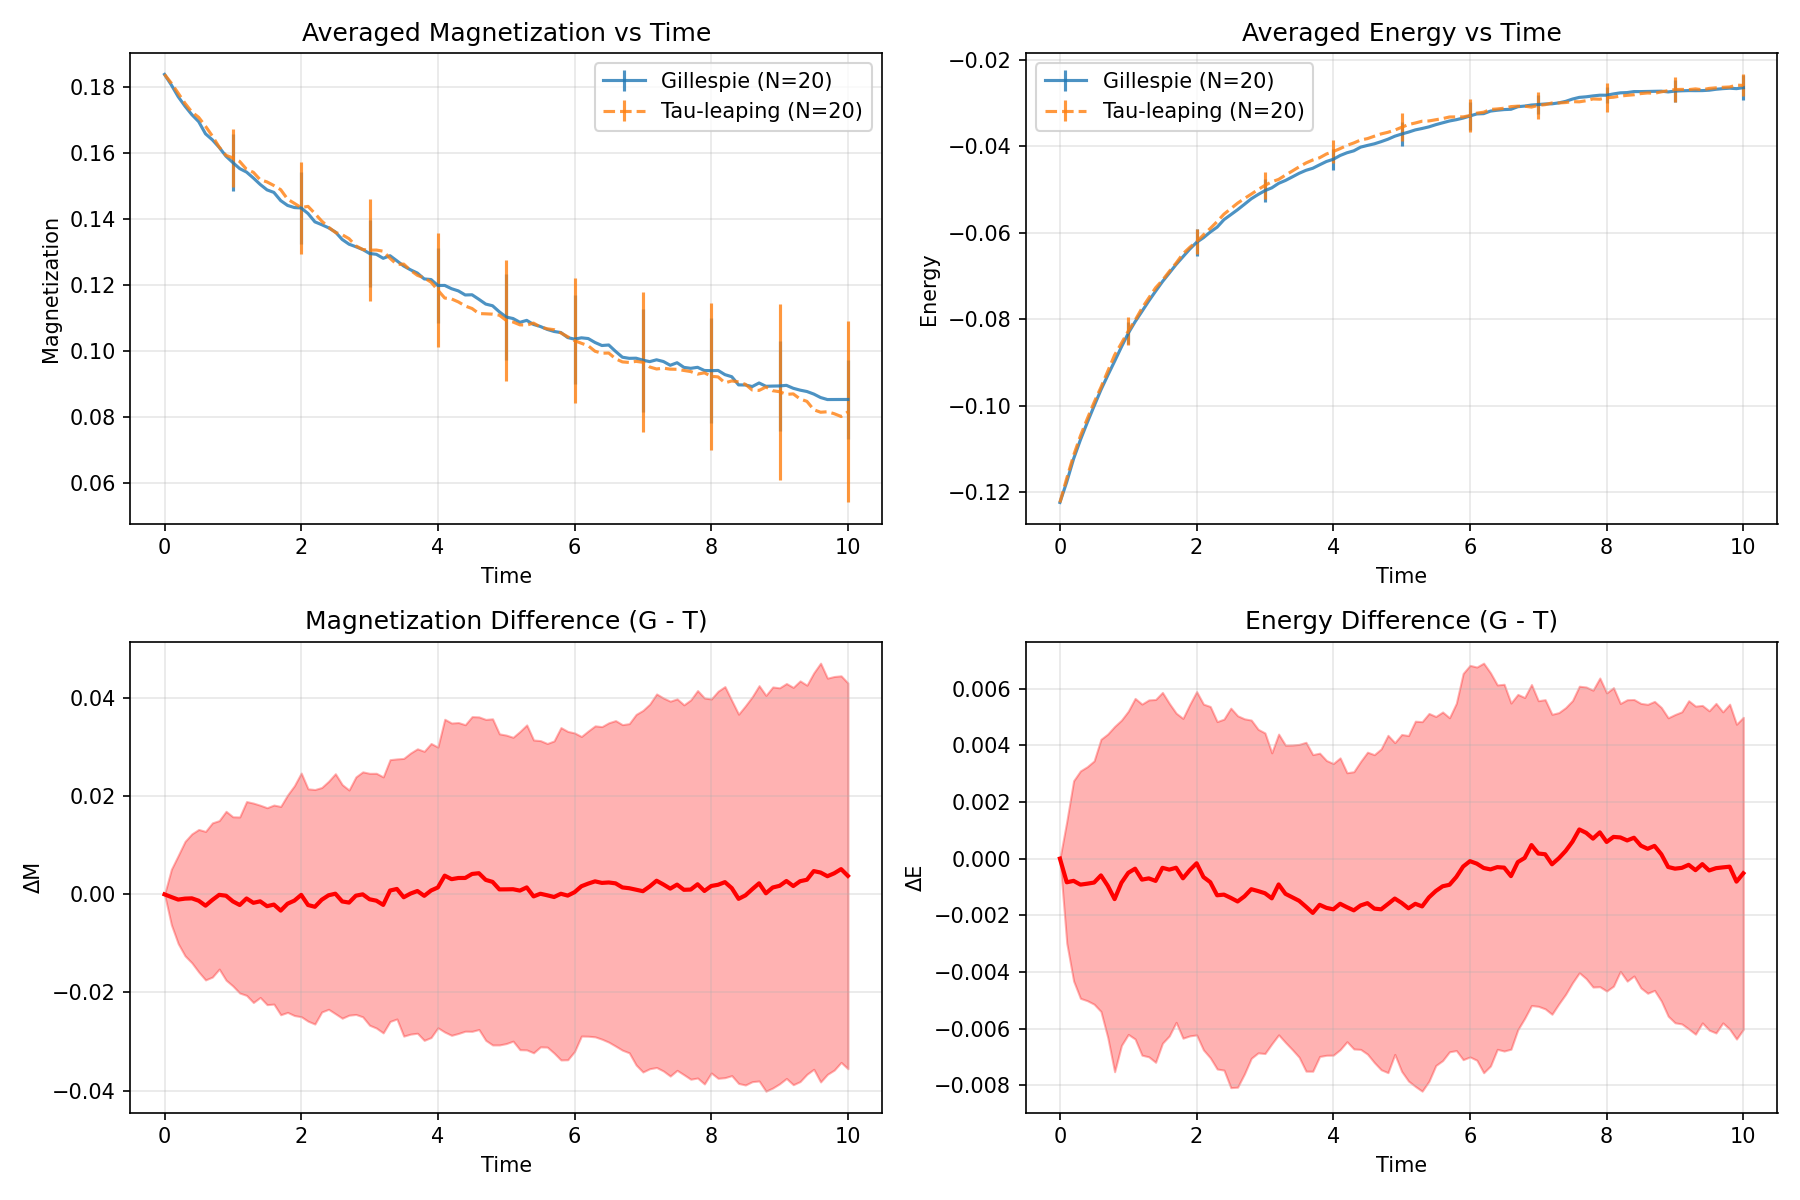
\includegraphics[width=0.8\textwidth]{fig/ising_L128_ell8.0_sigma1.0_tau1.0_m00.2_beta1.0_eps0.02_compare_N20.png}
% 	\caption{Comparison of Gillespie and $\tau$-leaping methods for simulating Glauber dynamics on a $128 \times 128$ lattice. The top left panel shows the averaged magnization over time and the top right panel shows the free energy evolution over time. The bottom panels show the error between the two methods in terms of magnetization and free energy.}
% 	\label{fig:gillespie_vs_tau_leaping}
% \end{figure}

% \begin{table}
% 	\centering
% 	\begin{tabular}{ll}
% 		\hline
% 		\hline
% 		Method         & Simulation Time (20 Trails) \\
% 		\hline
% 		Gillespie      & $786.51$s                   \\
% 		$\tau$-leaping & $10.79$s                    \\
% 		\hline
% 		\hline
% 	\end{tabular}
% 	\caption{Comparison of Gillespie and $\tau$-leaping methods for simulating Glauber dynamics on a $128 \times 128$ lattice. The table shows the final magnetization, free energy, and error for both methods.}
% 	\label{tab:gillespie_vs_tau_leaping}
% \end{table}

% \section{PDE}

% \subsection{Hydrodynamic Limit for Glauber-Kac}
% \label{subsec:hydro}
% Starting from the Glauber dynamics introduced in \cref{sec:glauber}, we consider the lattice in $[0,1]^d$. When the lattice size tends to infinity $L\to\infty$, and the empirical magnetization field
% \begin{equation}
% 	m^L(t,\mathbf{x}) = \frac{1}{B^d}\sum_{z\in \Lambda_B(\mathbf{x})} \sigma_t(z)
% \end{equation}
% is coarse-grained over mesoscopic blocks of size $B$, the law of large numbers implies convergence of $m^L(t,\mathbf{x})$ to a deterministic limit $m(t,\mathbf{x})$.
% In this hydrodynamic limit, the Glauber dynamics is described by the nonlinear nonlocal PDE
% \begin{equation}\label{eq:nonlocal}
% 	\partial_t m(t,\mathbf{x}) \;=\; -\,m(t,\mathbf{x})\;+\;\tanh\!\Big(\beta\, (J_\epsilon * m)(t,\mathbf{x}) + \beta h\Big),
% 	\qquad m(0,\mathbf{x})=m_0(\mathbf{x}),
% \end{equation}
% where the convolution operator is defined by
% \begin{equation}
% 	\label{eq:convolution}
% 	(J_\epsilon * m)(\mathbf{x}) \;=\; \int_{\mathbb{T}^d} J_\epsilon(\mathbf{x},\mathbf{y})\,m(\mathbf{y})\,d\mathbf{y}.
% \end{equation}

% Equation~\eqref{eq:nonlocal} is the mesoscopic limit of the Glauber--Kac dynamics:
% the microscopic randomness averages out, and the macroscopic magnetization evolves deterministically according to a nonlocal reaction term given by the Kac potential.

% \subsection{From the Nonlocal to the Local PDE}\paragraph{Step 1: Convolution expansion.}
% Assume the rescaled kernel $J_\epsilon(x) = \epsilon^{-d} J(x/\epsilon)$ with $\int_{\mathbb{R}^d} J(z)\,dz = 1$, $J$ even, and finite second moment
% \begin{equation}
% 	m_2 = \int_{\mathbb{R}^d} |z|^2 J(z)\,dz.
% \end{equation}

% Then
% \begin{equation}
% 	(J_\epsilon * m)(x) = \int_{\mathbb{R}^d} J(z)\, m(x+\epsilon z)\,dz.
% \end{equation}
% Expanding $m(x+\epsilon z)$ in Taylor series:
% \begin{equation}
% 	m(x+\epsilon z) = m(x) + \epsilon\, z\cdot \nabla m(x)
% 	+ \frac{\epsilon^2}{2}\, z^\top \nabla^2 m(x)\, z + O(\epsilon^3).
% \end{equation}

% By symmetry $\int J(z)\,z\,dz = 0$ and isotropy
% $\int J(z)\, z_i z_j\,dz = \frac{m_2}{d}\delta_{ij}$, we obtain
% \begin{equation}
% 	(J_\epsilon * m)(x) = m(x) + \frac{\epsilon^2 m_2}{2d}\,\Delta m(x) + O(\epsilon^4).
% \end{equation}
% Here, $m_2$ is the second moment of $J$.

% Define $\varepsilon_\epsilon = \frac{\epsilon^2 m_2}{2d}$, we have the local PDE approximation
% \begin{equation}
% 	\label{eq:local_tanh}
% 	\frac{\partial m}{\partial t} = -\,m + \tanh\!\Big(\beta\big(m + \varepsilon_\epsilon \Delta m + h\big)\Big).
% \end{equation}

% \paragraph{Step 2: Expansion of $\tanh$.}
% The nonlocal dynamics reads
% \begin{equation}
% 	\partial_t m = -\,m + \tanh\!\Big(\beta\big((J_\epsilon * m)(x) + h\big)\Big).
% \end{equation}
% Using Step~1,
% \begin{equation}
% 	\beta\big((J_\epsilon*m)(x) + h\big) = a + \delta + O(\epsilon^4),
% 	\quad a = \beta(m+h), \quad \delta = \beta \varepsilon_\epsilon \Delta m.
% \end{equation}
% Expanding $\tanh$ around $a$:
% \begin{equation}
% 	\tanh(a+\delta)
% 	= \tanh(a) + \text{sech}^2(a)\,\delta + O(\delta^2).
% \end{equation}
% Thus,
% \begin{equation}
% 	\tanh\!\Big(\beta((J_\epsilon*m)(x) + h)\Big)
% 	= \tanh\!\big(\beta(m+h)\big)
% 	+ \beta \varepsilon_\epsilon \text{sech}^2\!\big(\beta(m+h)\big)\,\Delta m
% 	+ O(\epsilon^4).
% \end{equation}
% For small $m,h$, expand
% \begin{equation}
% 	\begin{split}
% 		\tanh\!\big(\beta(m+h)\big)
% 		 & = \beta(m+h) - \frac{\beta^3}{3}(m+h)^3 + O(|m+h|^5), \\
% 		\text{sech}^2\!\big(\beta(m+h)\big)
% 		 & = 1 - \beta^2(m+h)^2 + O(|m+h|^4).
% 	\end{split}
% \end{equation}

% \paragraph{Resulting local PDE.}
% Keeping terms up to cubic order in $m,h$ and $O(\epsilon^2)$ in diffusion gives
% \begin{equation}
% 	\begin{split}
% 		\label{eq:local}
% 		\partial_t m
% 		 & = \kappa\, \Delta m
% 		+ (\beta - 1)\, m - \frac{\beta^3}{3}\, m^3 + \beta h
% 		- \beta^3(m^2 h + m h^2) - \frac{\beta^3}{3} h^3
% 		+ O(\epsilon^4, |m|^5, |h|^5), \\
% 		 & = \kappa\, \Delta m
% 	\end{split}
% \end{equation}
% with the effective diffusion coefficient
% \begin{equation}
% 	\kappa = \beta \varepsilon_\epsilon = \beta\, \frac{m_2}{2d}\, \epsilon^2.
% \end{equation}


% \paragraph{Allen-Cahn form.}
% As a simplified model, we consider the Allen-Cahn equation:
% \begin{equation}
% 	\label{eq:allen-cahn}
% 	\partial_t m = \kappa\, \Delta m - f(m) + \beta h,
% 	\qquad
% 	f(m) = r m + u m^3,
% \end{equation}
% with parameters
% \begin{equation}
% 	r = 1-\beta,
% 	\qquad u = \frac{\beta^3}{3}.
% \end{equation}



% \section{Experimental Settings}

% \subsection{Parameter Configuration}

% Our computational experiments are designed to systematically explore the parameter space of the Ising model and its mesoscopic approximations. The base configuration uses:

% \begin{itemize}
% 	\item \textbf{Coupling strength}: $J = 1.0$ (dimensionless units)
% 	\item \textbf{Critical temperature}: $T_c = 2.27$ (for 2D square lattice)
% 	\item \textbf{Lattice size}: $L = 1024, 2048$ with coarse-graining to $M = 128$
% 	\item \textbf{Block size}: $B = 8, 16$ (coarse-graining ratio $L/M = 8$)
% 	\item \textbf{Spatial resolution}: $\delta = 1/M = 0.0078125$
% \end{itemize}

% \subsubsection{Temperature Regimes}

% We investigate two distinct temperature regimes:

% \begin{enumerate}
% 	\item \textbf{Low temperature} ($T = 1.0$): Below critical temperature, corresponding to the ordered phase where $T/T_c \approx 0.44$
% 	\item \textbf{High temperature} ($T = 4.0$): Above critical temperature, corresponding to the disordered phase where $T/T_c \approx 1.76$
% \end{enumerate}

% \subsubsection{External Field Variations}

% The external magnetic field $h$ is varied across four values to study its effect on the system dynamics:

% \begin{itemize}
% 	\item $h = 0.0$ (no external field)
% 	      % \item $h = 0.5$ (weak external field)
% 	\item $h = 1.0$ (moderate external field)
% 	      % \item $h = 2.0$ (strong external field)
% \end{itemize}

% \subsubsection{Kernel Range Studies}

% To investigate the role of interaction range in nonlocal dynamics, we vary the kernel domain size:

% \begin{itemize}
% 	\item \textbf{Local interactions}: $\epsilon \to 0$ (nearest-neighbor only)
% 	\item \textbf{Short-range nonlocal}: $\epsilon = 2\delta$ (extended local interactions)
% 	\item \textbf{Medium-range nonlocal}: $\epsilon = 4\delta$ (moderate nonlocal interactions)
% 	\item \textbf{Long-range nonlocal}: $\epsilon = 8\delta$ (strong nonlocal interactions)
% \end{itemize}

% This systematic variation allows us to study the transition from local to nonlocal behavior and its impact on pattern formation and dynamics.

% This computational framework will provide insights into:

% \begin{itemize}
% 	\item The relationship between microscopic and macroscopic dynamics
% 	\item The validity of continuum approximations
% 	\item The role of nonlocal interactions in pattern formation
% 	\item Machine learning approaches for complex dynamics
% \end{itemize}

% \subsection{Data v.s. PDE Solutions}
% \begin{table}[h]
% 	\centering
% 	\begin{tabular}{lllll}
% 		\hline
% 		\hline
% 		\textbf{External field $h$} & \textbf{Temperature $T$} & \textbf{Kernel parameter $\epsilon$} & \textbf{Lattice size $L$} & \textbf{Results}                                  \\
% 		\hline
% 		0                           & 1                        & 0.015625                             & 1024                      & \Cref{fig:pde_comparison_h0_T1_eps0.015625}       \\
% 		0                           & 4                        & 0.015625                             & 1024                      & \Cref{fig:pde_comparison_h0_T4_eps0.015625}       \\
% 		1                           & 1                        & 0.015625                             & 1024                      & \Cref{fig:pde_comparison_h1_T1_eps0.015625}       \\
% 		1                           & 4                        & 0.015625                             & 1024                      & \Cref{fig:pde_comparison_h1_T4_eps0.015625}       \\
% 		0                           & 1                        & 0.03125                              & 1024                      & \Cref{fig:pde_comparison_h0_T1_eps0.03125}        \\
% 		0                           & 4                        & 0.03125                              & 1024                      & \Cref{fig:pde_comparison_h0_T4_eps0.03125}        \\
% 		1                           & 1                        & 0.03125                              & 1024                      & \Cref{fig:pde_comparison_h1_T1_eps0.03125}        \\
% 		1                           & 4                        & 0.03125                              & 1024                      & \Cref{fig:pde_comparison_h1_T4_eps0.03125}        \\
% 		0                           & 1                        & 0.0625                               & 1024                      & \Cref{fig:pde_comparison_h0_T1_eps0.0625}         \\
% 		0                           & 4                        & 0.0625                               & 1024                      & \Cref{fig:pde_comparison_h0_T4_eps0.0625}         \\
% 		1                           & 1                        & 0.0625                               & 1024                      & \Cref{fig:pde_comparison_h1_T1_eps0.0625}         \\
% 		1                           & 4                        & 0.0625                               & 1024                      & \Cref{fig:pde_comparison_h1_T4_eps0.0625}         \\
% 		0                           & 1                        & 0.015625                             & 2048                      & \Cref{fig:pde_comparison_h0_T1_eps0.015625_L2048} \\
% 		0                           & 4                        & 0.015625                             & 2048                      & \Cref{fig:pde_comparison_h0_T4_eps0.015625_L2048} \\
% 		1                           & 1                        & 0.015625                             & 2048                      & \Cref{fig:pde_comparison_h1_T1_eps0.015625_L2048} \\
% 		1                           & 4                        & 0.015625                             & 2048                      & \Cref{fig:pde_comparison_h1_T4_eps0.015625_L2048} \\
% 		0                           & 1                        & 0.03125                              & 2048                      & \Cref{fig:pde_comparison_h0_T1_eps0.03125_L2048}  \\
% 		0                           & 4                        & 0.03125                              & 2048                      & \Cref{fig:pde_comparison_h0_T4_eps0.03125_L2048}  \\
% 		1                           & 1                        & 0.03125                              & 2048                      & \Cref{fig:pde_comparison_h1_T1_eps0.03125_L2048}  \\
% 		1                           & 4                        & 0.03125                              & 2048                      & \Cref{fig:pde_comparison_h1_T4_eps0.03125_L2048}  \\
% 		0                           & 1                        & 0.0625                               & 2048                      & \Cref{fig:pde_comparison_h0_T1_eps0.0625_L2048}   \\
% 		0                           & 4                        & 0.0625                               & 2048                      & \Cref{fig:pde_comparison_h0_T4_eps0.0625_L2048}   \\
% 		1                           & 1                        & 0.0625                               & 2048                      & \Cref{fig:pde_comparison_h1_T1_eps0.0625_L2048}   \\
% 		1                           & 4                        & 0.0625                               & 2048                      & \Cref{fig:pde_comparison_h1_T4_eps0.0625_L2048}   \\
% 		\hline
% 		\hline
% 	\end{tabular}
% 	\caption{Comparison of original data and PDE solutions under different external field $h$, temperature $T$, and kernel parameter $\epsilon$.}
% 	\label{tab:pde_comparison}
% \end{table}

% The results are presented in \Cref{tab:pde_comparison}.
% We compare the results from microscopic simulations (\Cref{alg:tau-leaping}) with the solutions of the nonlocal PDE (\cref{eq:nonlocal}) and the local PDE with $\tanh$ form (\cref{eq:local_tanh}) and the Allen-Cahn equation (\cref{eq:allen-cahn}) from $t=0$ to $t=20$, under different settings of external field $h$, temperature $T$, kernel parameter $\epsilon$ and lattice size $L$.
% The figures are arranged as a $4\times 4$ grid, displaying the initial state, the final state, the difference between the microscopic simulation and the the PDE solutions and macroscopic statistics (magnetization, free energy and susceptibility) over time. These metrics are computed from the coarse-grained magnetization field $m(t,x)$ and their definitions are provided below.


% % with epsilon = 0.015625

% \begin{figure}[!h]
% 	\centering
% 	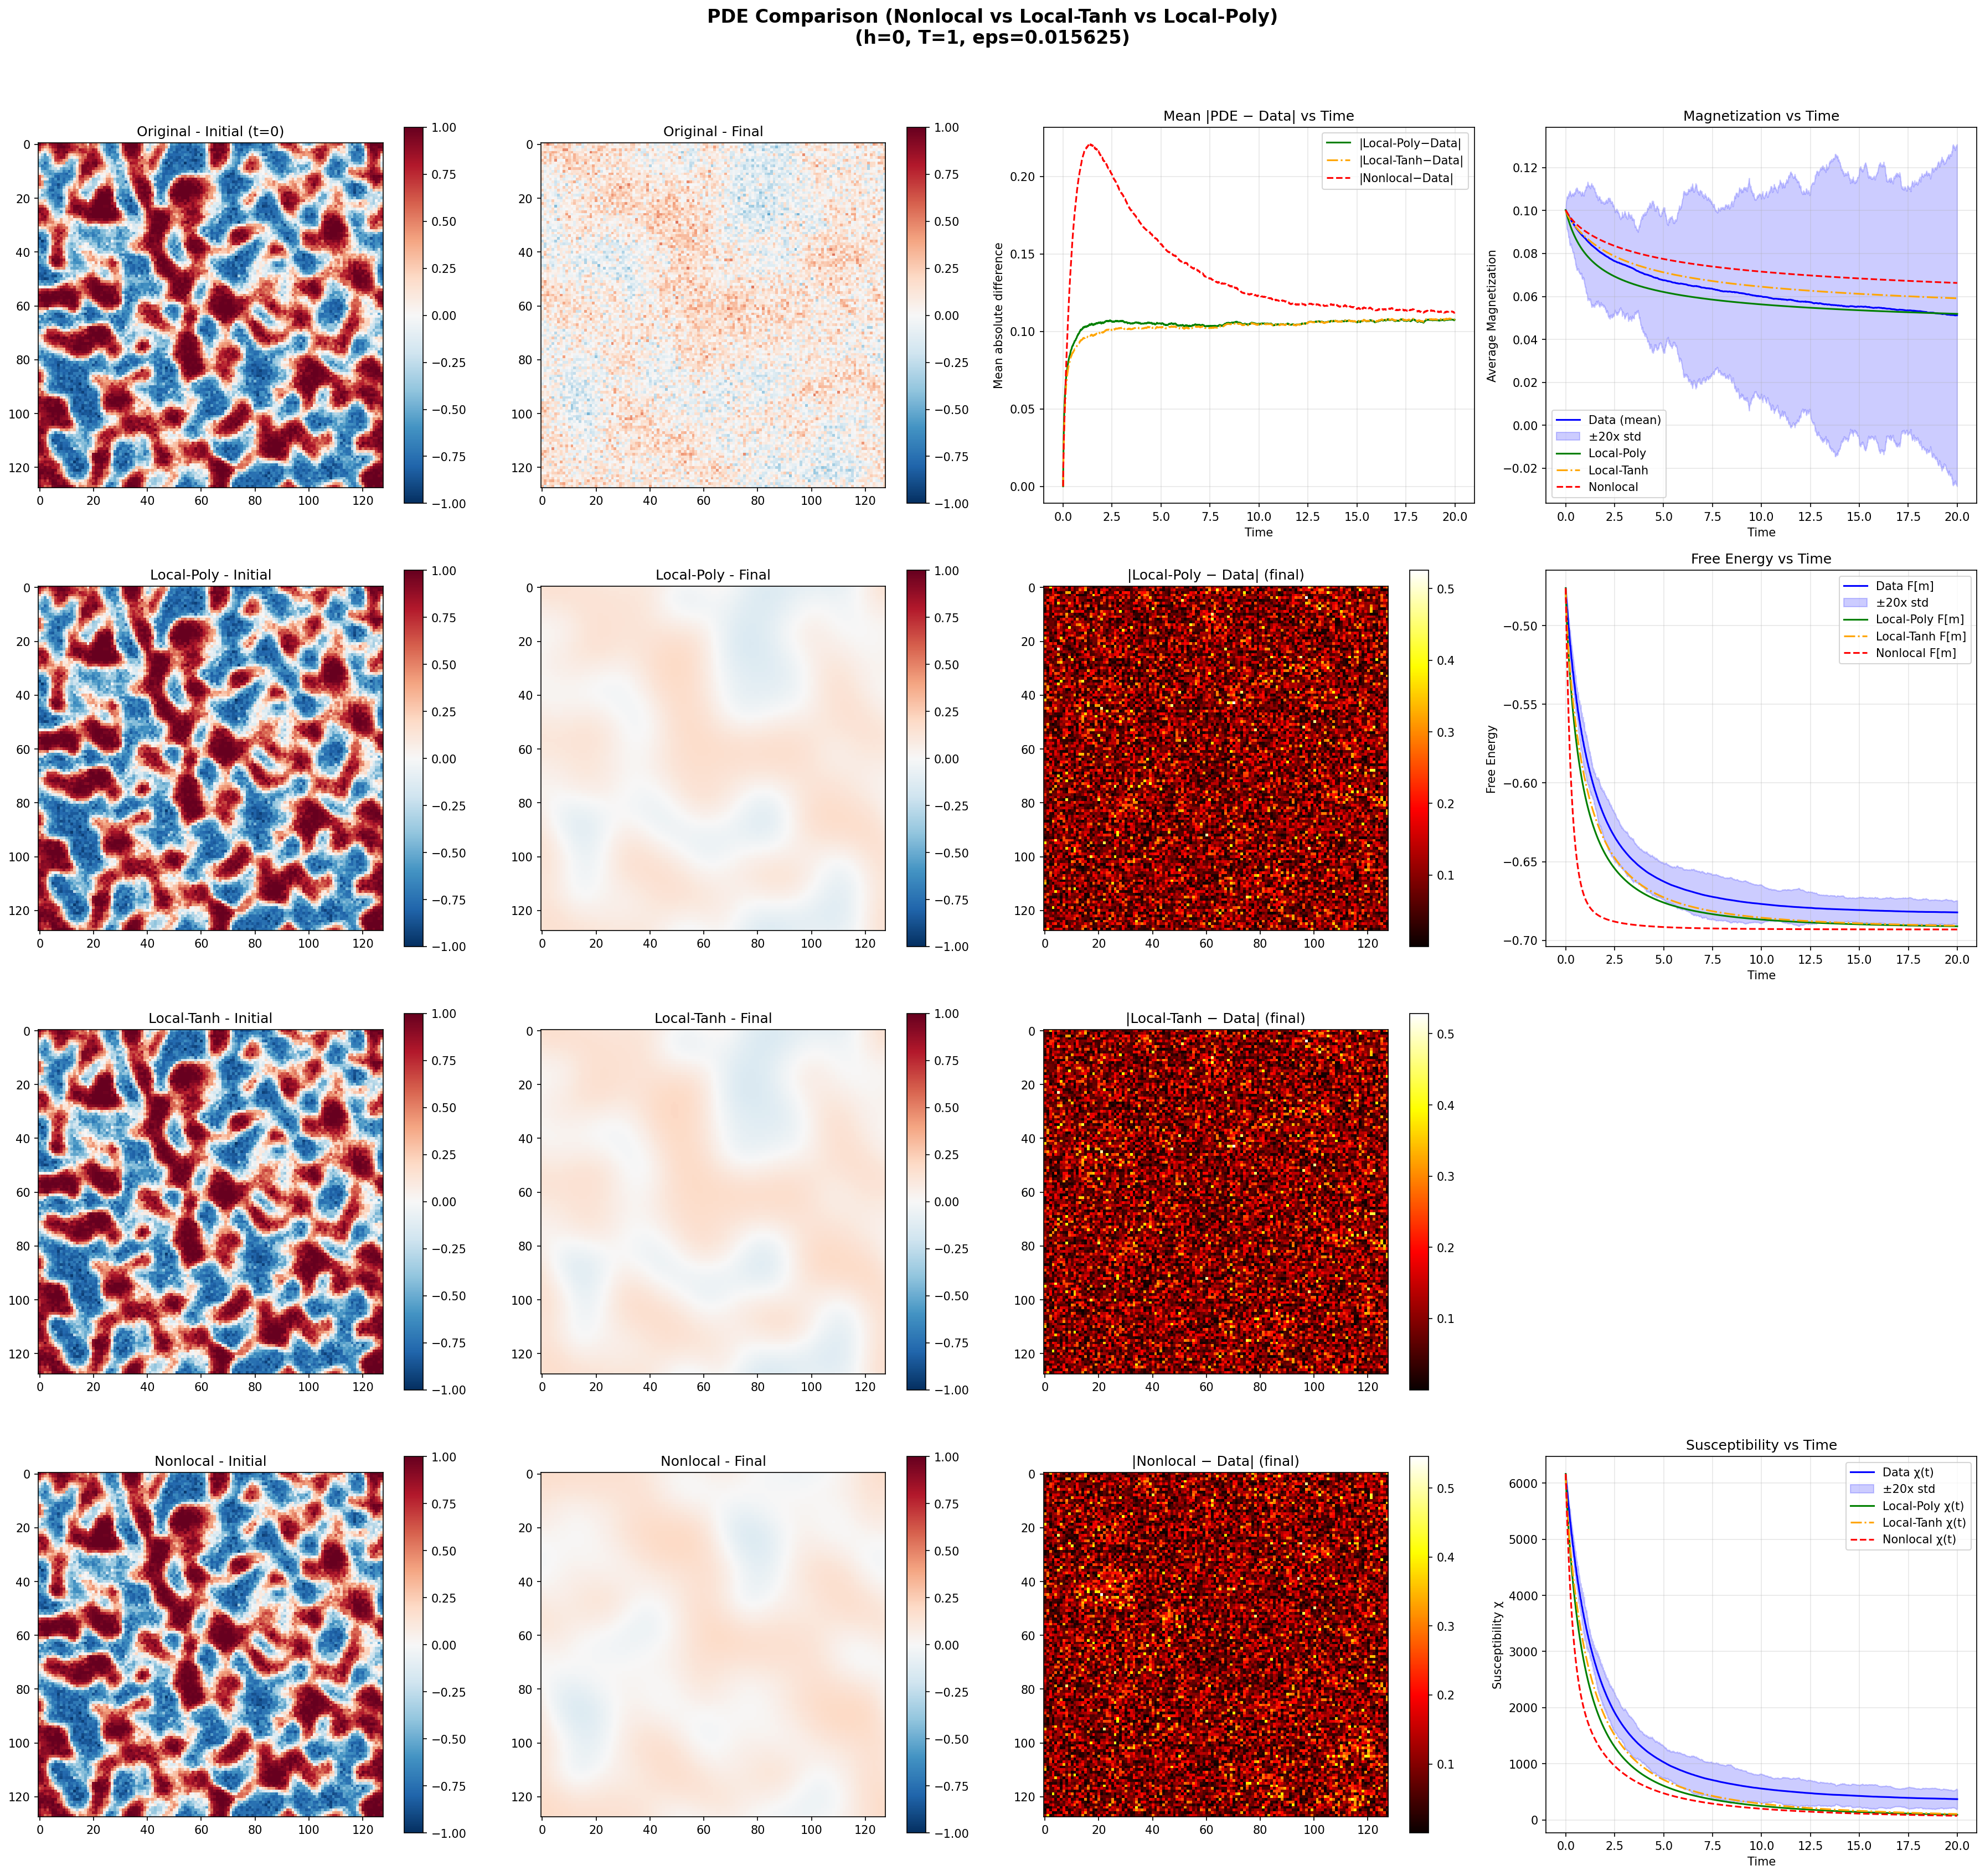
\includegraphics[width=1.0\textwidth]{fig/compare_pde_solvers_L1024_h0_T1_eps0.015625.png}
% 	\caption{Comparison of original data and PDE solutions for $h=0$, $T=1$, $\epsilon=0.015625$, $L=1024$.}
% 	\label{fig:pde_comparison_h0_T1_eps0.015625}
% \end{figure}


% \begin{figure}[!h]
% 	\centering
% 	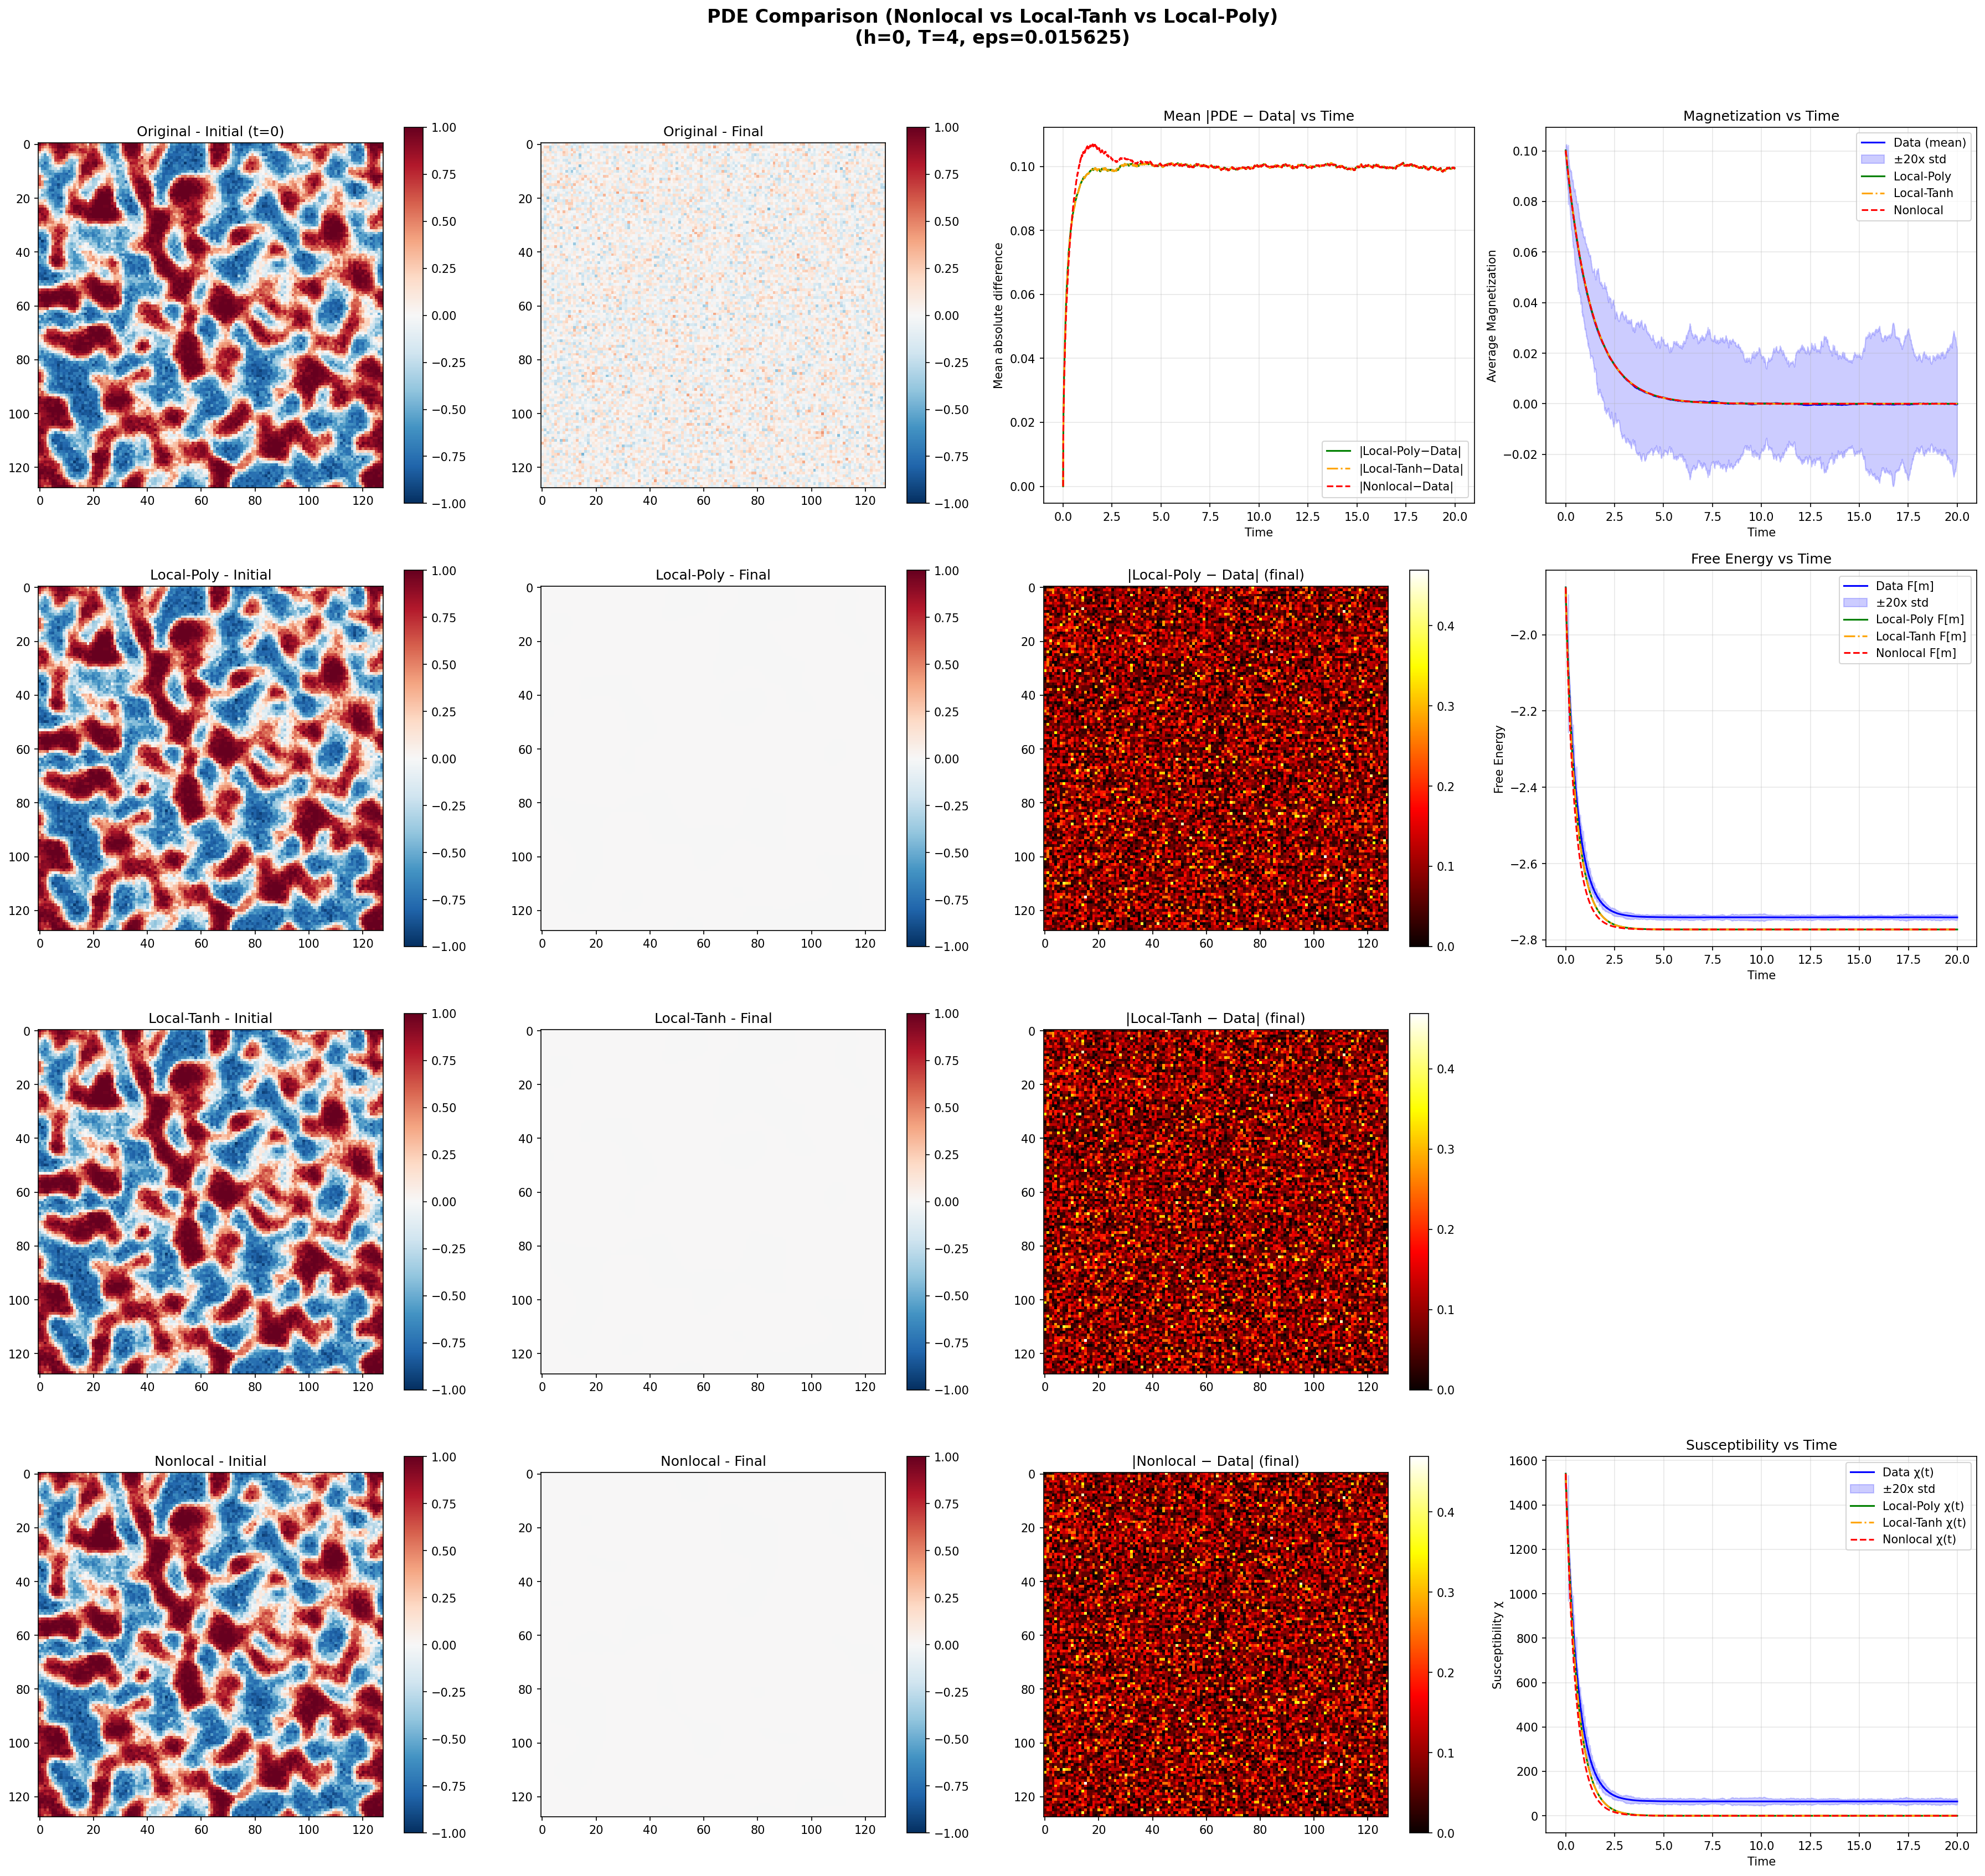
\includegraphics[width=1.0\textwidth]{fig/compare_pde_solvers_L1024_h0_T4_eps0.015625.png}
% 	\caption{Comparison of original data and PDE solutions for $h=0$, $T=4$, $\epsilon=0.015625$, $L=1024$.}
% 	\label{fig:pde_comparison_h0_T4_eps0.015625}
% \end{figure}


% \begin{figure}[!h]
% 	\centering
% 	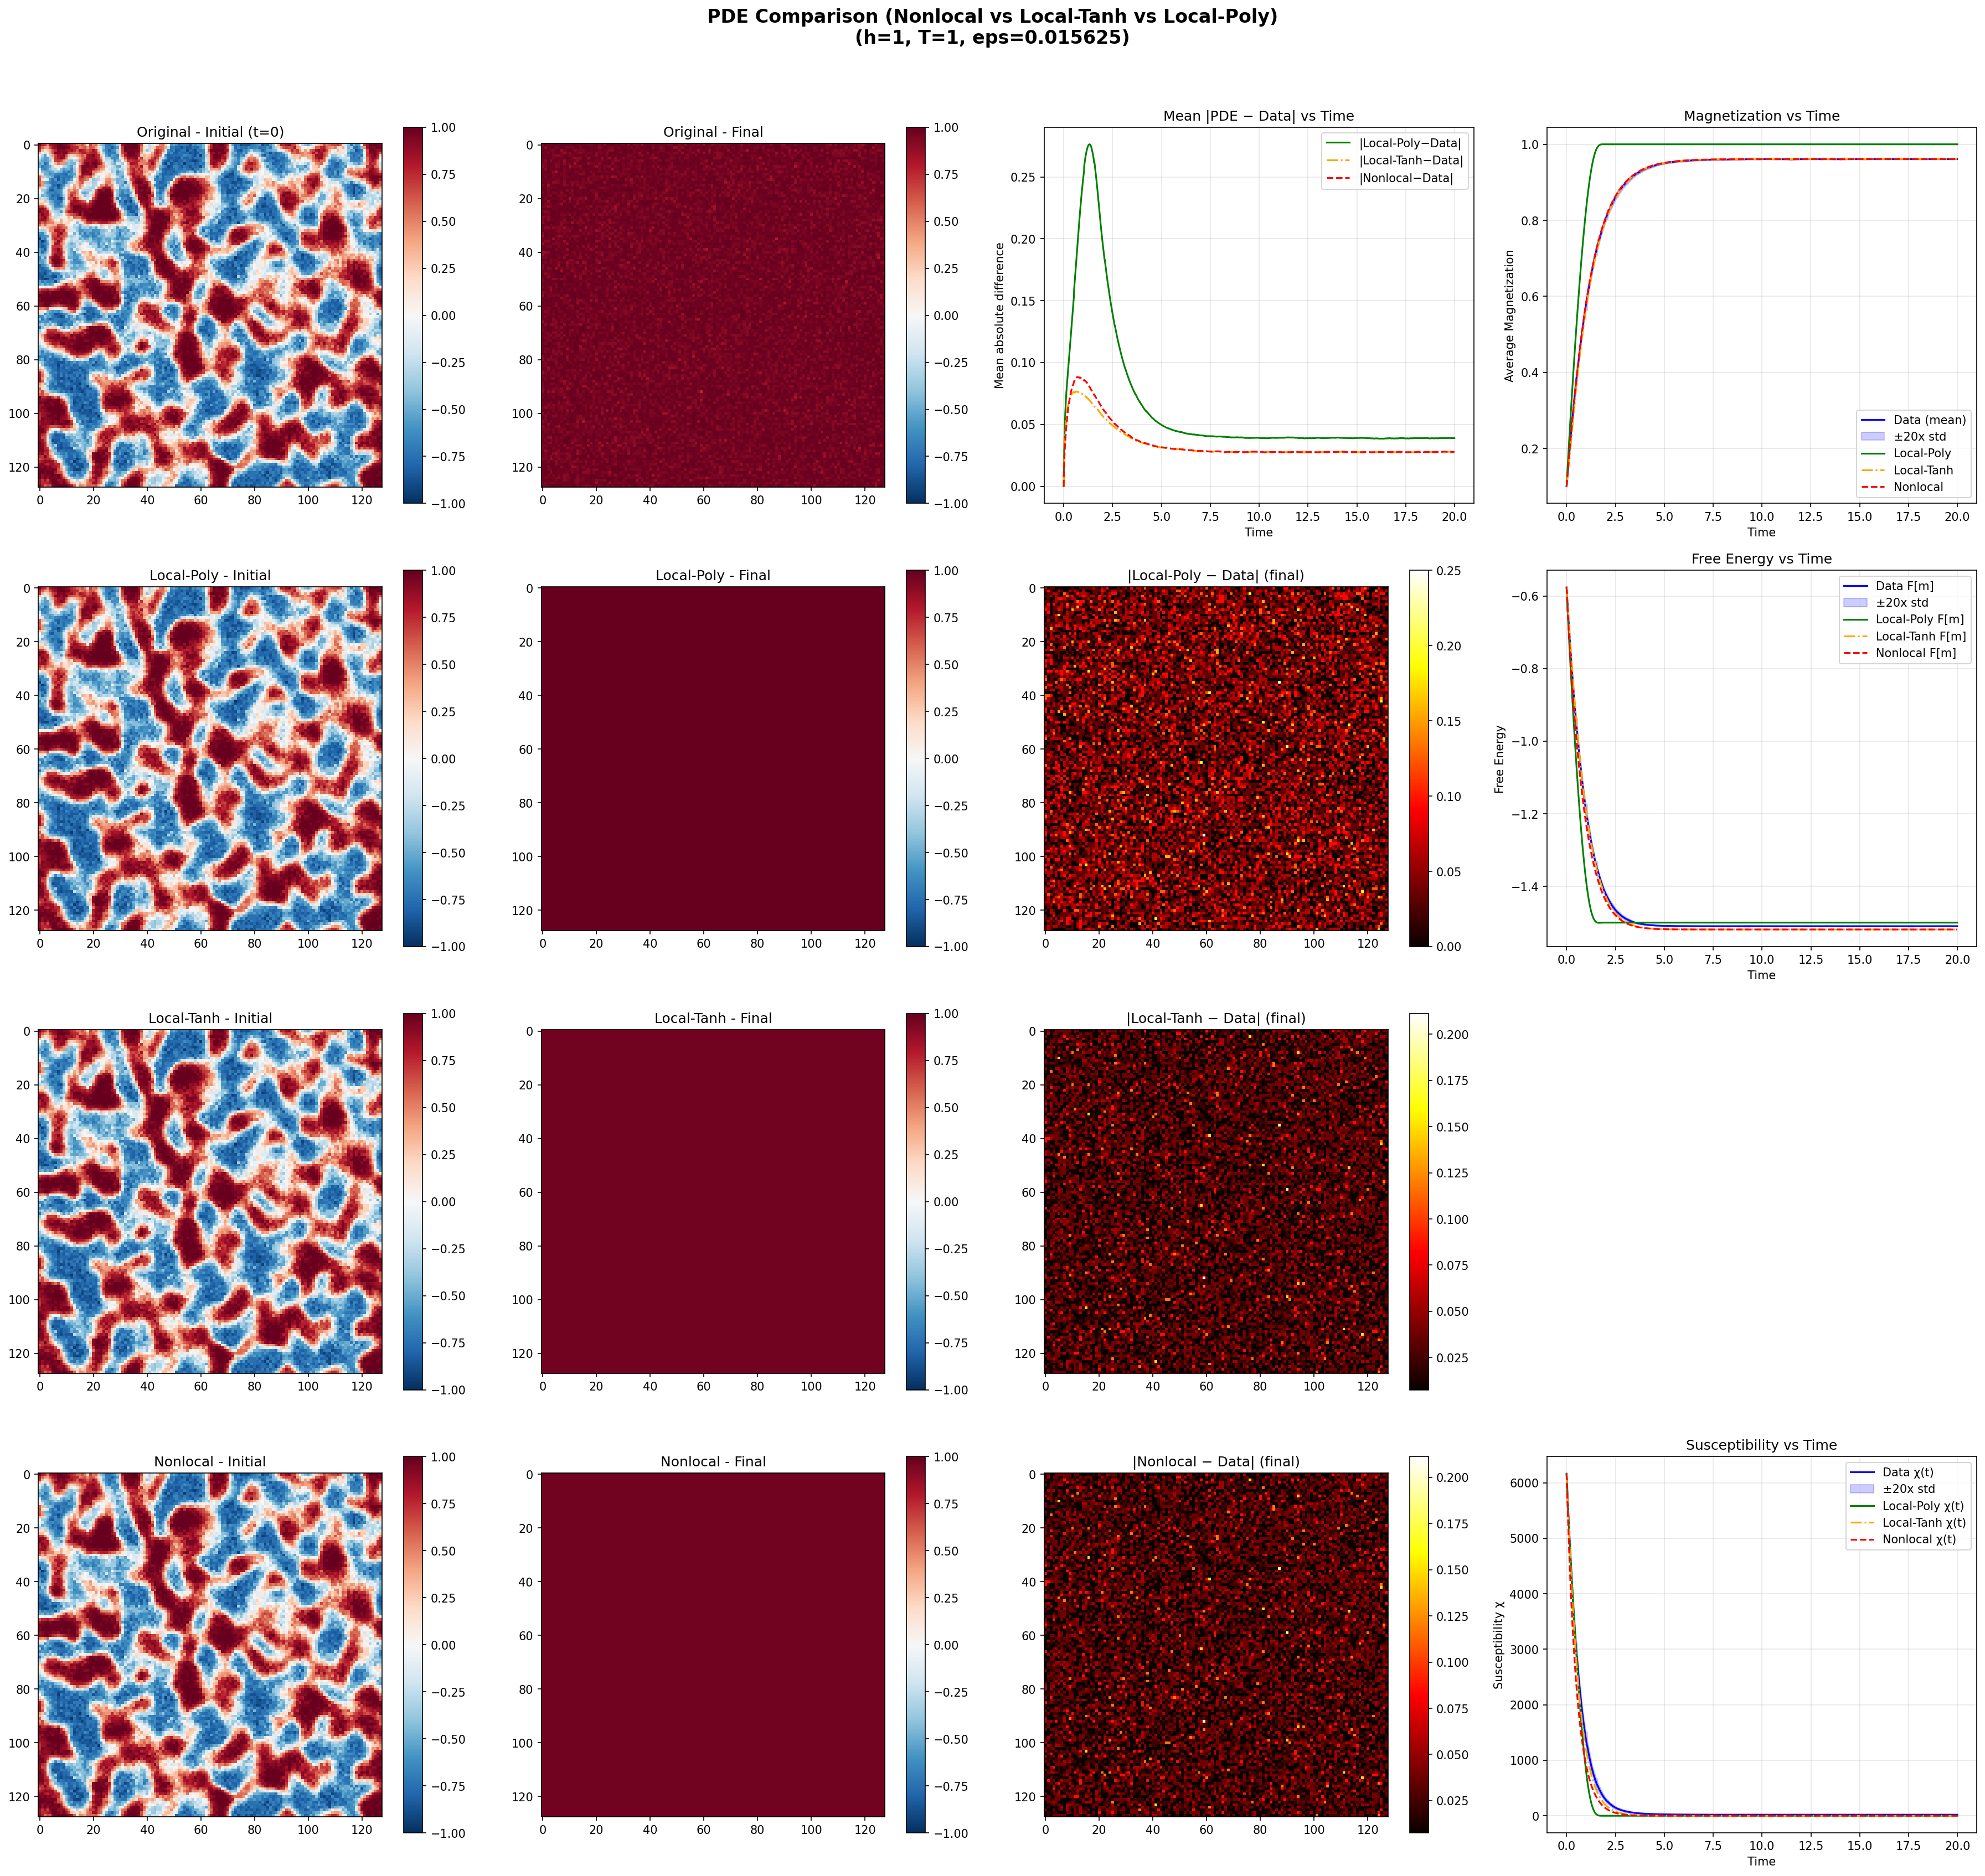
\includegraphics[width=1.0\textwidth]{fig/compare_pde_solvers_L1024_h1_T1_eps0.015625.png}
% 	\caption{Comparison of original data and PDE solutions for $h=1$, $T=1$, $\epsilon=0.015625$, $L=1024$.}
% 	\label{fig:pde_comparison_h1_T1_eps0.015625}
% \end{figure}


% \begin{figure}[!h]
% 	\centering
% 	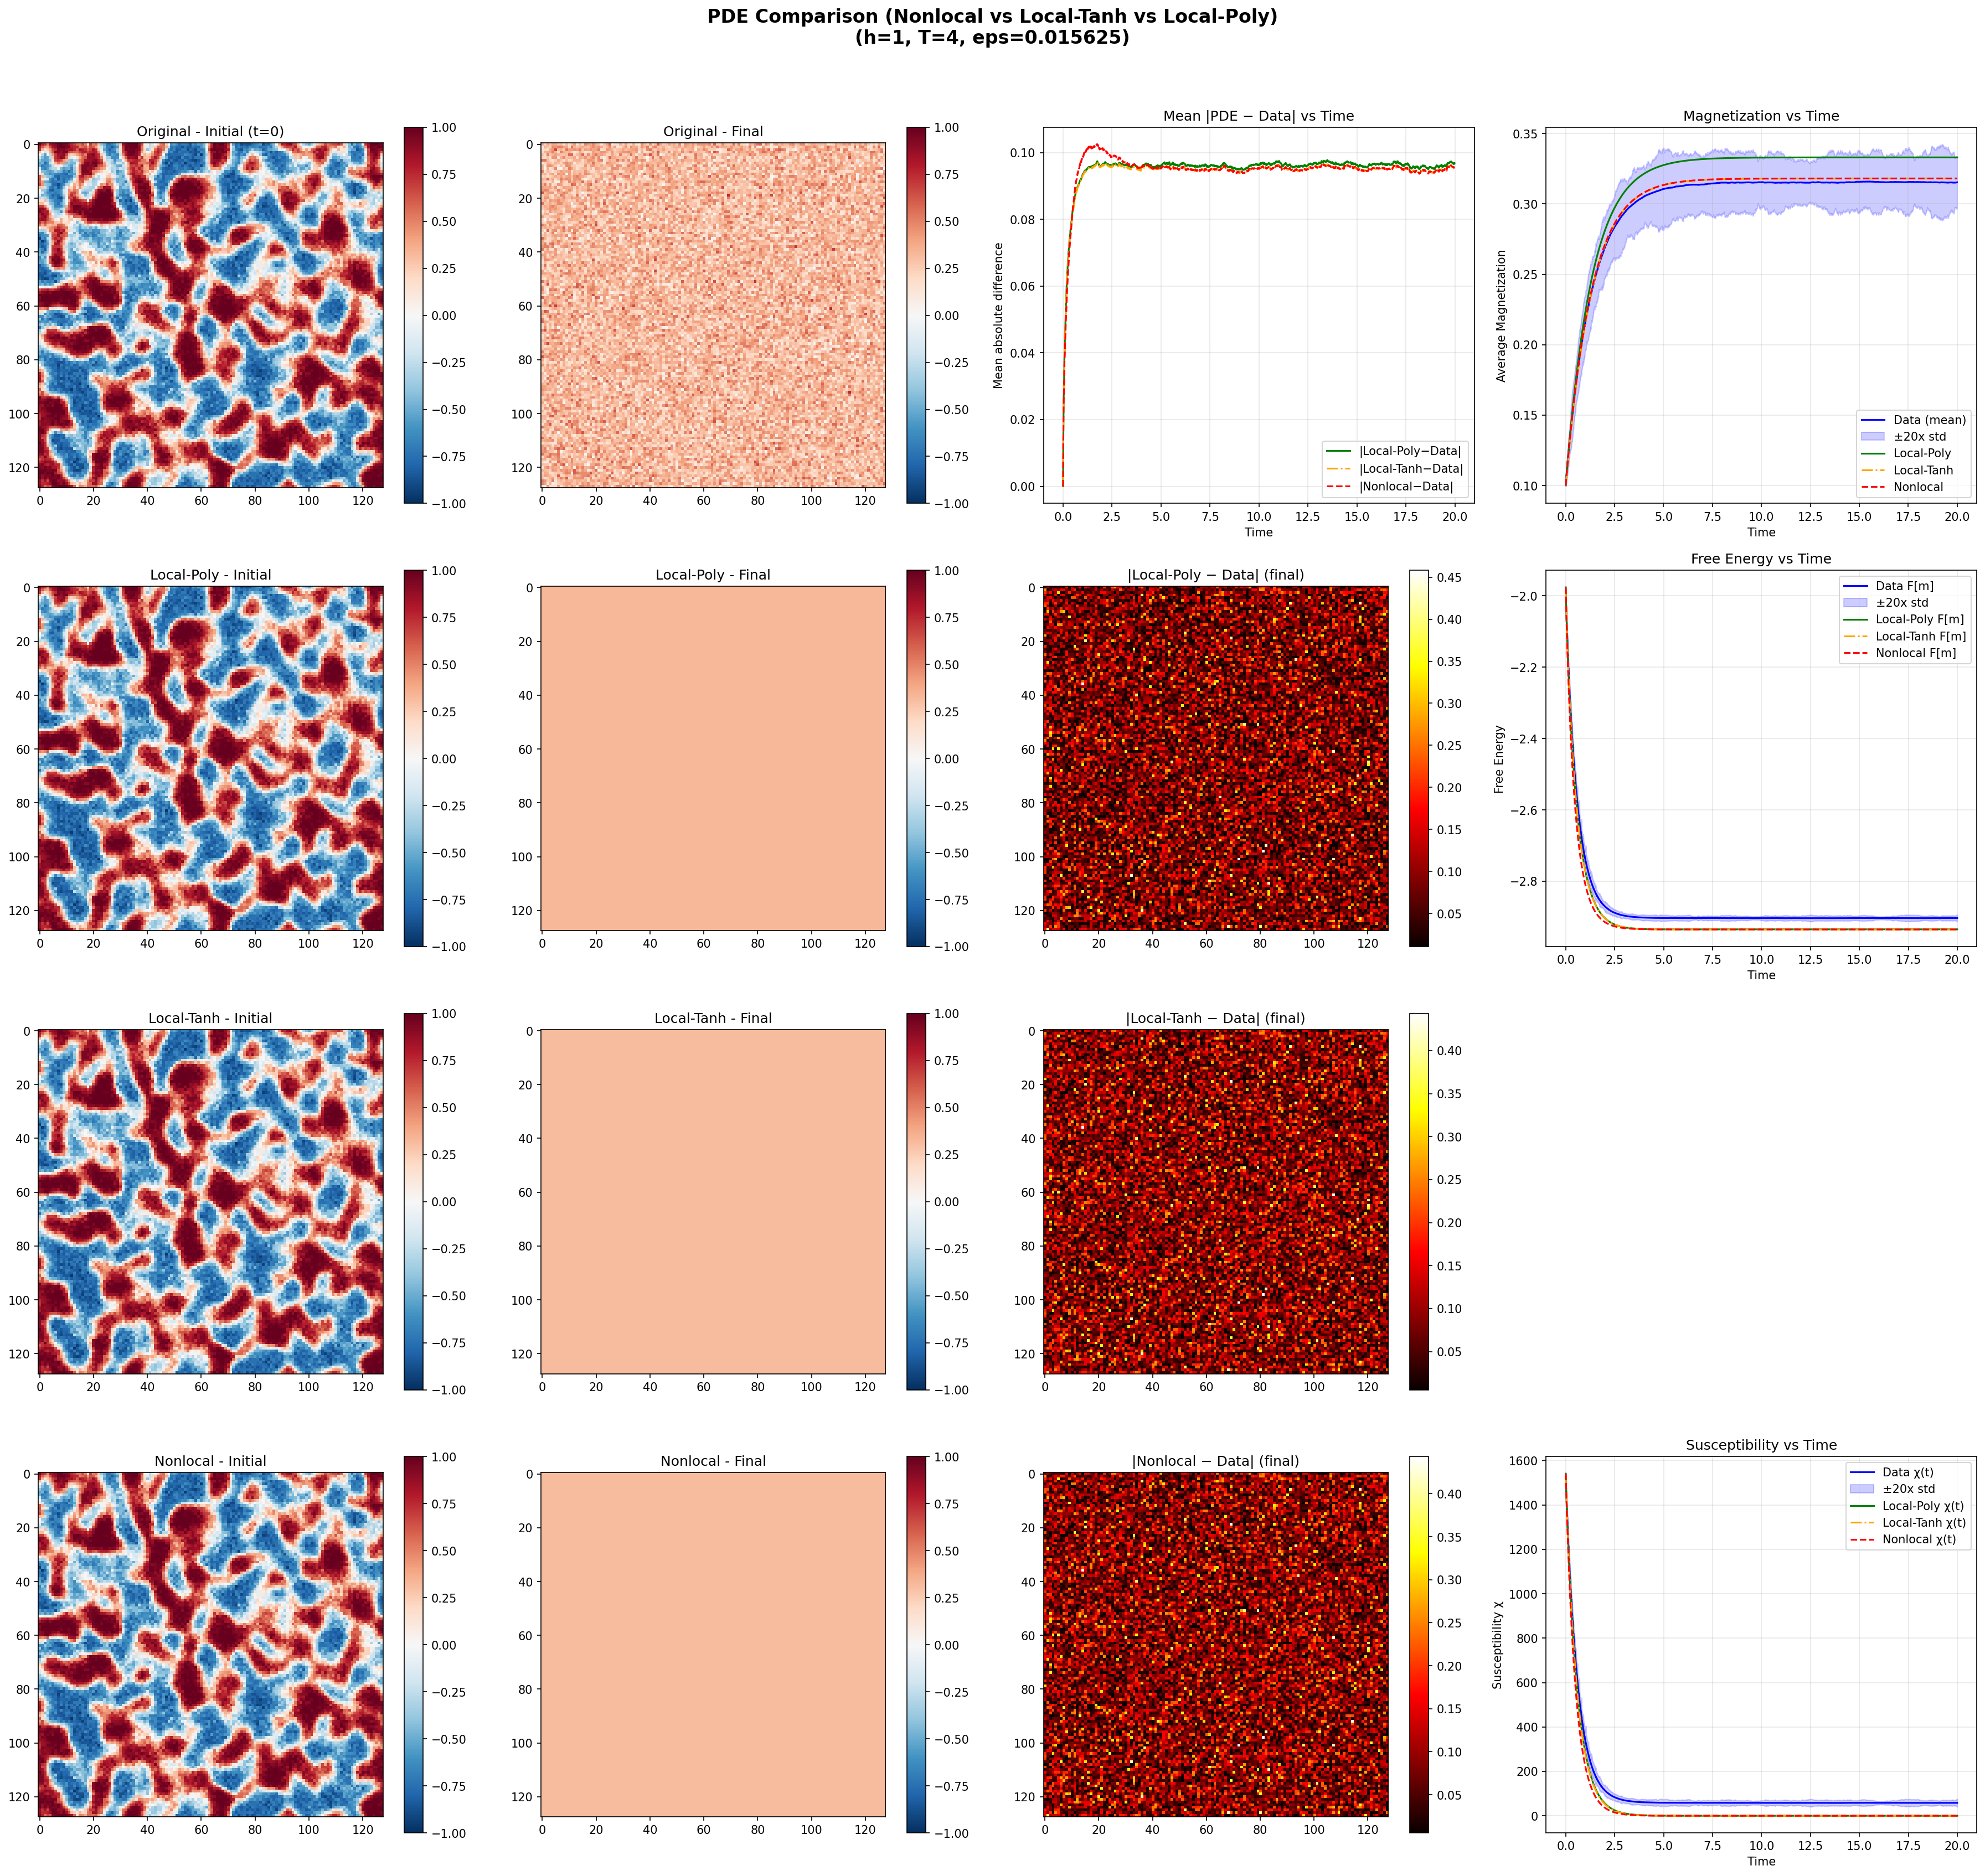
\includegraphics[width=1.0\textwidth]{fig/compare_pde_solvers_L1024_h1_T4_eps0.015625.png}
% 	\caption{Comparison of original data and PDE solutions for $h=1$, $T=4$, $\epsilon=0.015625$, $L=1024$.}
% 	\label{fig:pde_comparison_h1_T4_eps0.015625}
% \end{figure}

% % with epsilon = 0.03125

% \begin{figure}[!h]
% 	\centering
% 	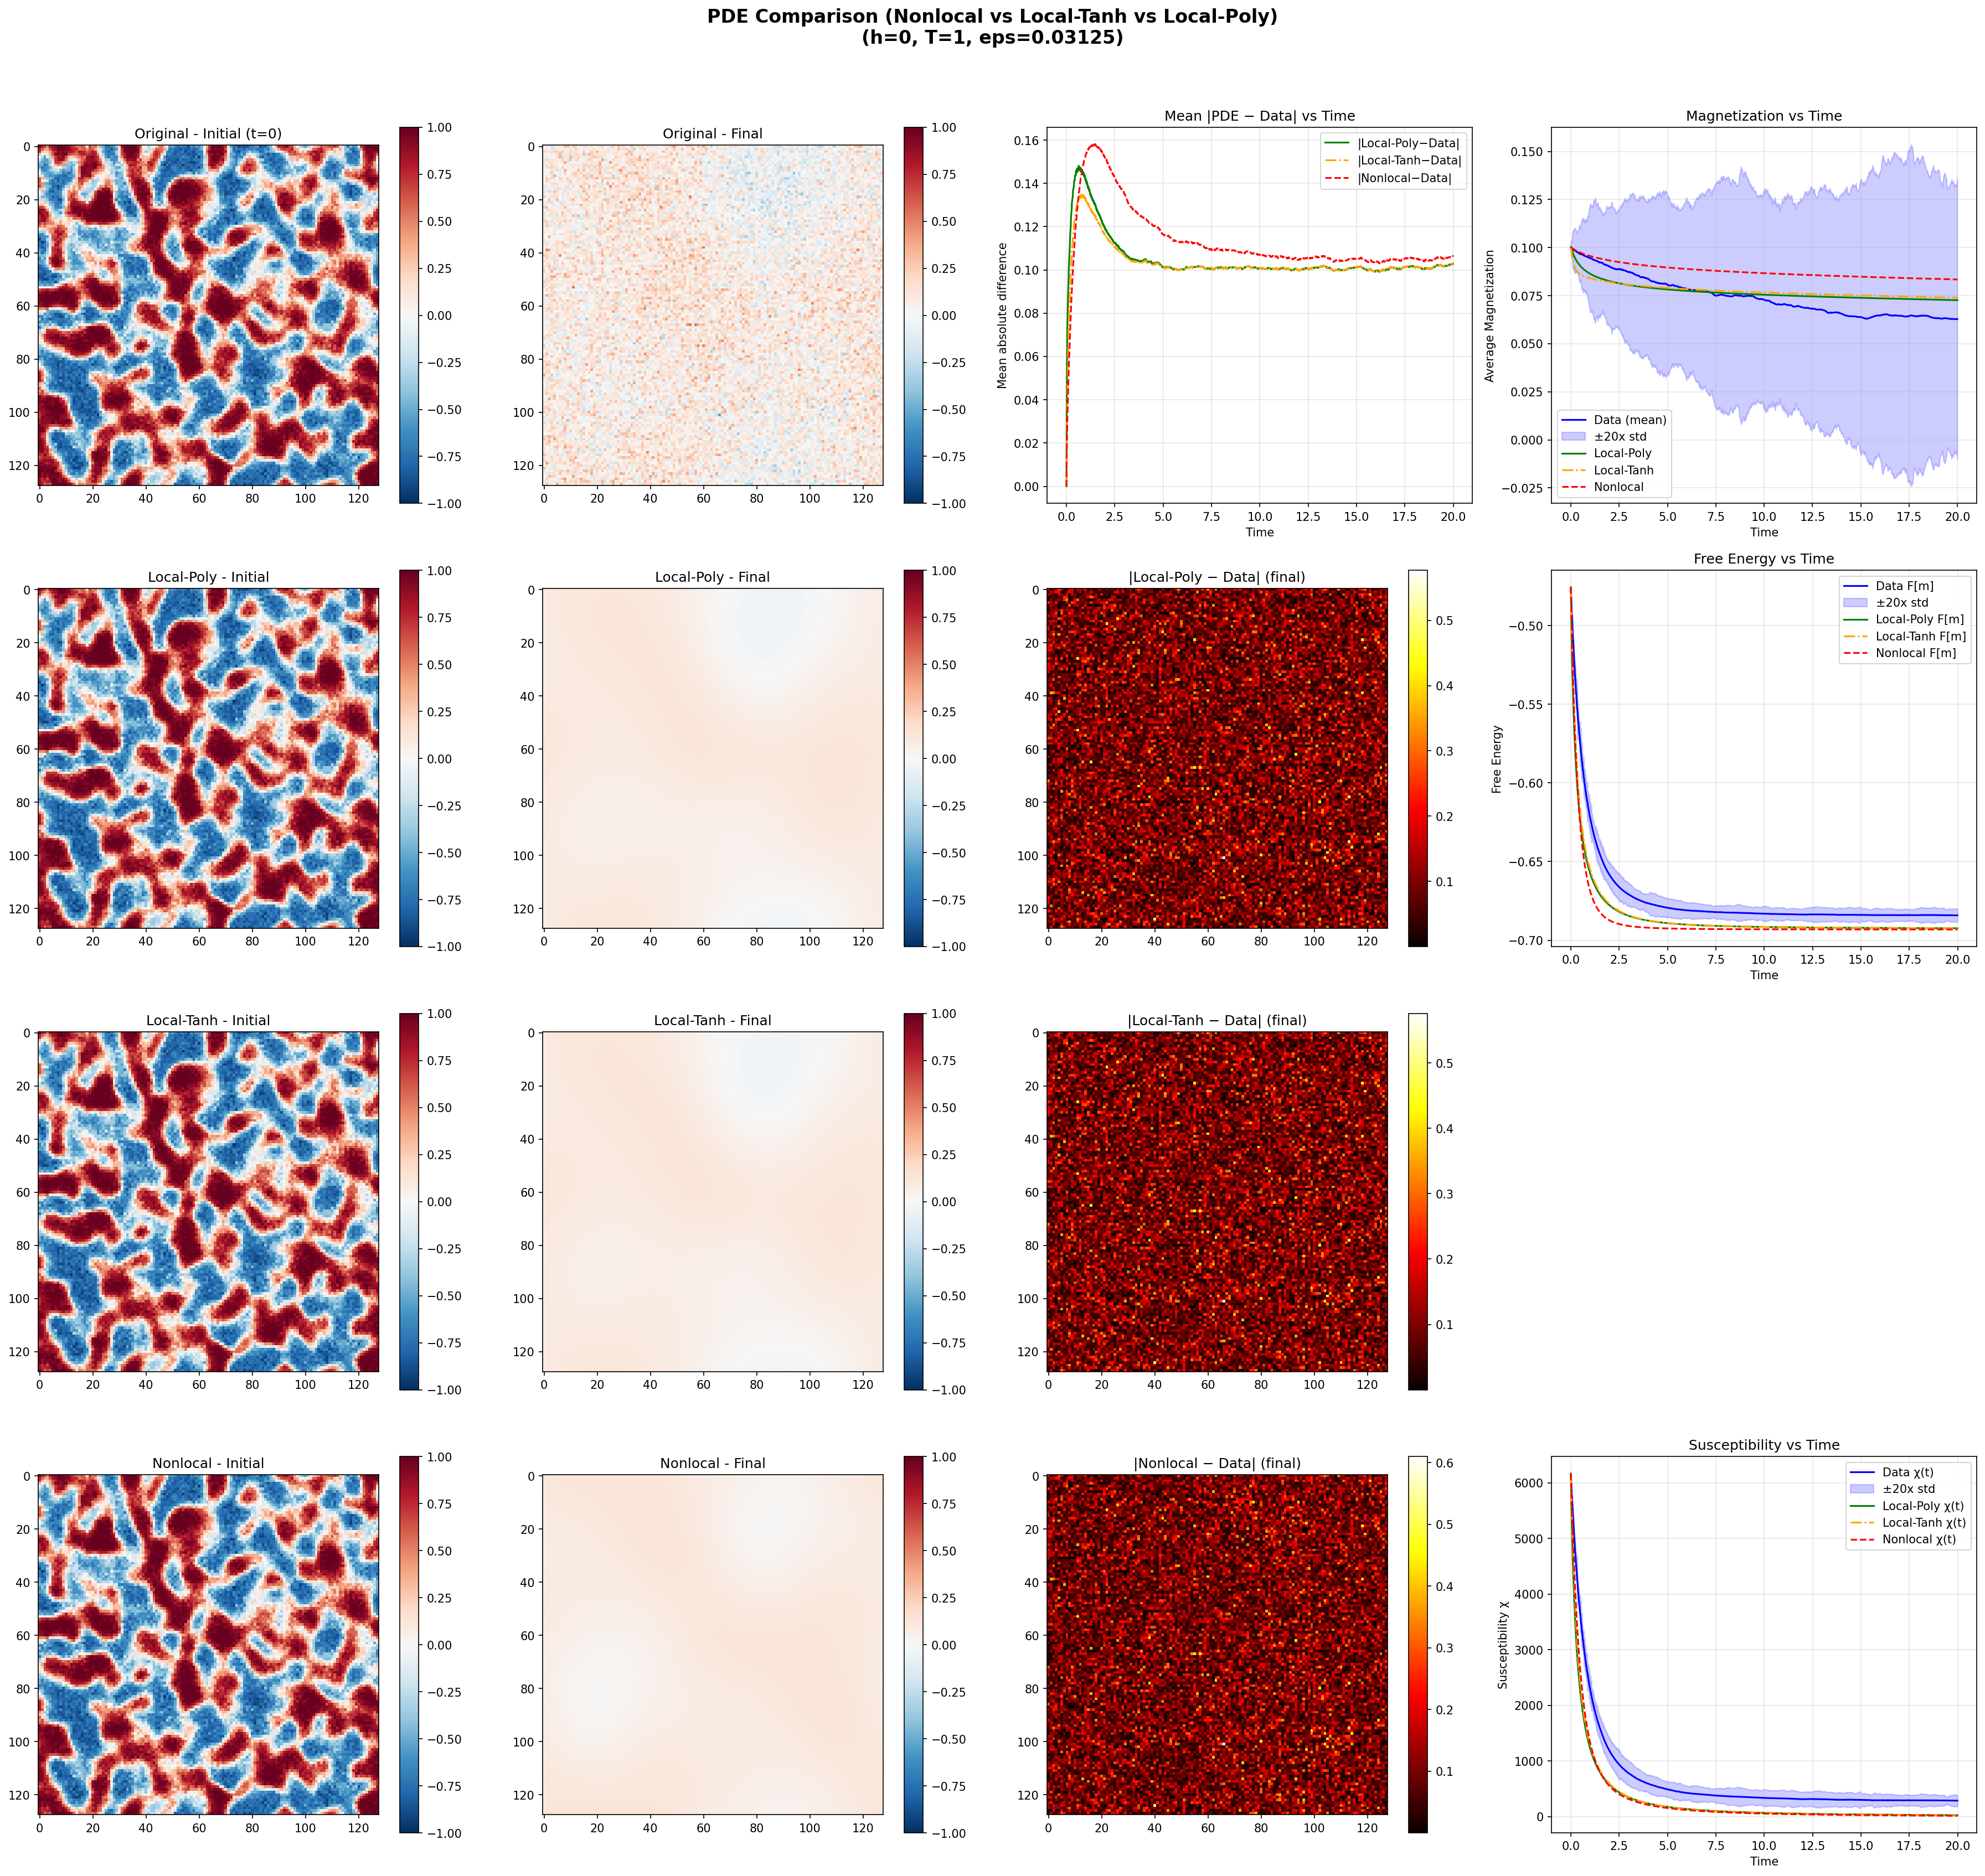
\includegraphics[width=1.0\textwidth]{fig/compare_pde_solvers_L1024_h0_T1_eps0.03125.png}
% 	\caption{Comparison of original data and PDE solutions for $h=0$, $T=1$, $\epsilon=0.03125$, $L=1024$.}
% 	\label{fig:pde_comparison_h0_T1_eps0.03125}
% \end{figure}


% \begin{figure}[h]
% 	\centering
% 	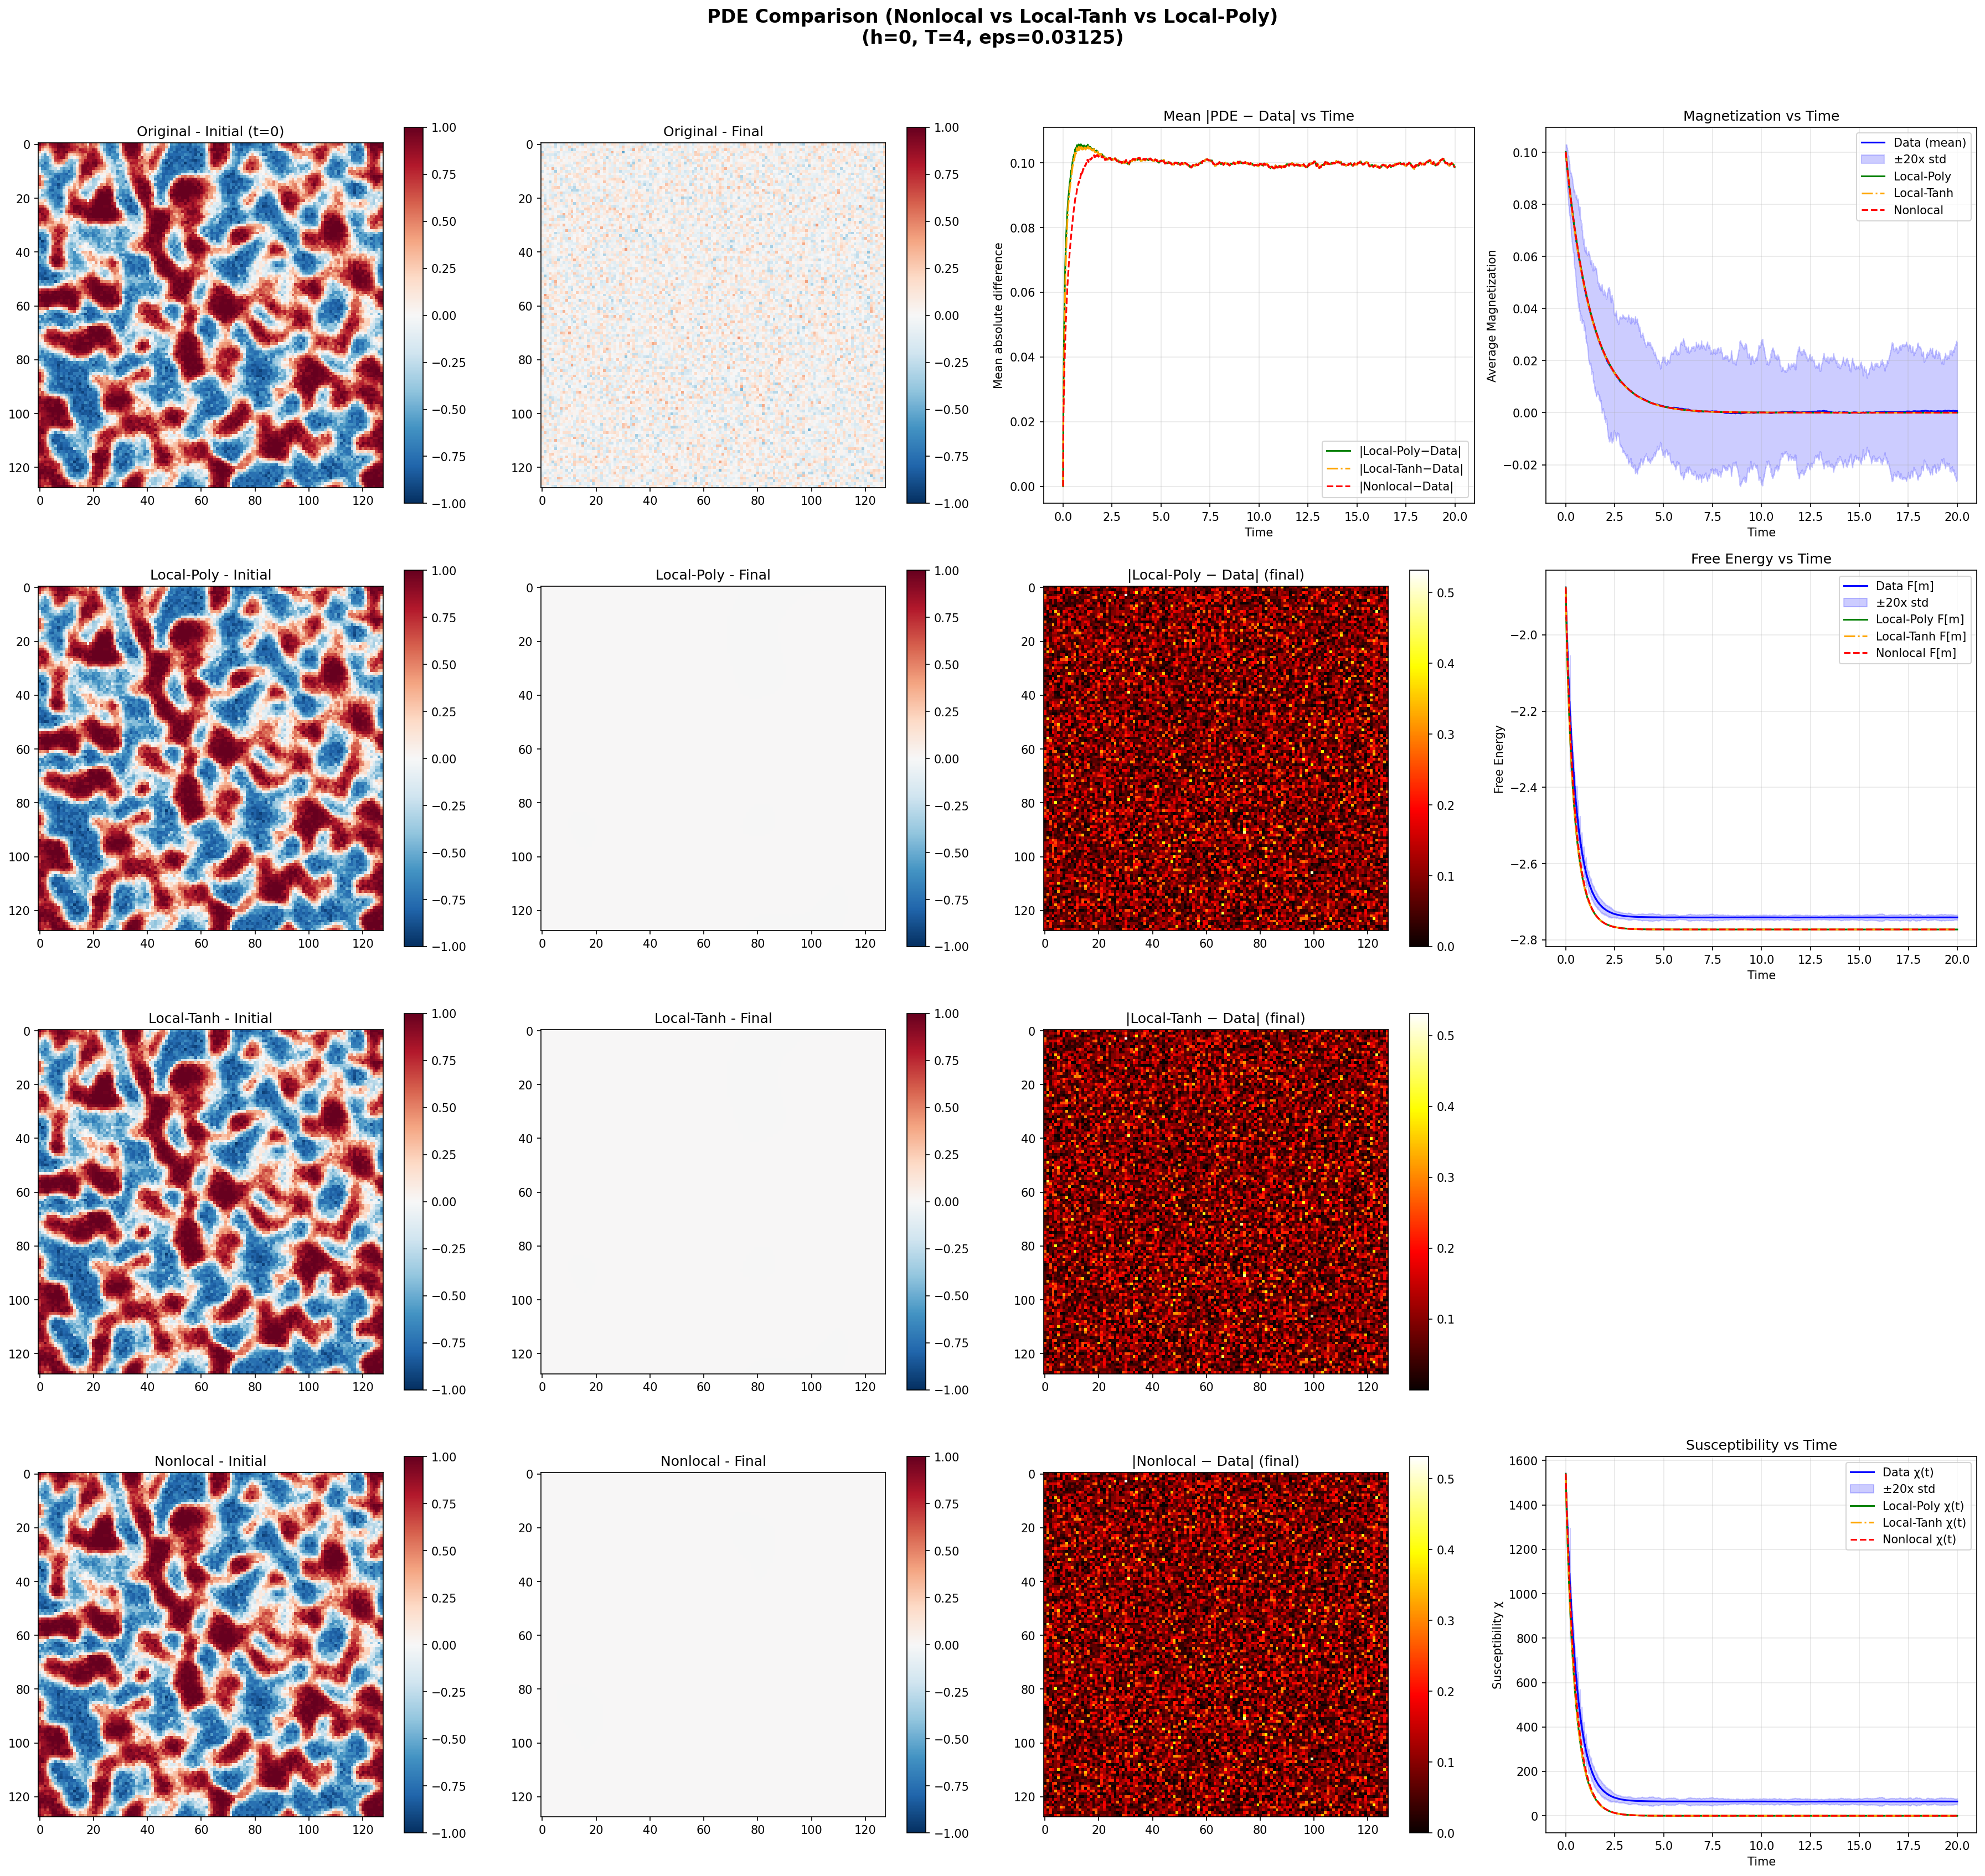
\includegraphics[width=1.0\textwidth]{fig/compare_pde_solvers_L1024_h0_T4_eps0.03125.png}
% 	\caption{Comparison of original data and PDE solutions for $h=0$, $T=4$, $\epsilon=0.03125$, $L=1024$.}
% 	\label{fig:pde_comparison_h0_T4_eps0.03125}
% \end{figure}


% \begin{figure}[!h]
% 	\centering
% 	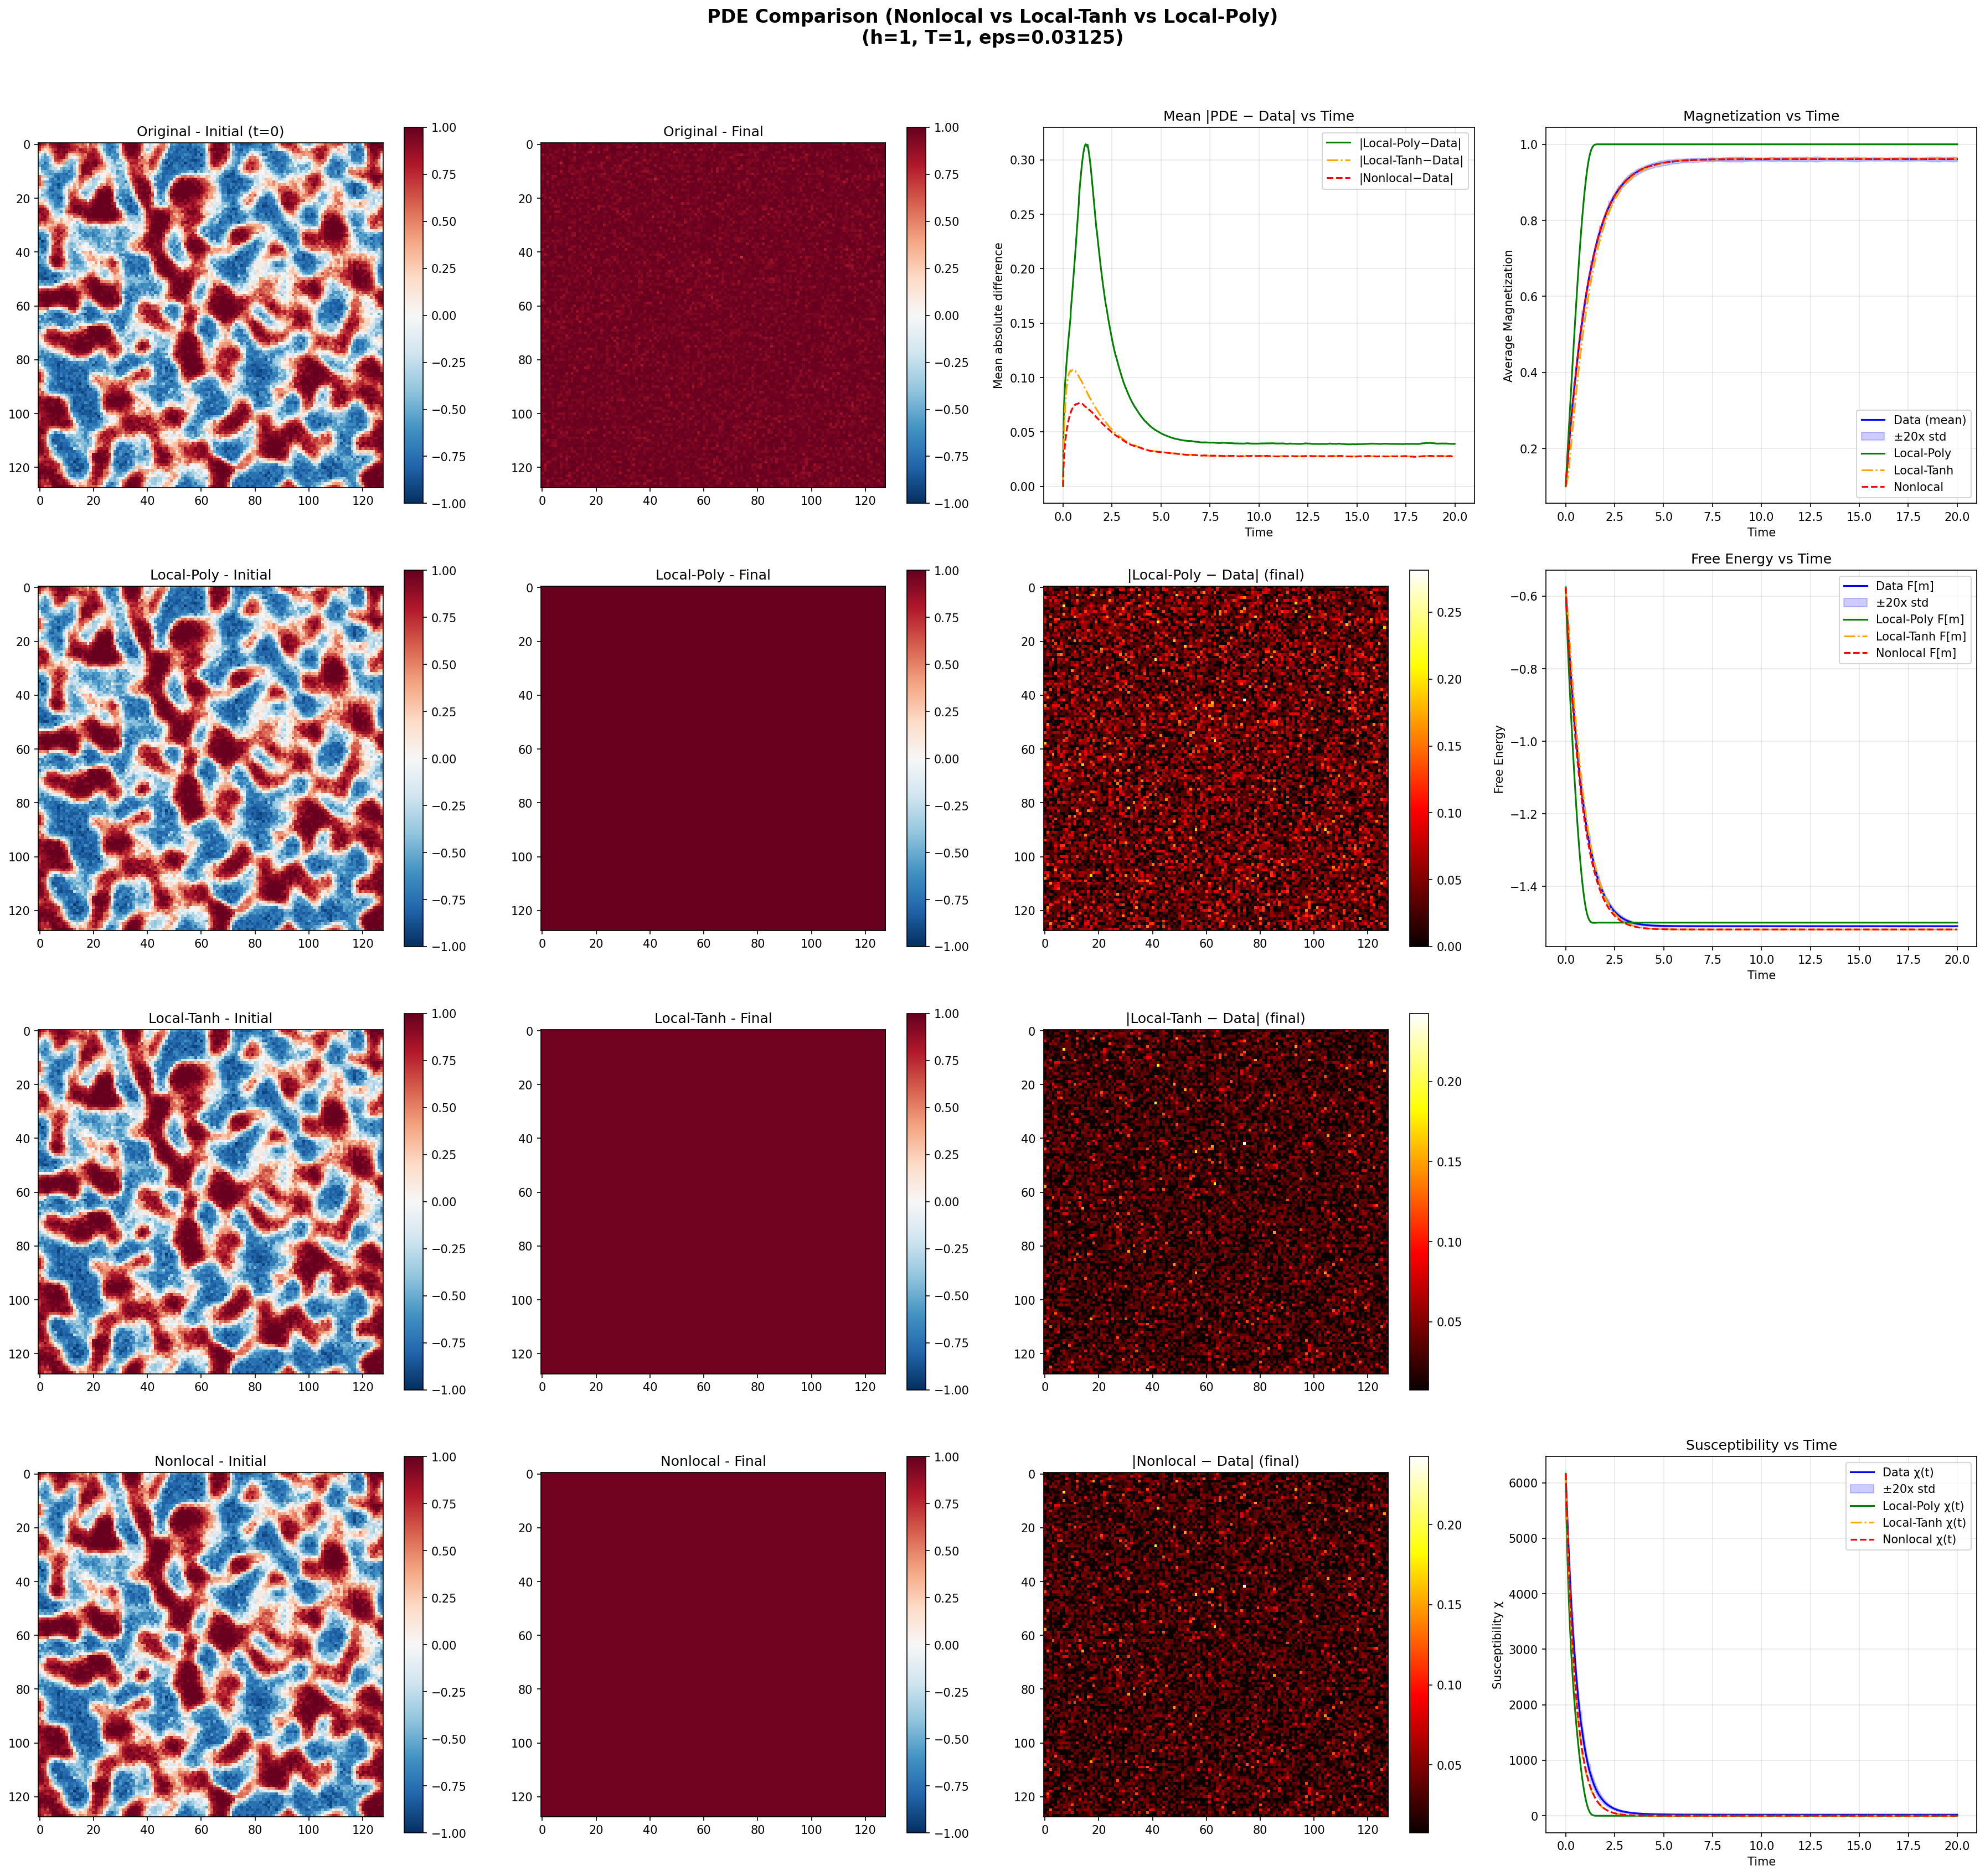
\includegraphics[width=1.0\textwidth]{fig/compare_pde_solvers_L1024_h1_T1_eps0.03125.png}
% 	\caption{Comparison of original data and PDE solutions for $h=1$, $T=1$, $\epsilon=0.03125$, $L=1024$.}
% 	\label{fig:pde_comparison_h1_T1_eps0.03125}
% \end{figure}


% \begin{figure}[h]
% 	\centering
% 	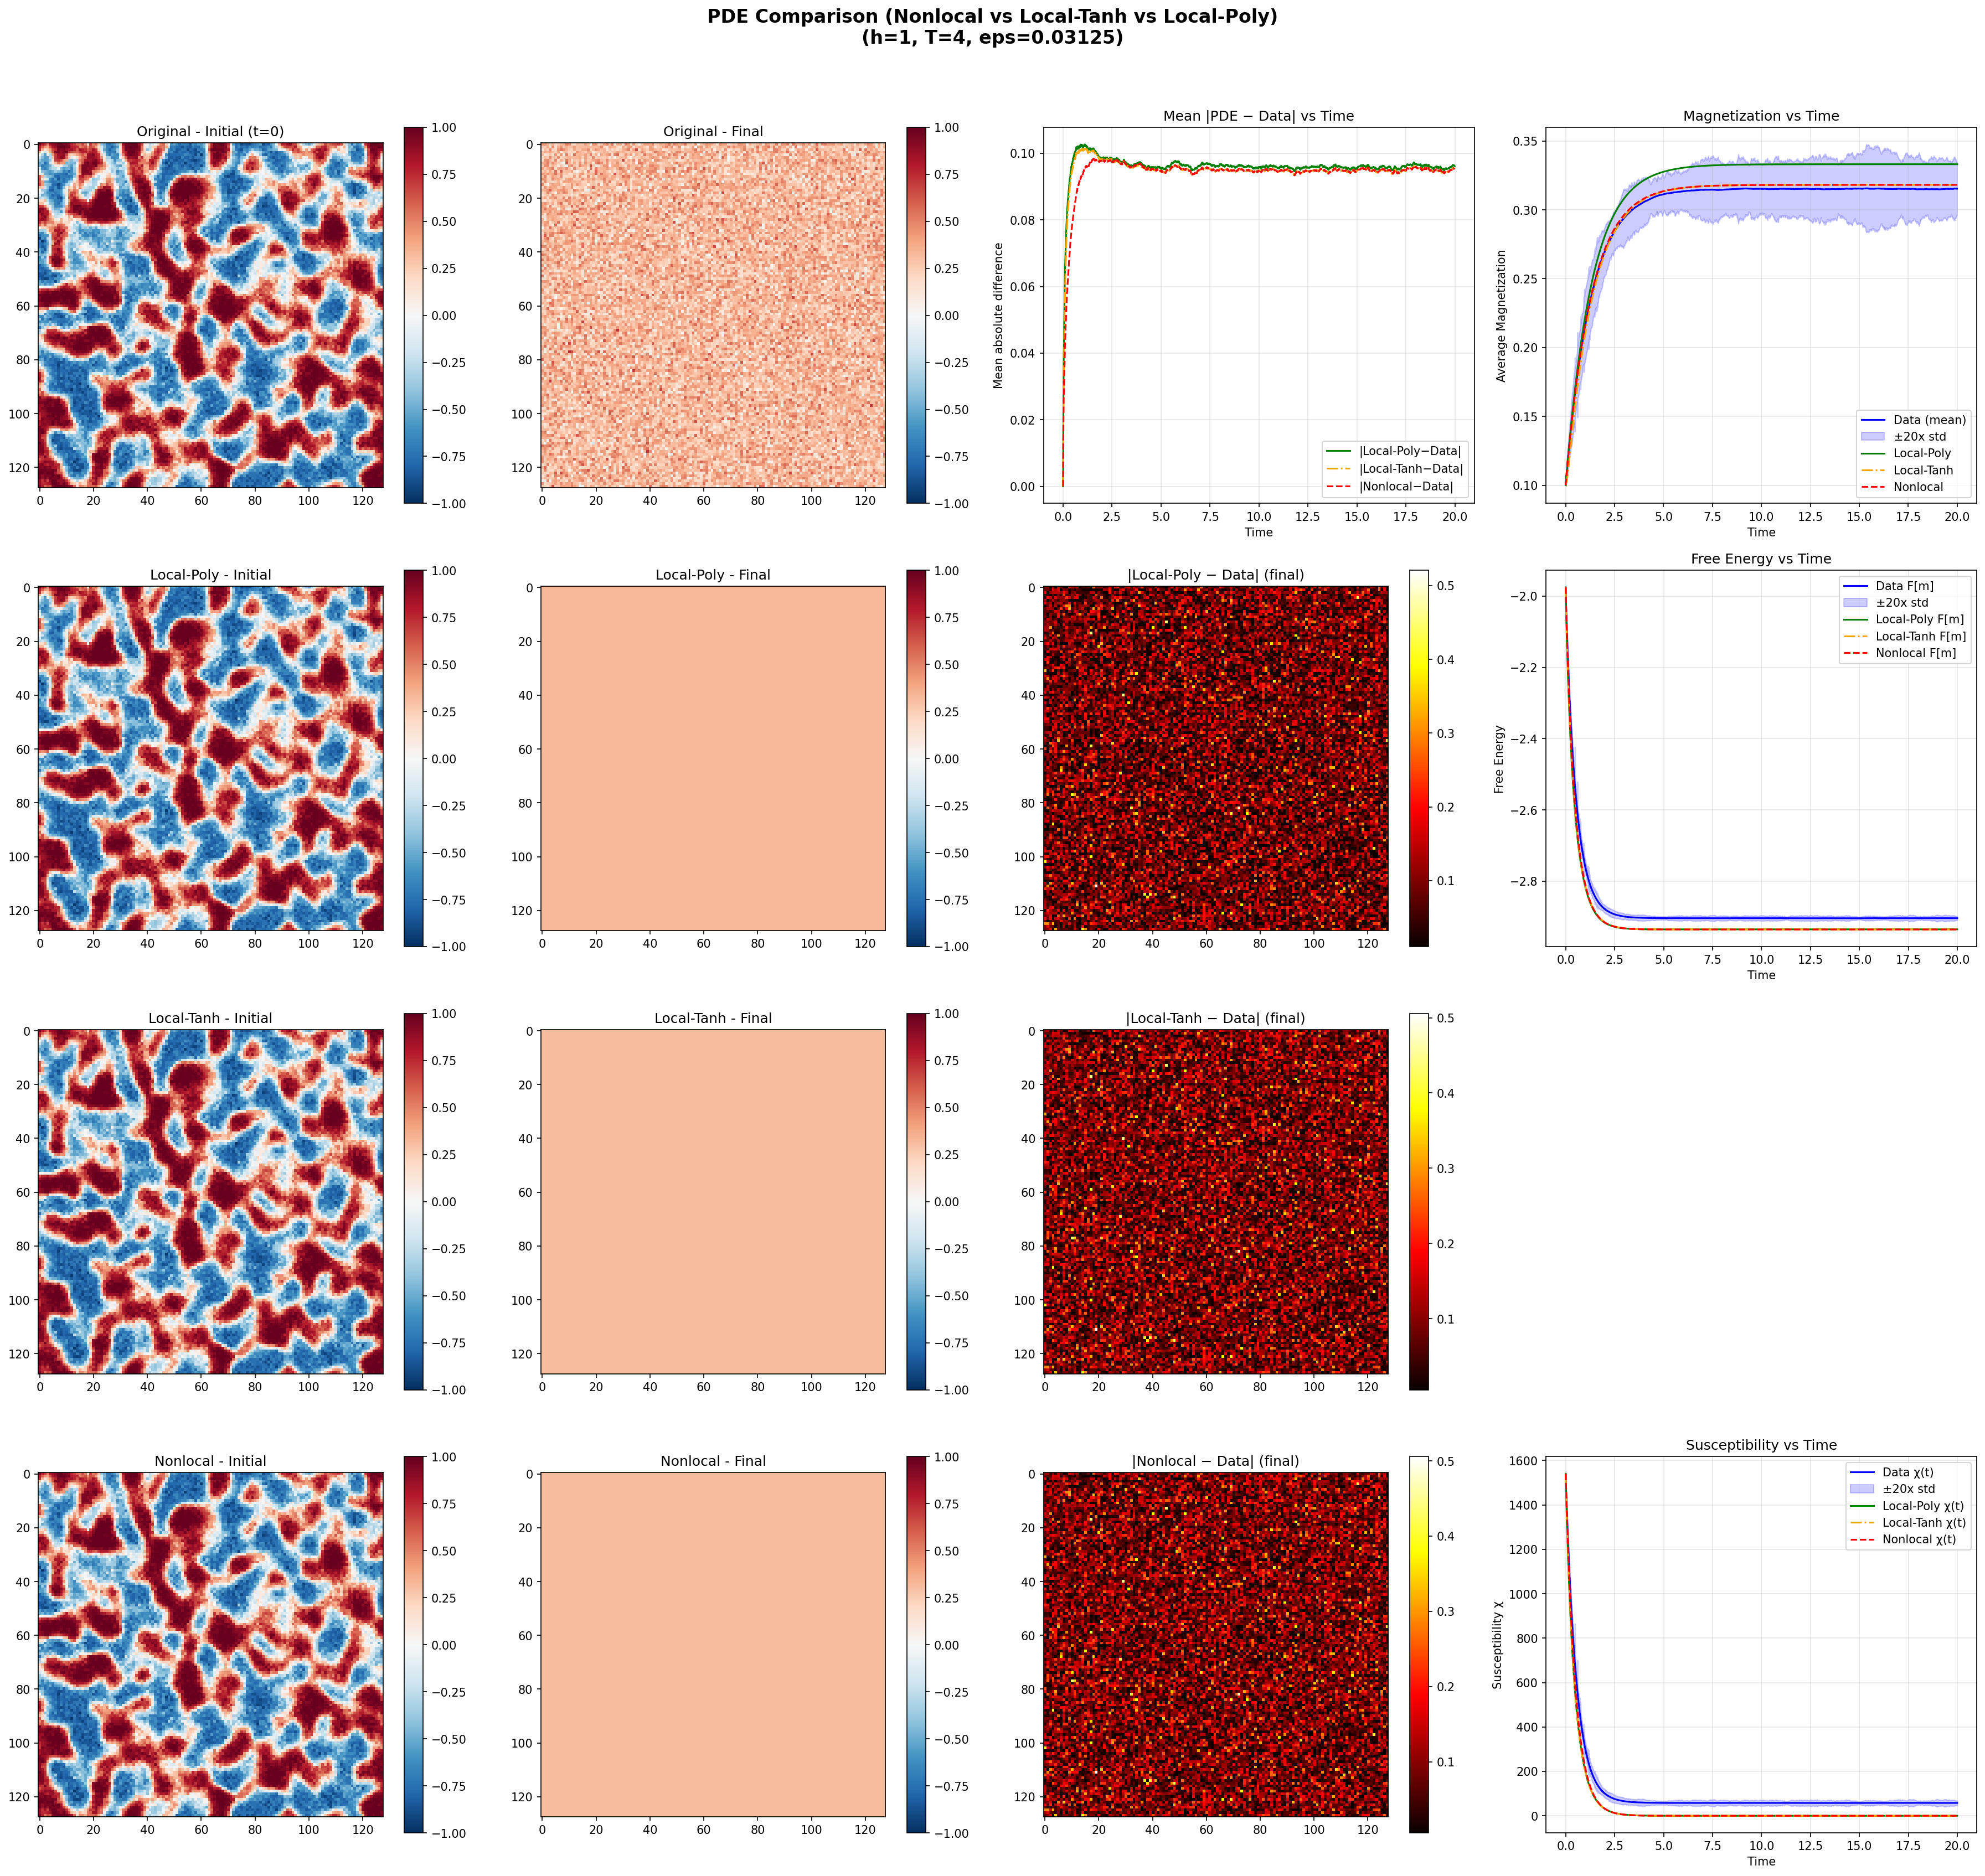
\includegraphics[width=1.0\textwidth]{fig/compare_pde_solvers_L1024_h1_T4_eps0.03125.png}
% 	\caption{Comparison of original data and PDE solutions for $h=1$, $T=4$, $\epsilon=0.03125$, $L=1024$.}
% 	\label{fig:pde_comparison_h1_T4_eps0.03125}
% \end{figure}


% % with epsilon = 0.0625

% \begin{figure}[!h]
% 	\centering
% 	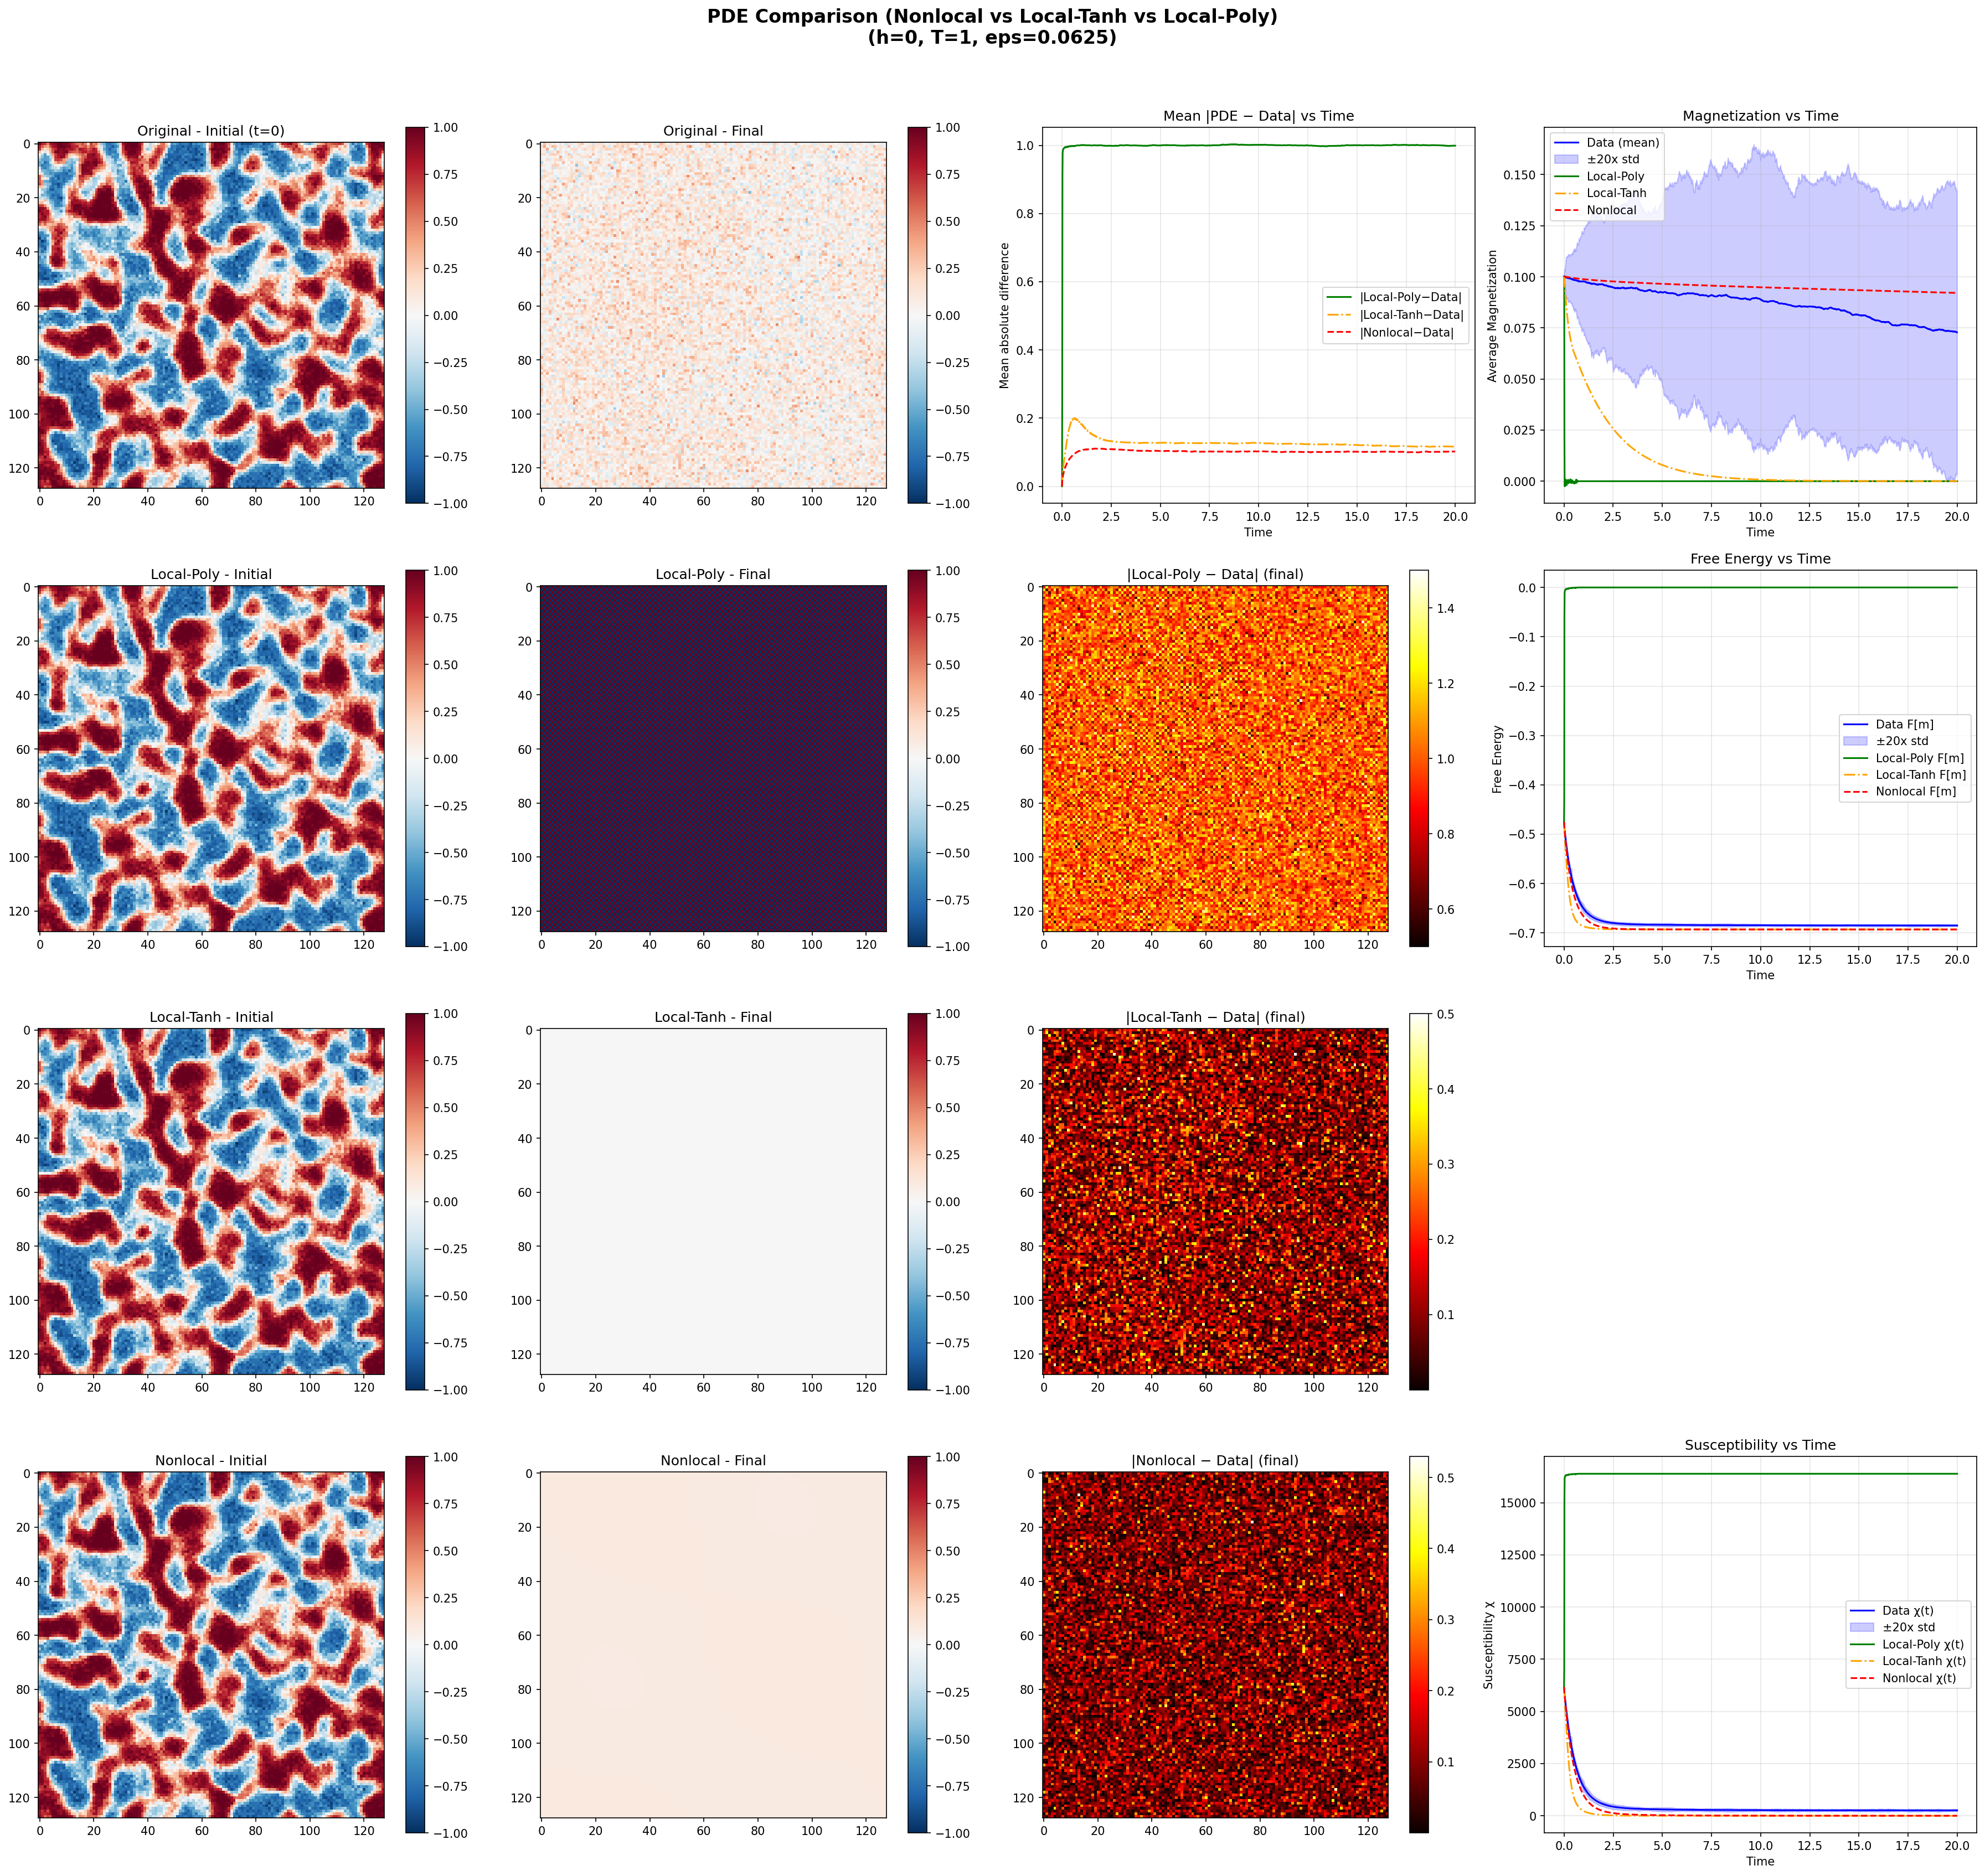
\includegraphics[width=1.0\textwidth]{fig/compare_pde_solvers_L1024_h0_T1_eps0.0625.png}
% 	\caption{Comparison of original data and PDE solutions for $h=0$, $T=1$, $\epsilon=0.0625$, $L=1024$.}
% 	\label{fig:pde_comparison_h0_T1_eps0.0625}
% \end{figure}

% \begin{figure}[!h]
% 	\centering
% 	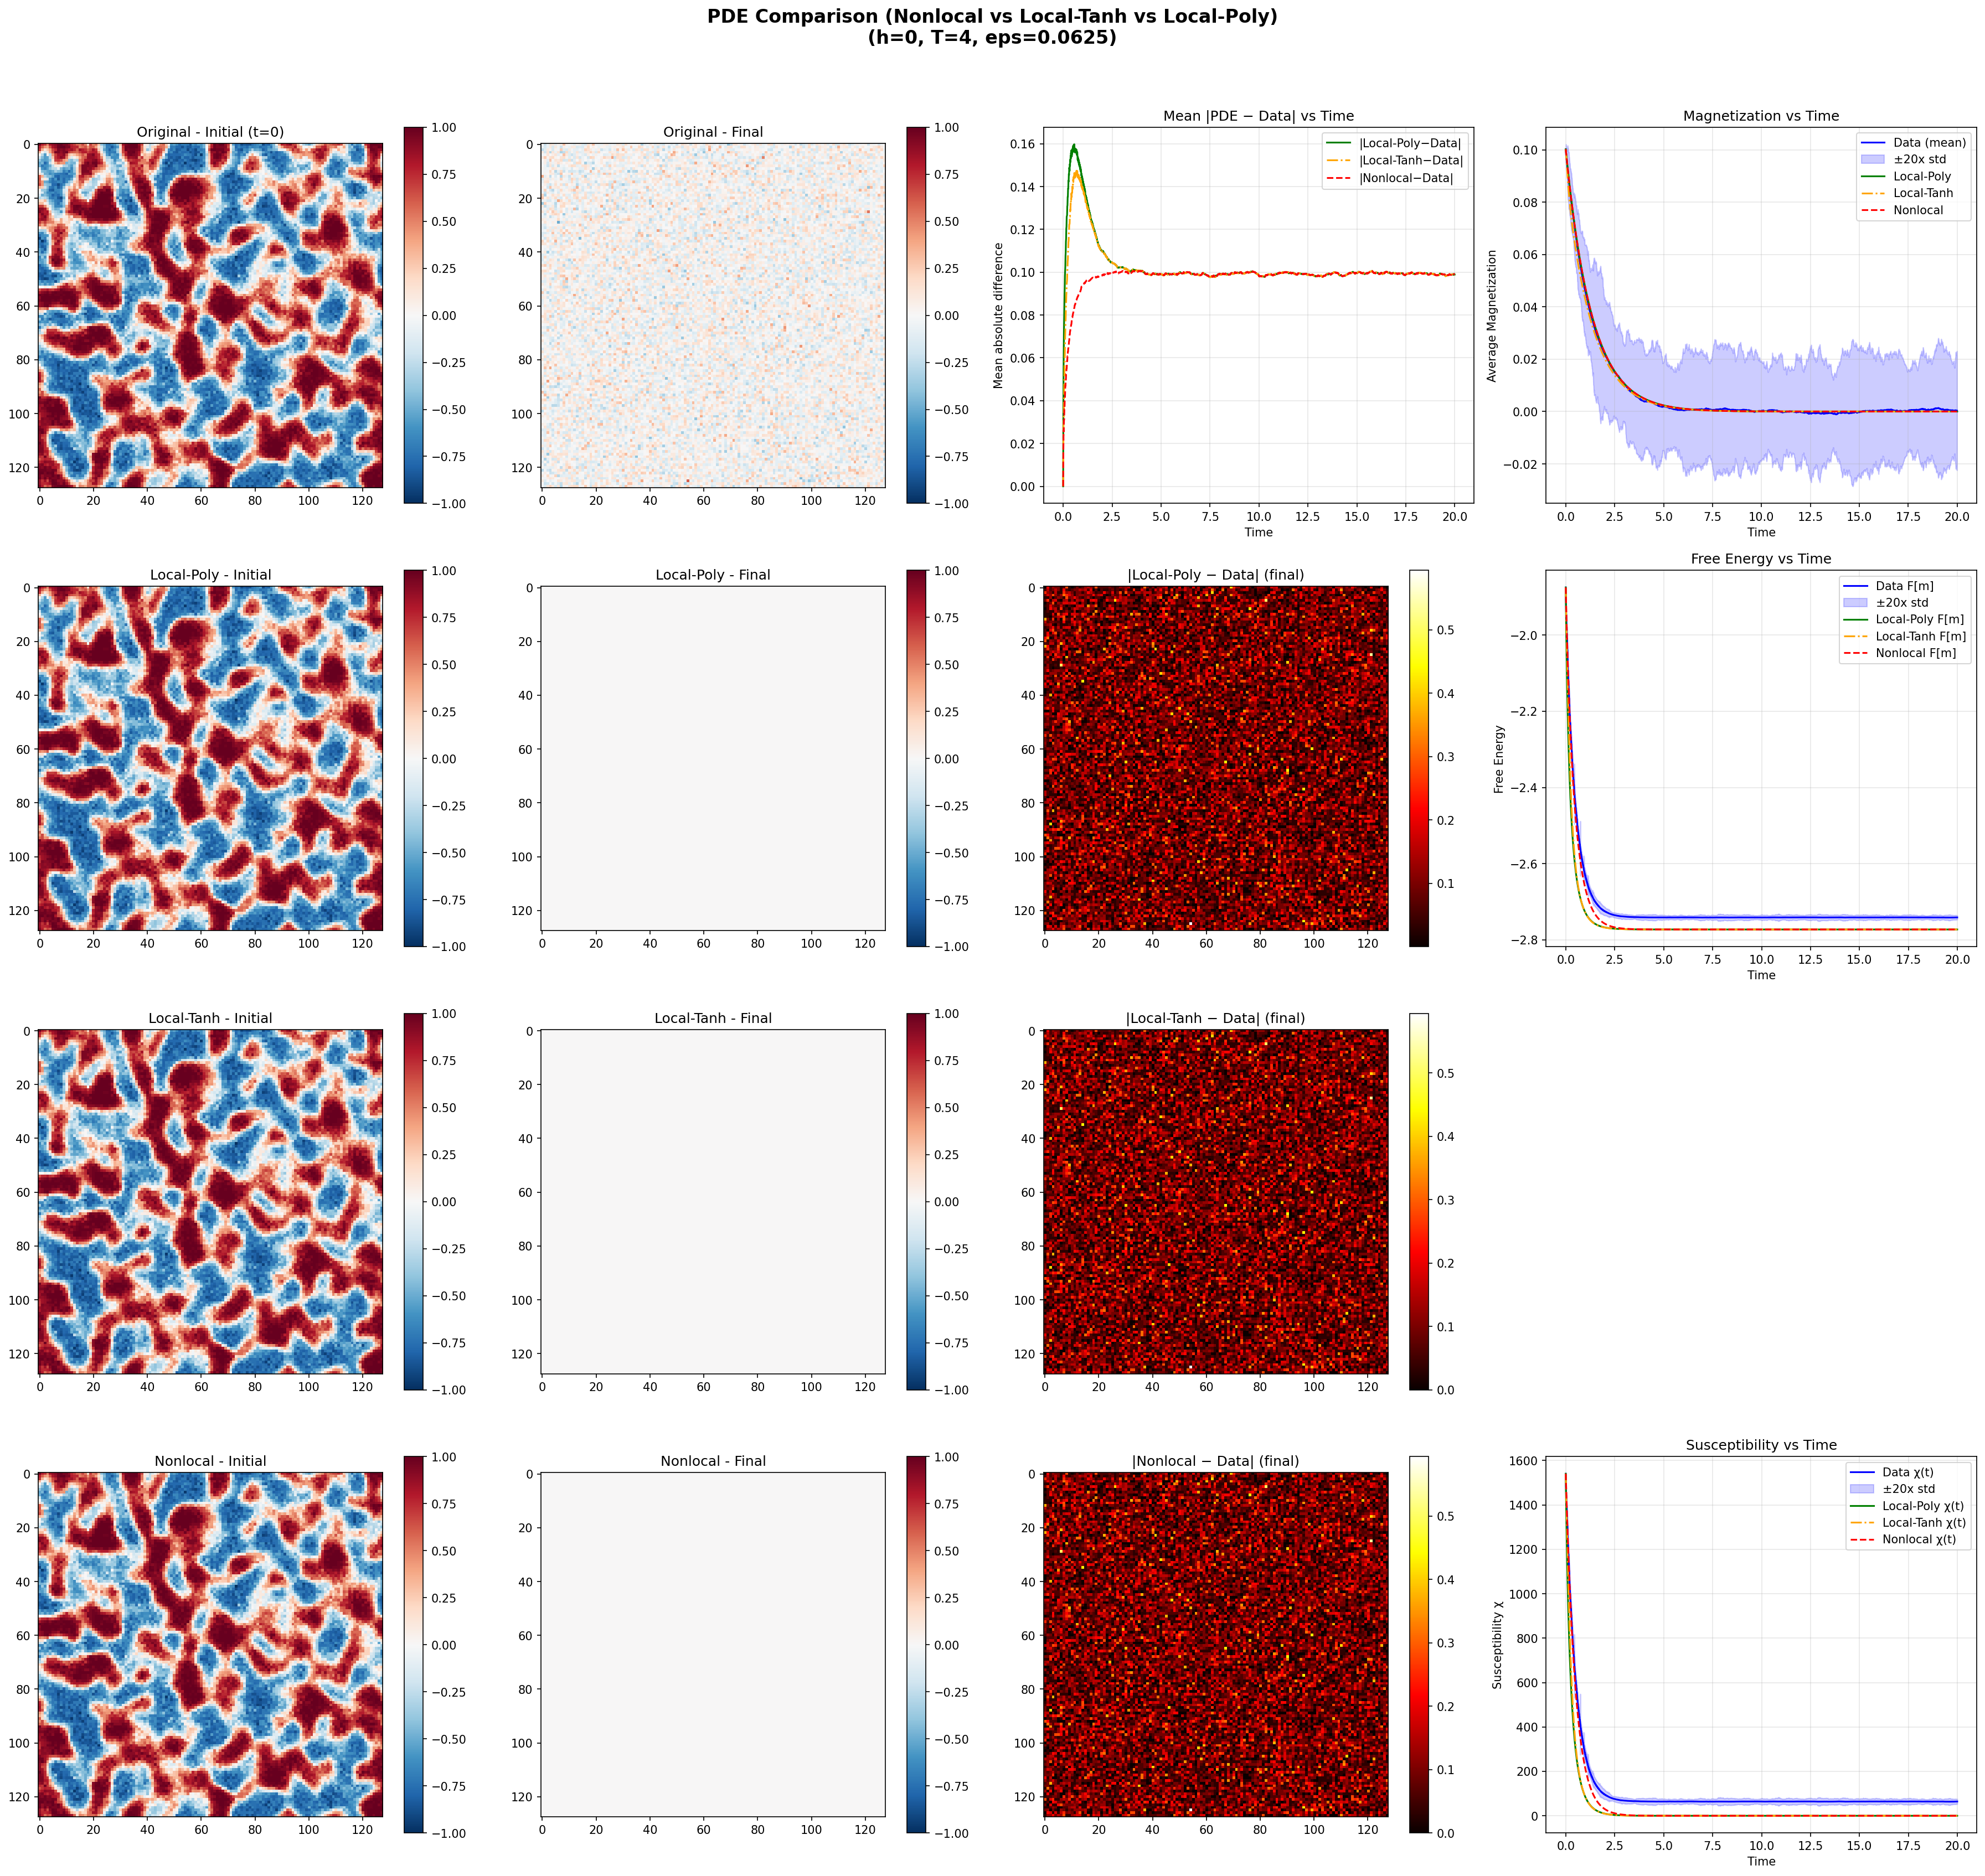
\includegraphics[width=1.0\textwidth]{fig/compare_pde_solvers_L1024_h0_T4_eps0.0625.png}
% 	\caption{Comparison of original data and PDE solutions for $h=0$, $T=4$, $\epsilon=0.0625$, $L=1024$.}
% 	\label{fig:pde_comparison_h0_T4_eps0.0625}
% \end{figure}

% \begin{figure}[!h]
% 	\centering
% 	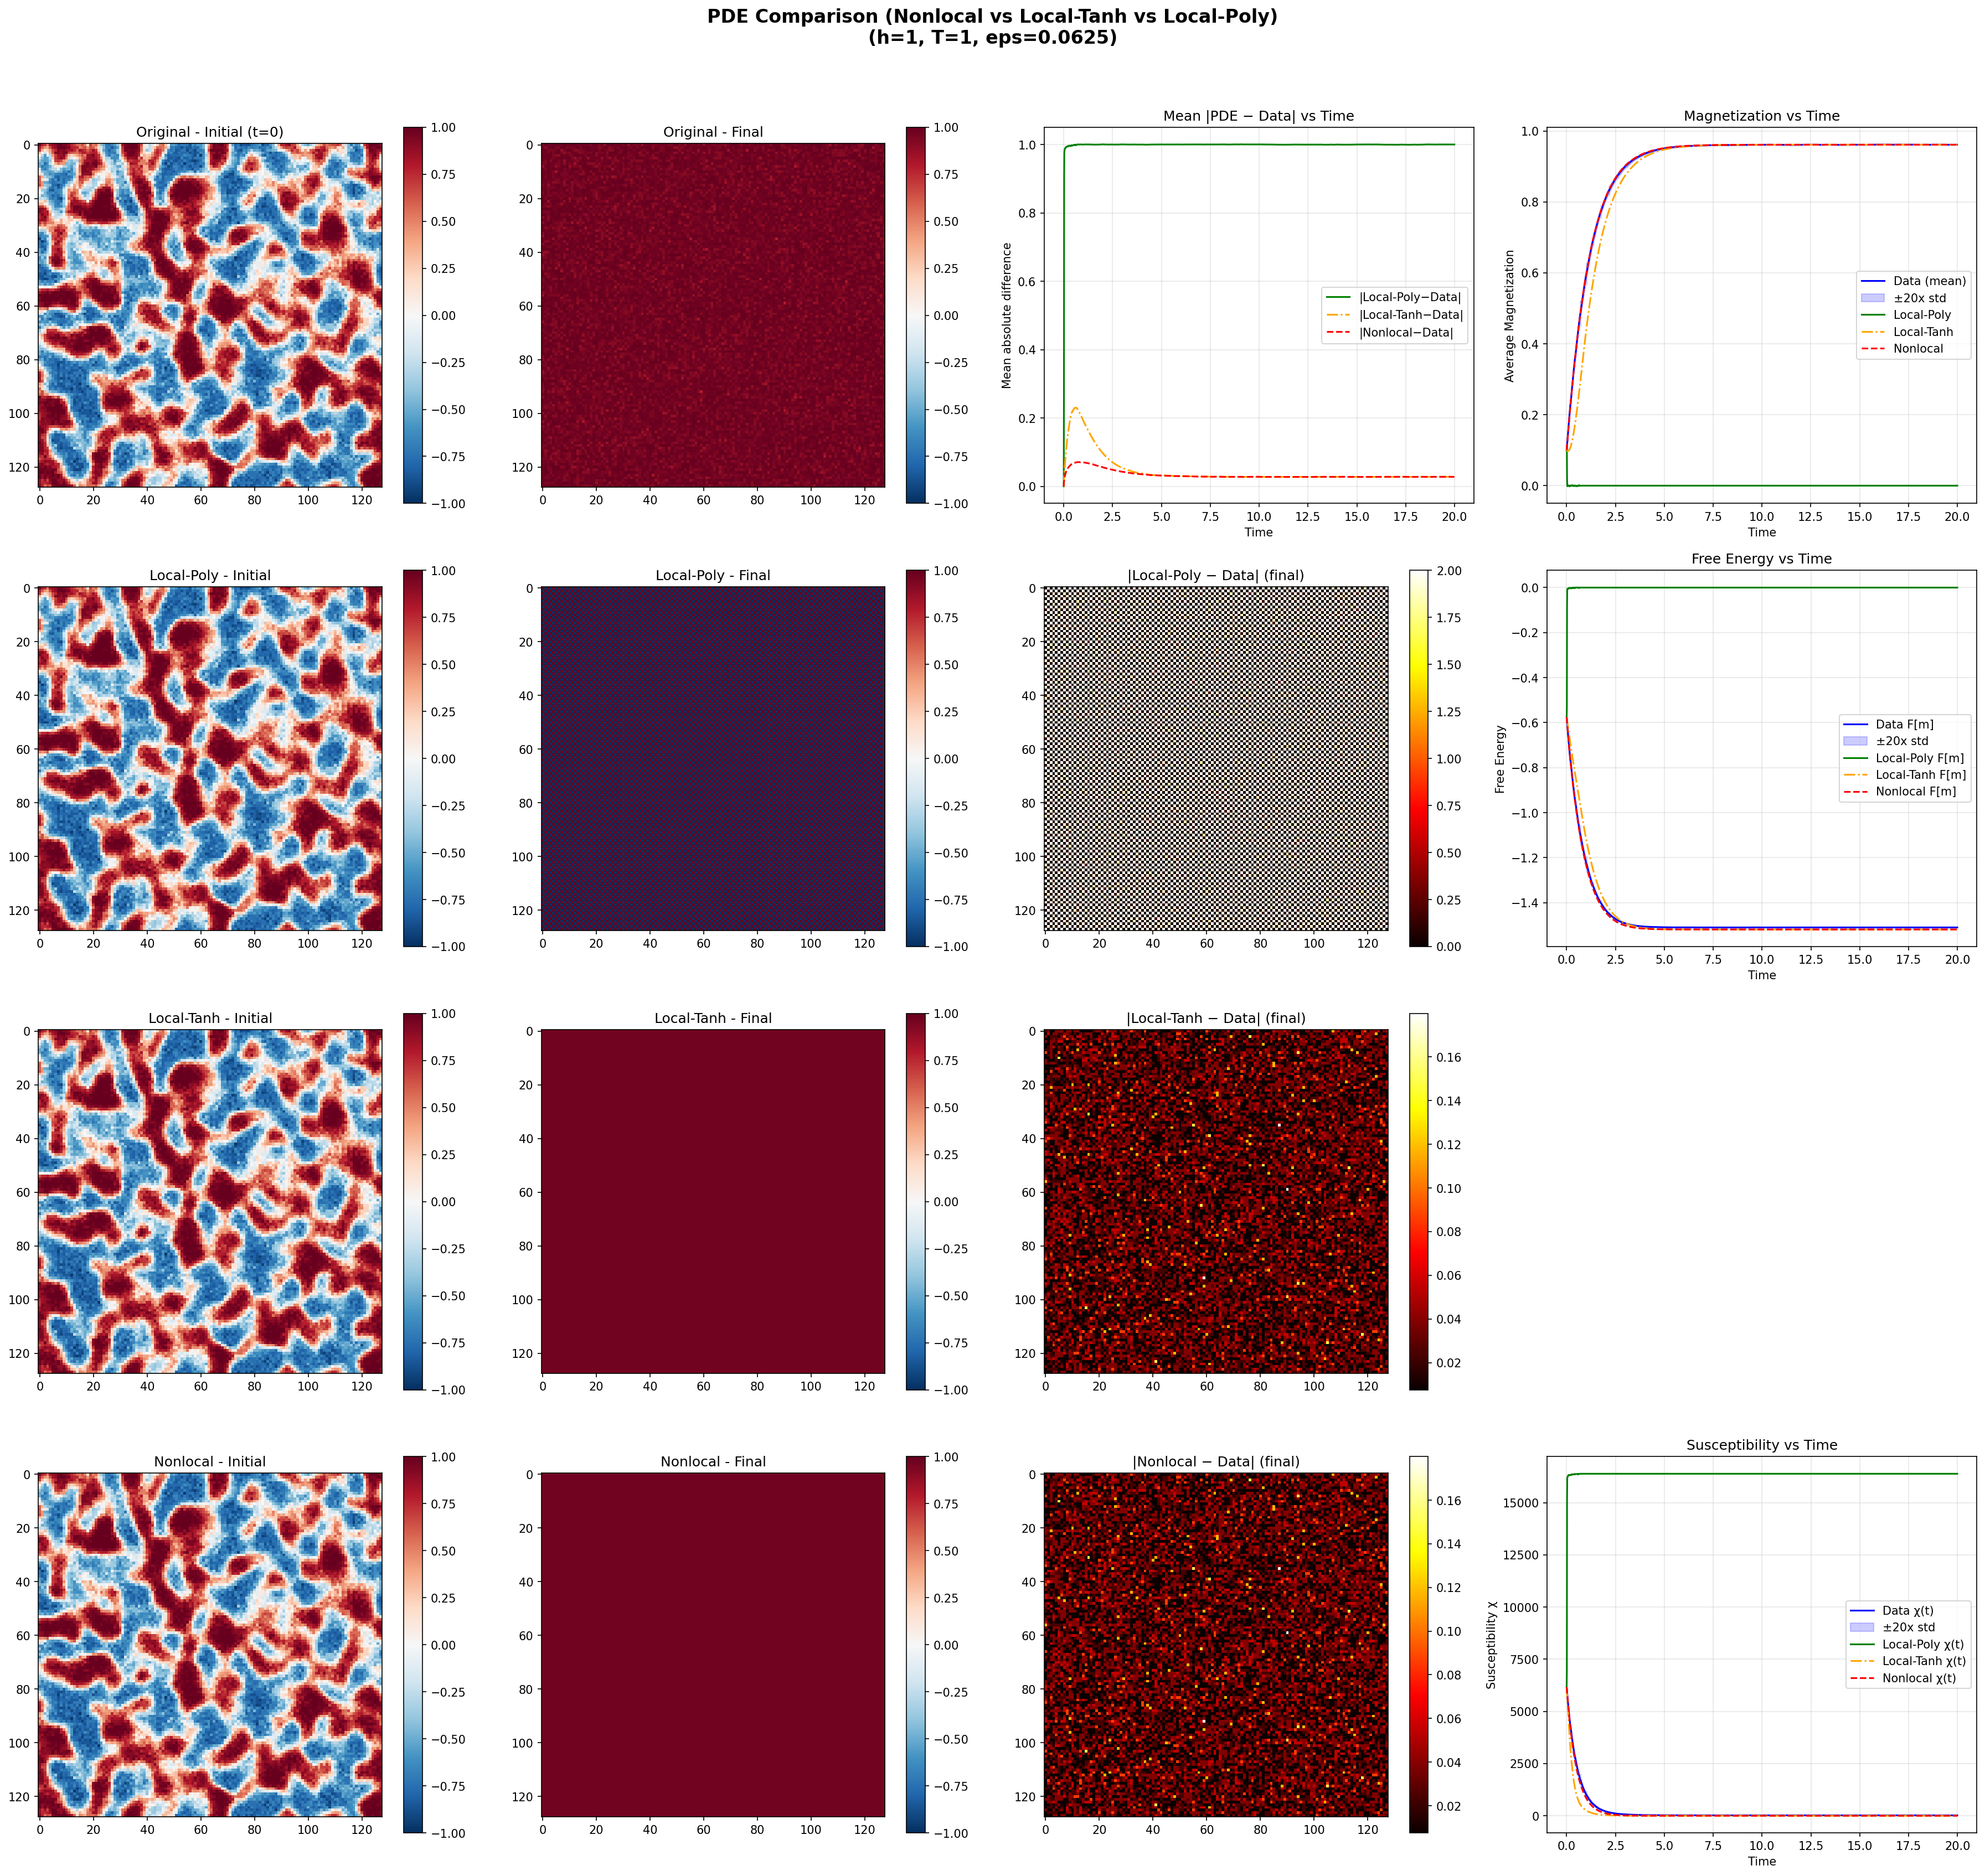
\includegraphics[width=1.0\textwidth]{fig/compare_pde_solvers_L1024_h1_T1_eps0.0625.png}
% 	\caption{Comparison of original data and PDE solutions for $h=1$, $T=1$, $\epsilon=0.0625$, $L=1024$.}
% 	\label{fig:pde_comparison_h1_T1_eps0.0625}
% \end{figure}

% \begin{figure}[!h]
% 	\centering
% 	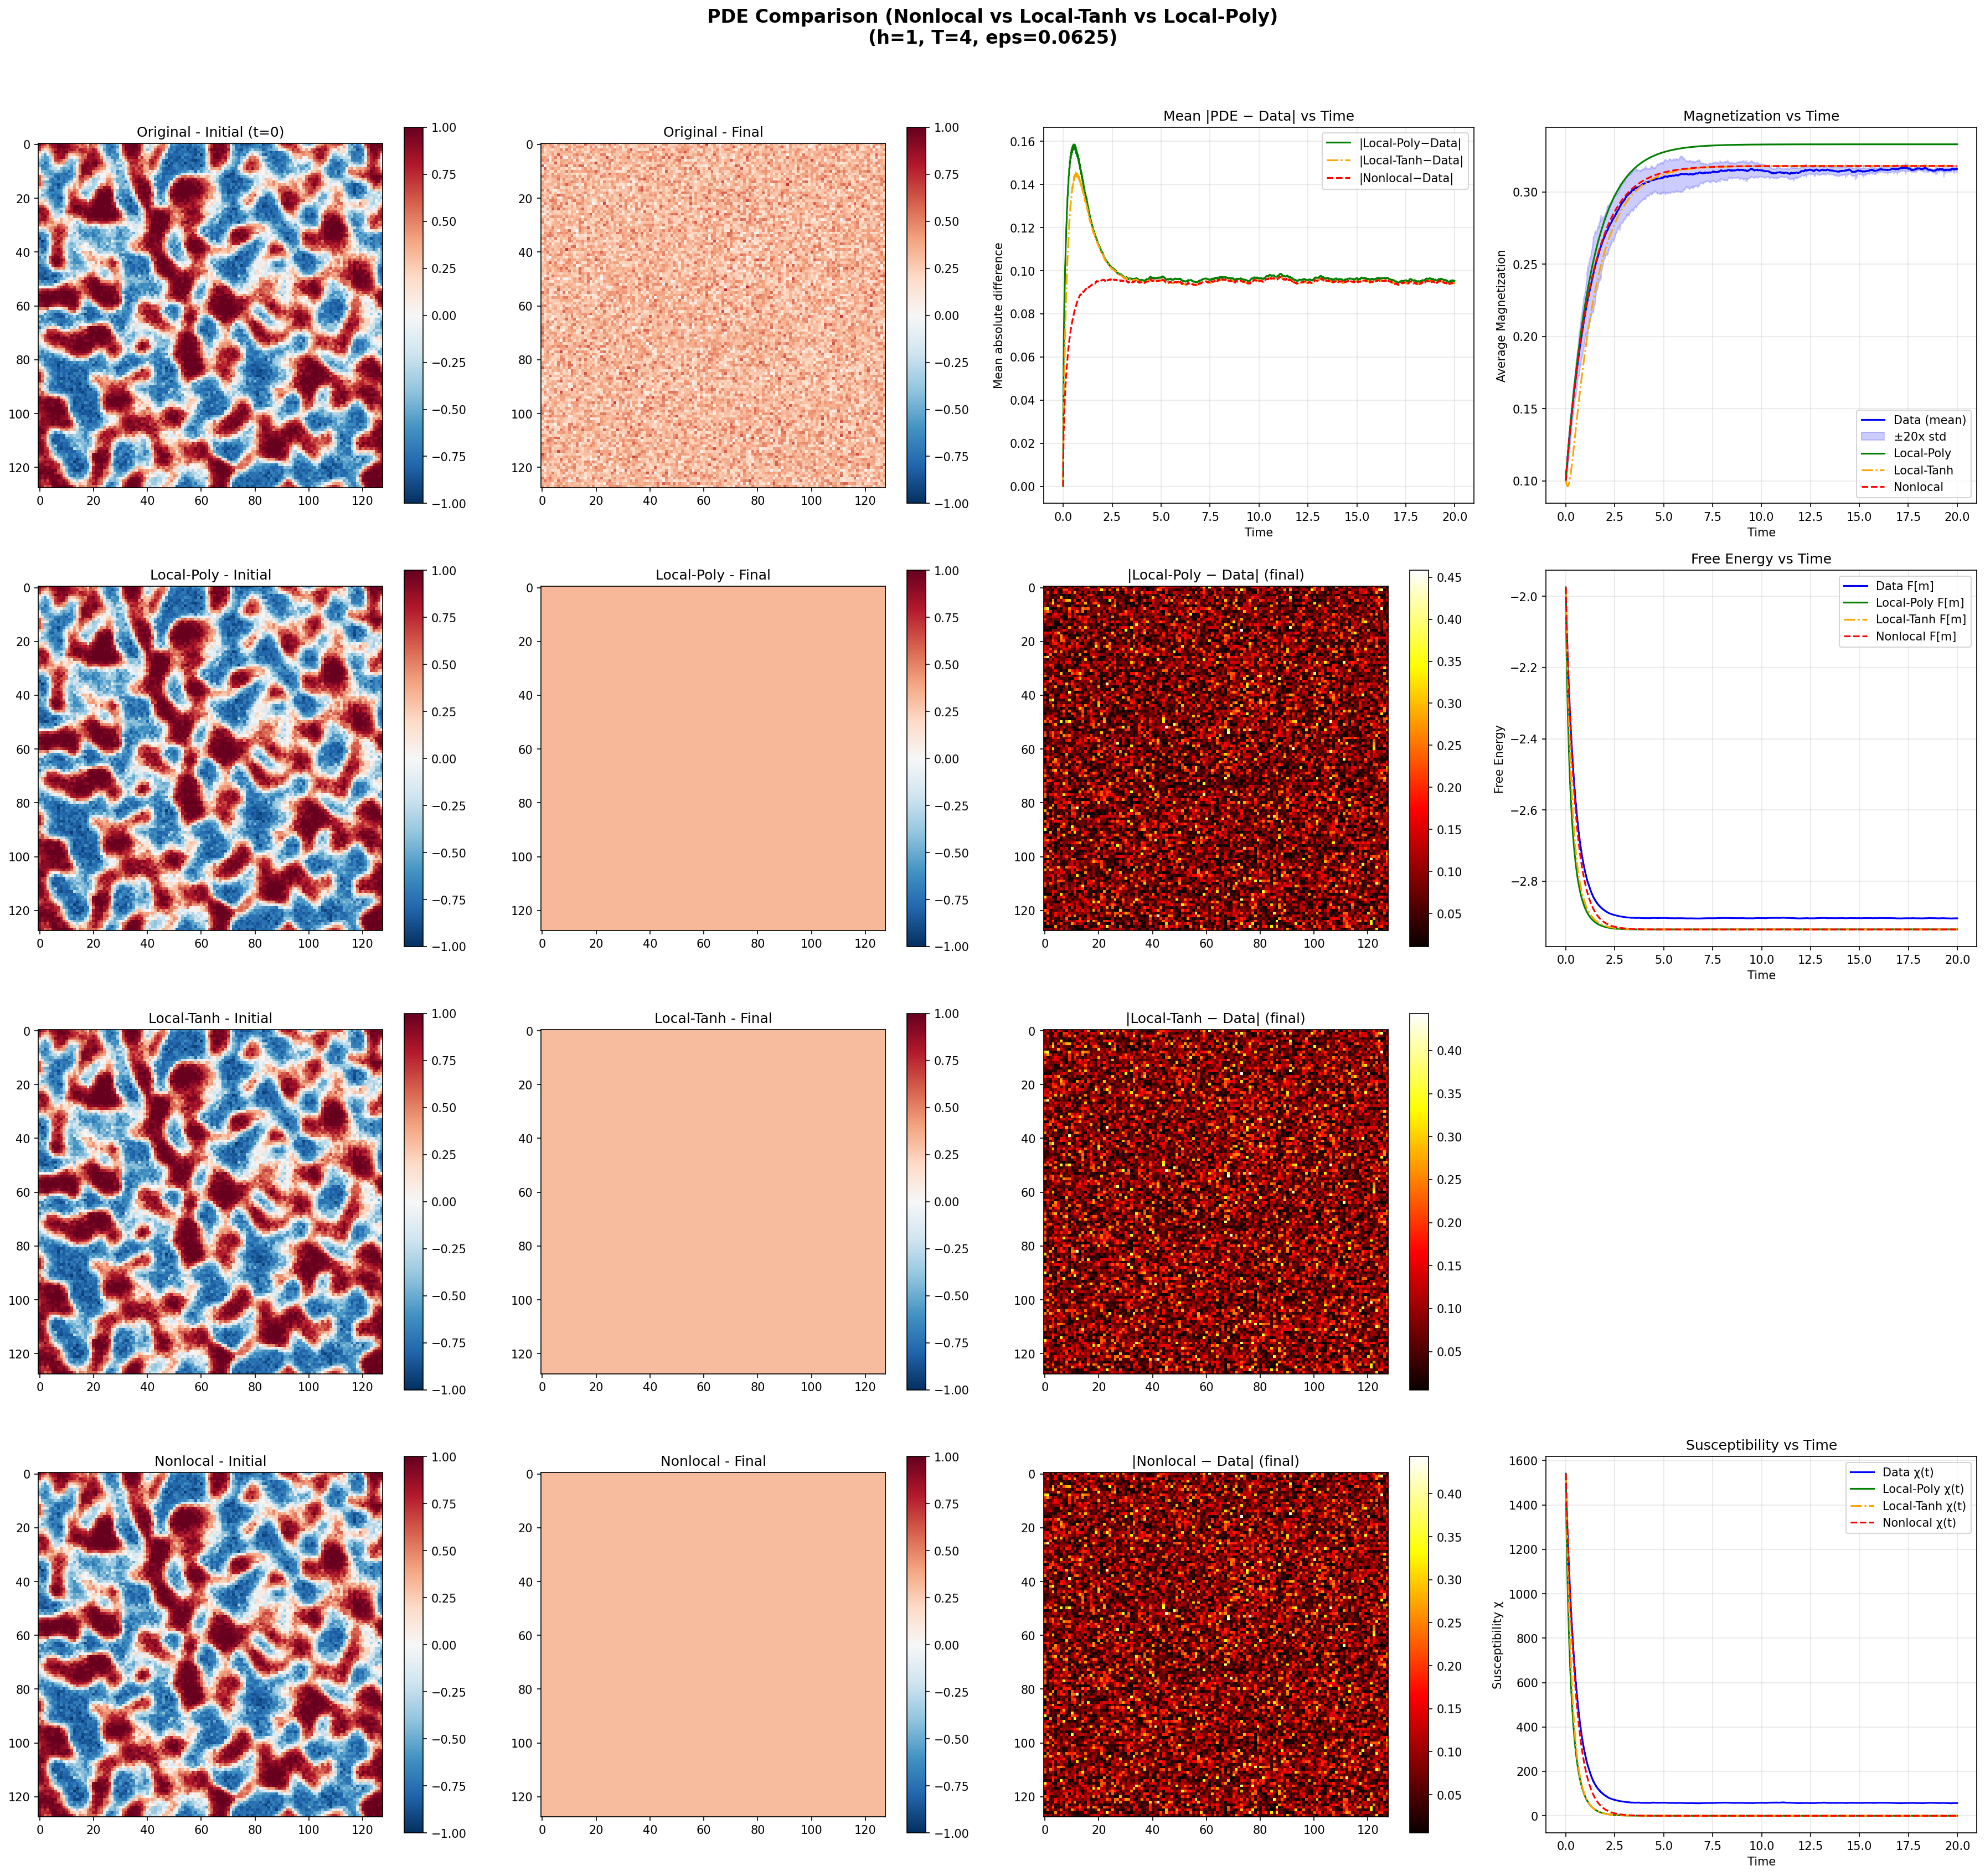
\includegraphics[width=1.0\textwidth]{fig/compare_pde_solvers_L1024_h1_T4_eps0.0625.png}
% 	\caption{Comparison of original data and PDE solutions for $h=1$, $T=4$, $\epsilon=0.0625$, $L=1024$.}
% 	\label{fig:pde_comparison_h1_T4_eps0.0625}
% \end{figure}


% % with epsilon = 0.015625, L = 2048

% \begin{figure}[!h]
% 	\centering
% 	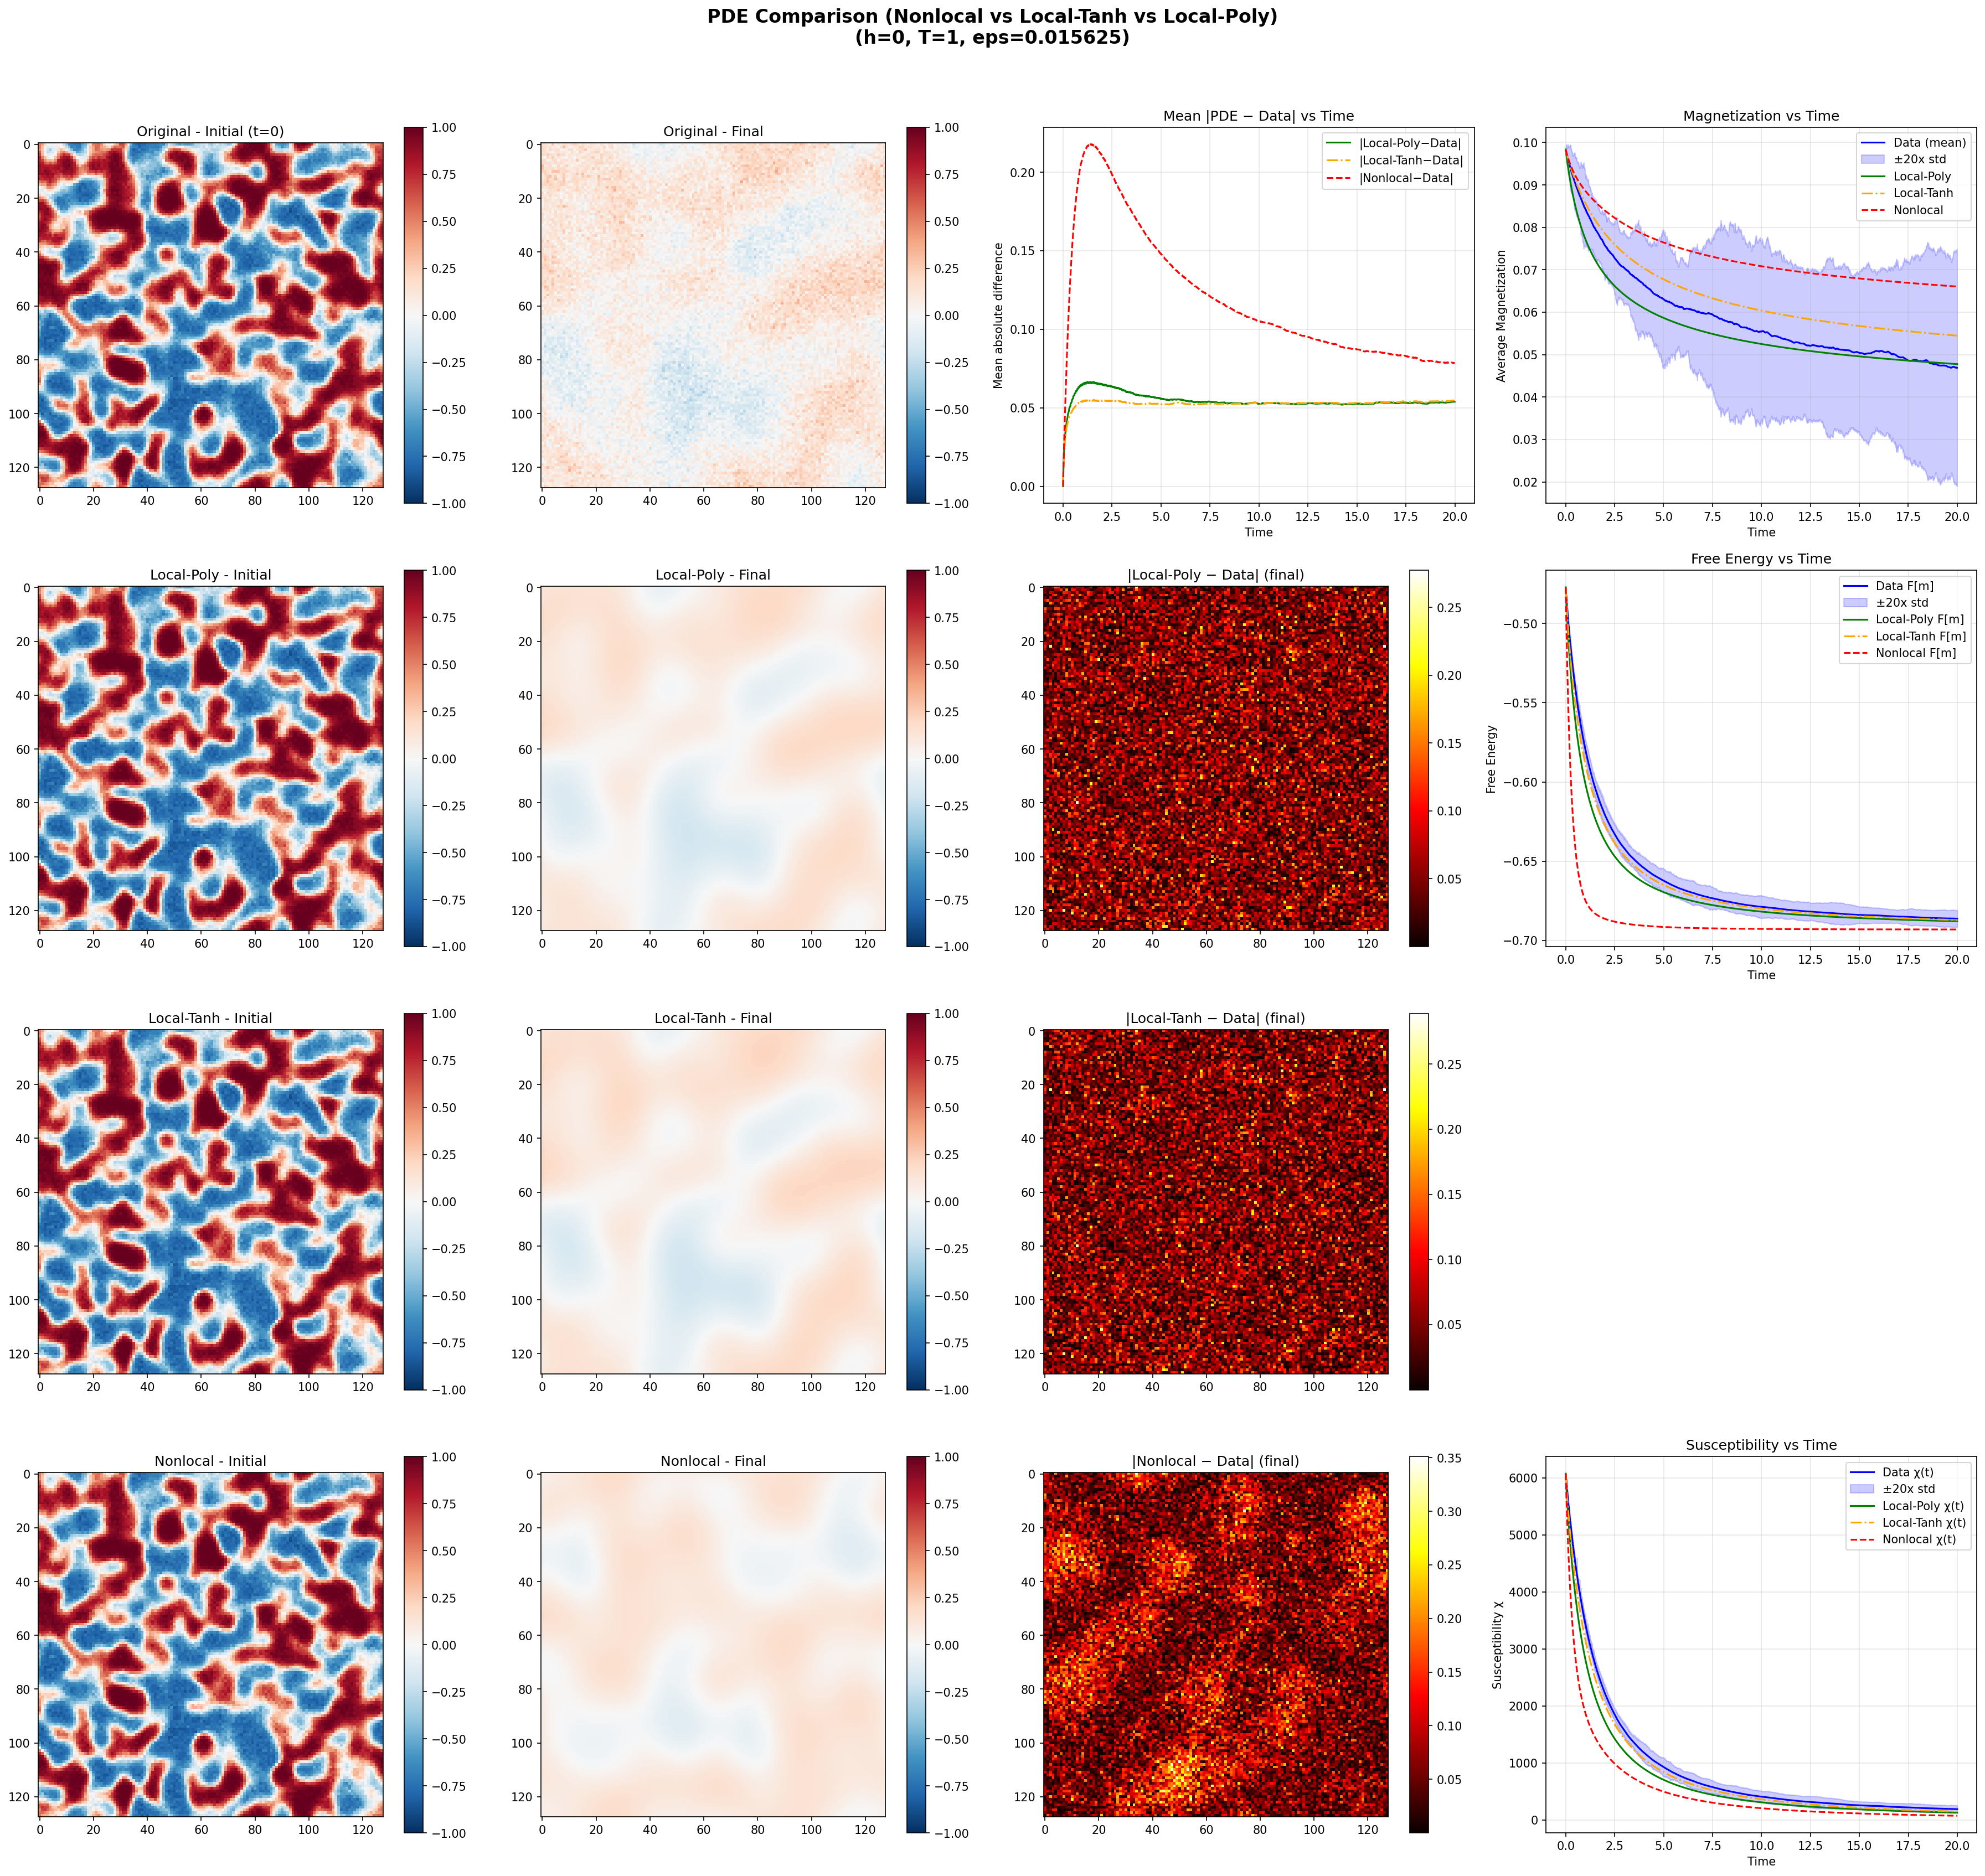
\includegraphics[width=1.0\textwidth]{fig/compare_pde_solvers_L2048_h0_T1_eps0.015625.png}
% 	\caption{Comparison of original data and PDE solutions for $h=0$, $T=1$, $\epsilon=0.015625$, $L=2048$.}
% 	\label{fig:pde_comparison_h0_T1_eps0.015625_L2048}
% \end{figure}


% \begin{figure}[!h]
% 	\centering
% 	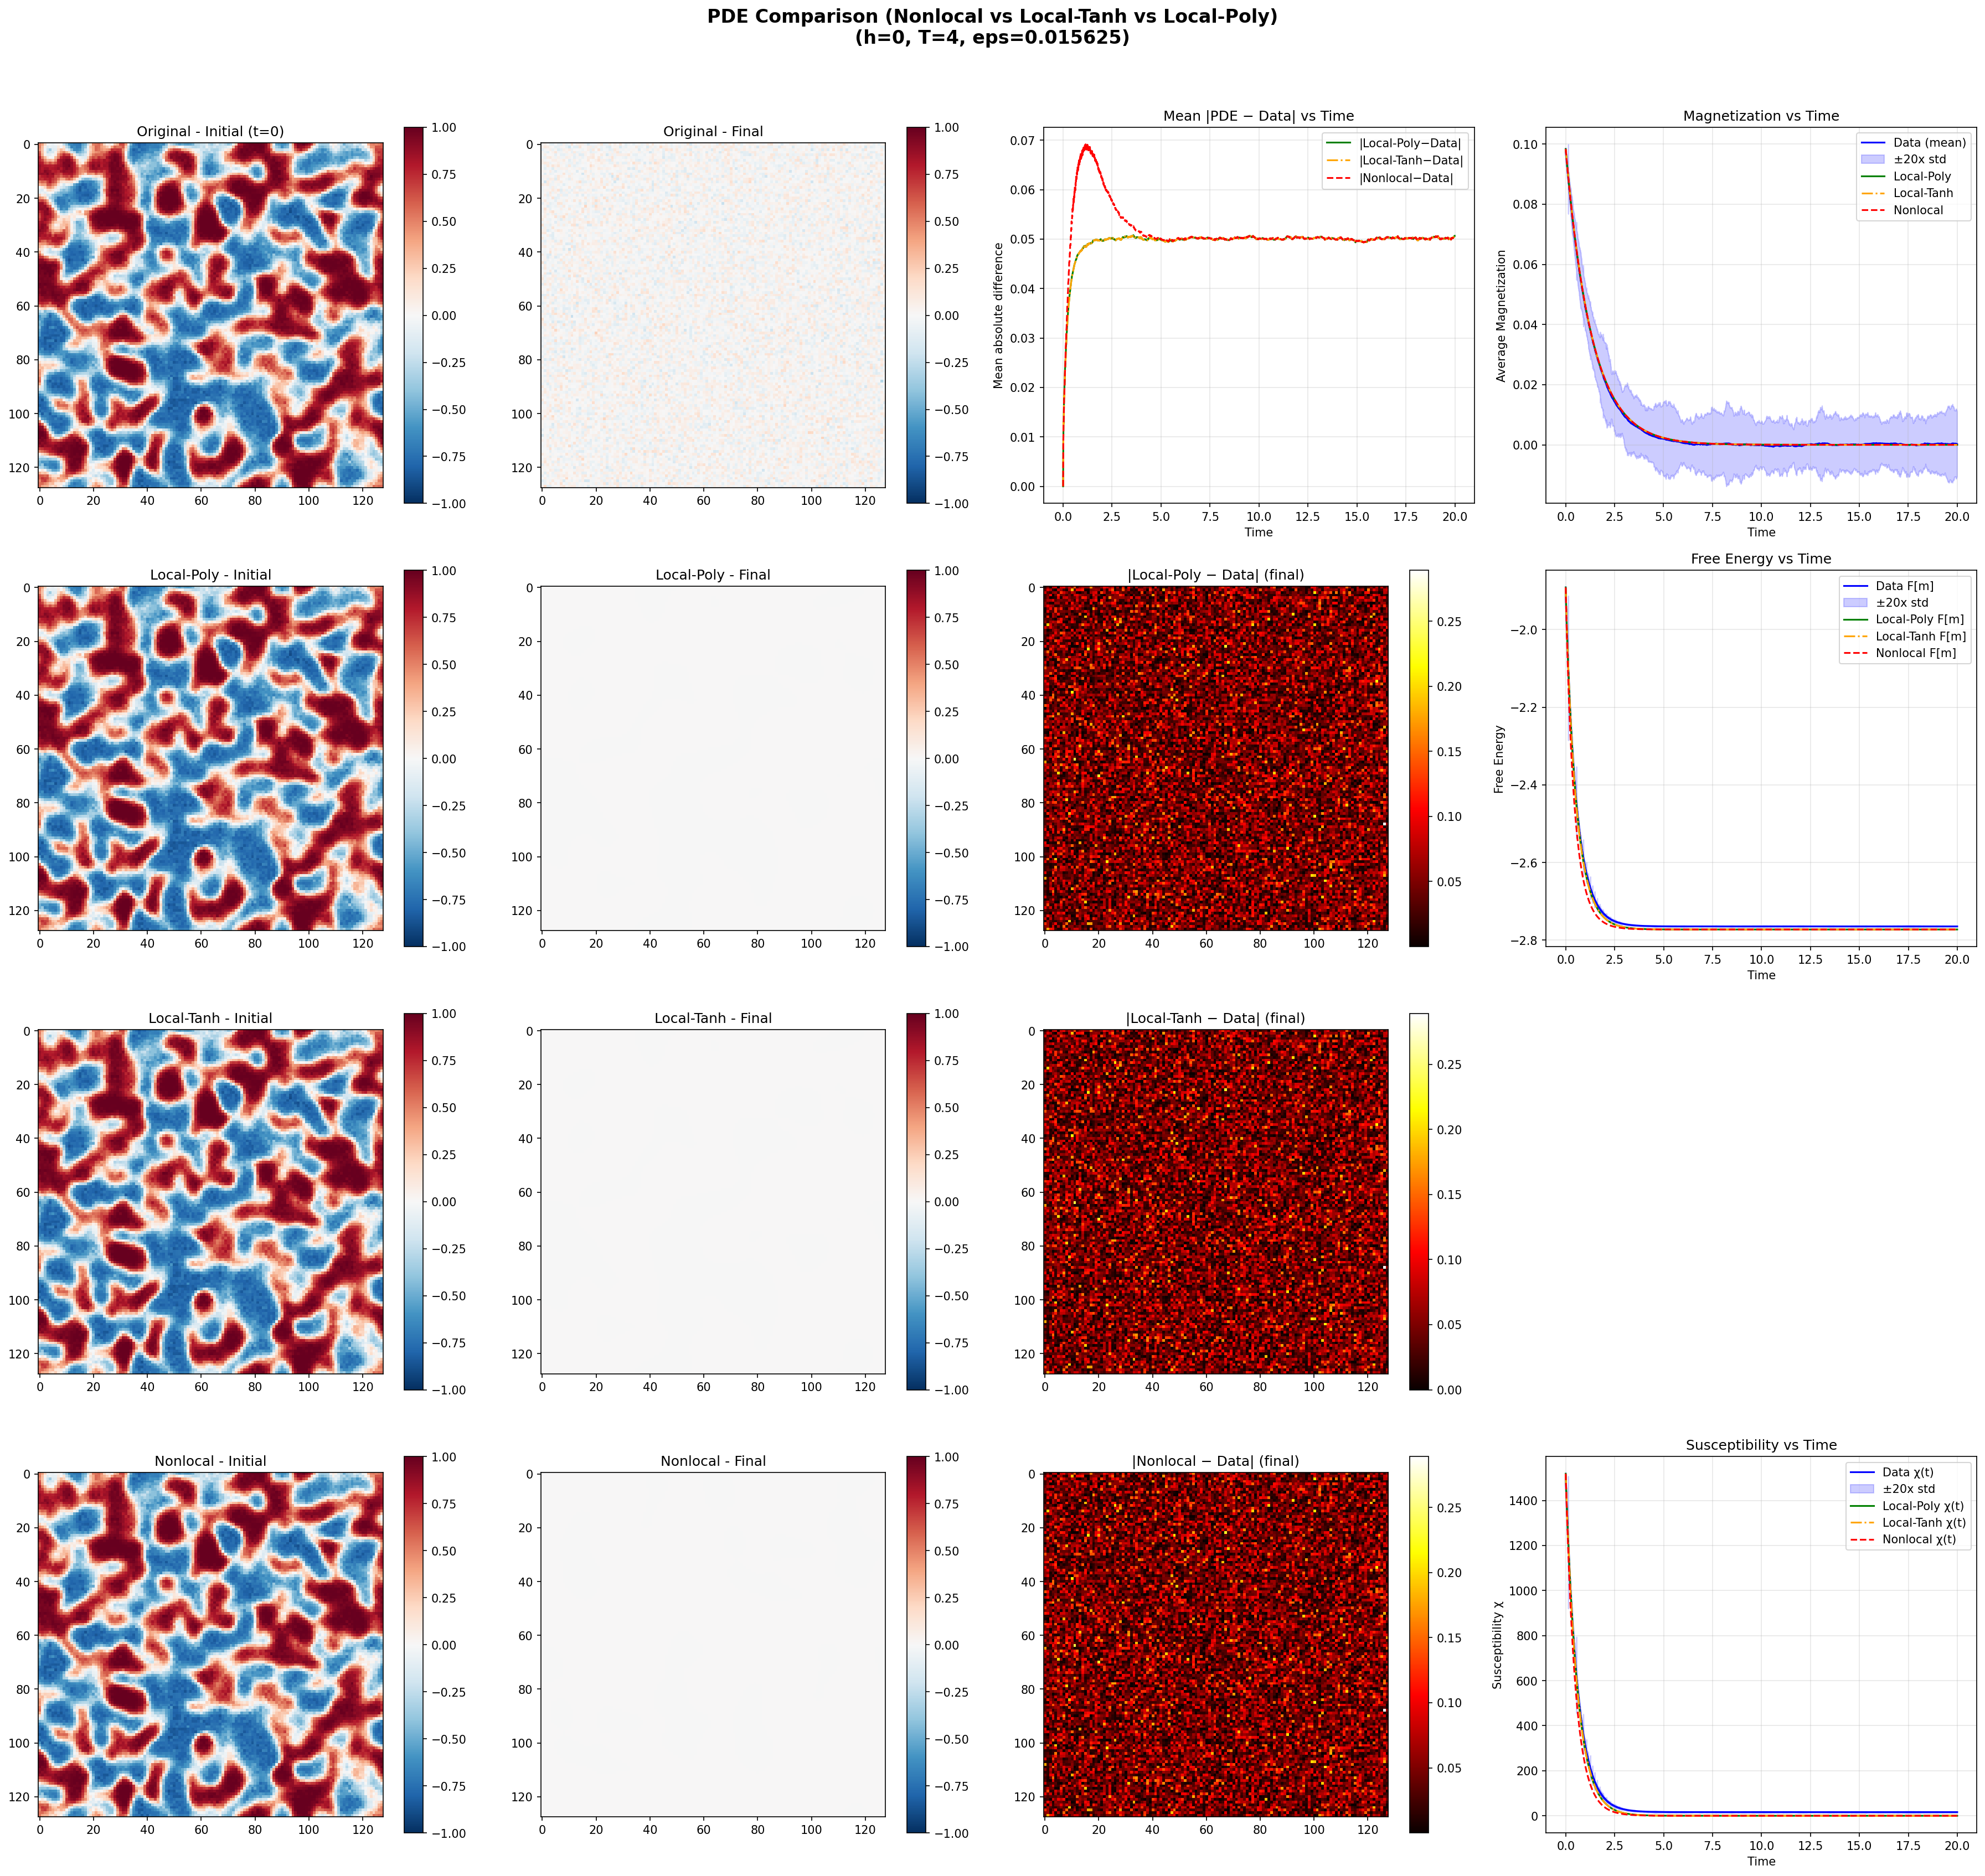
\includegraphics[width=1.0\textwidth]{fig/compare_pde_solvers_L2048_h0_T4_eps0.015625.png}
% 	\caption{Comparison of original data and PDE solutions for $h=0$, $T=4$, $\epsilon=0.015625$, $L=2048$.}
% 	\label{fig:pde_comparison_h0_T4_eps0.015625_L2048}
% \end{figure}


% \begin{figure}[!h]
% 	\centering
% 	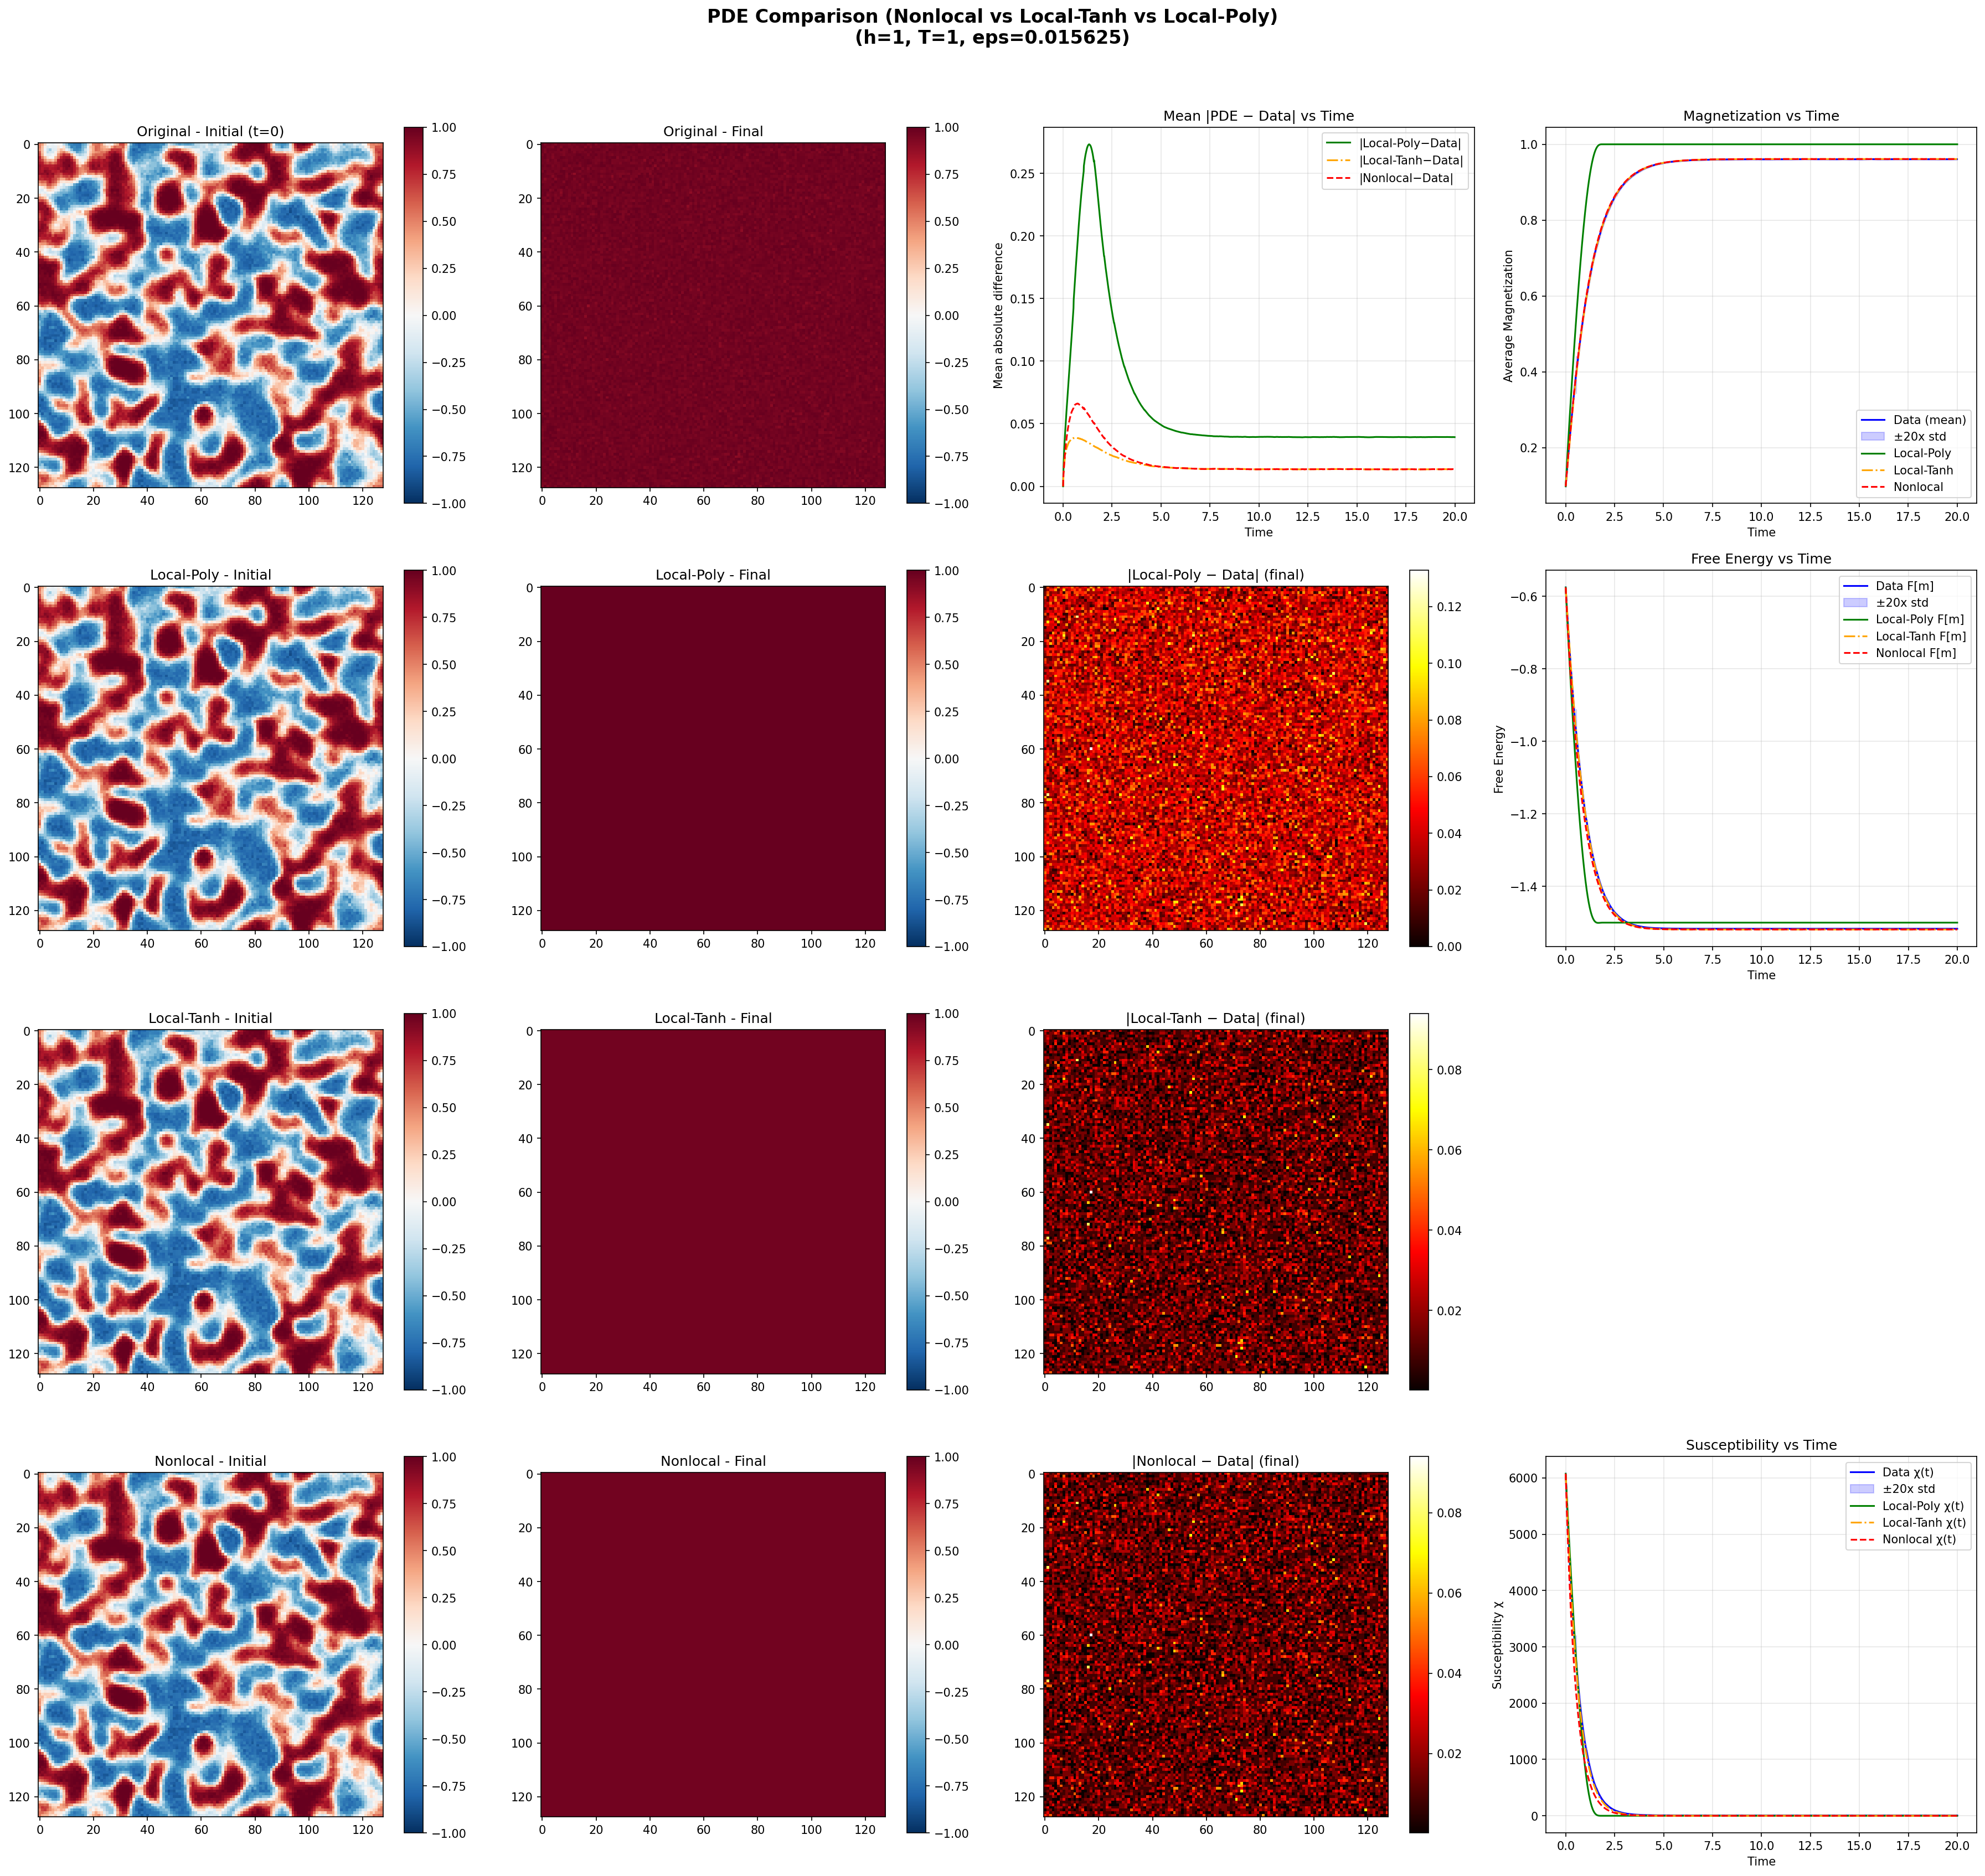
\includegraphics[width=1.0\textwidth]{fig/compare_pde_solvers_L2048_h1_T1_eps0.015625.png}
% 	\caption{Comparison of original data and PDE solutions for $h=1$, $T=1$, $\epsilon=0.015625$, $L=2048$.}
% 	\label{fig:pde_comparison_h1_T1_eps0.015625_L2048}
% \end{figure}


% \begin{figure}[!h]
% 	\centering
% 	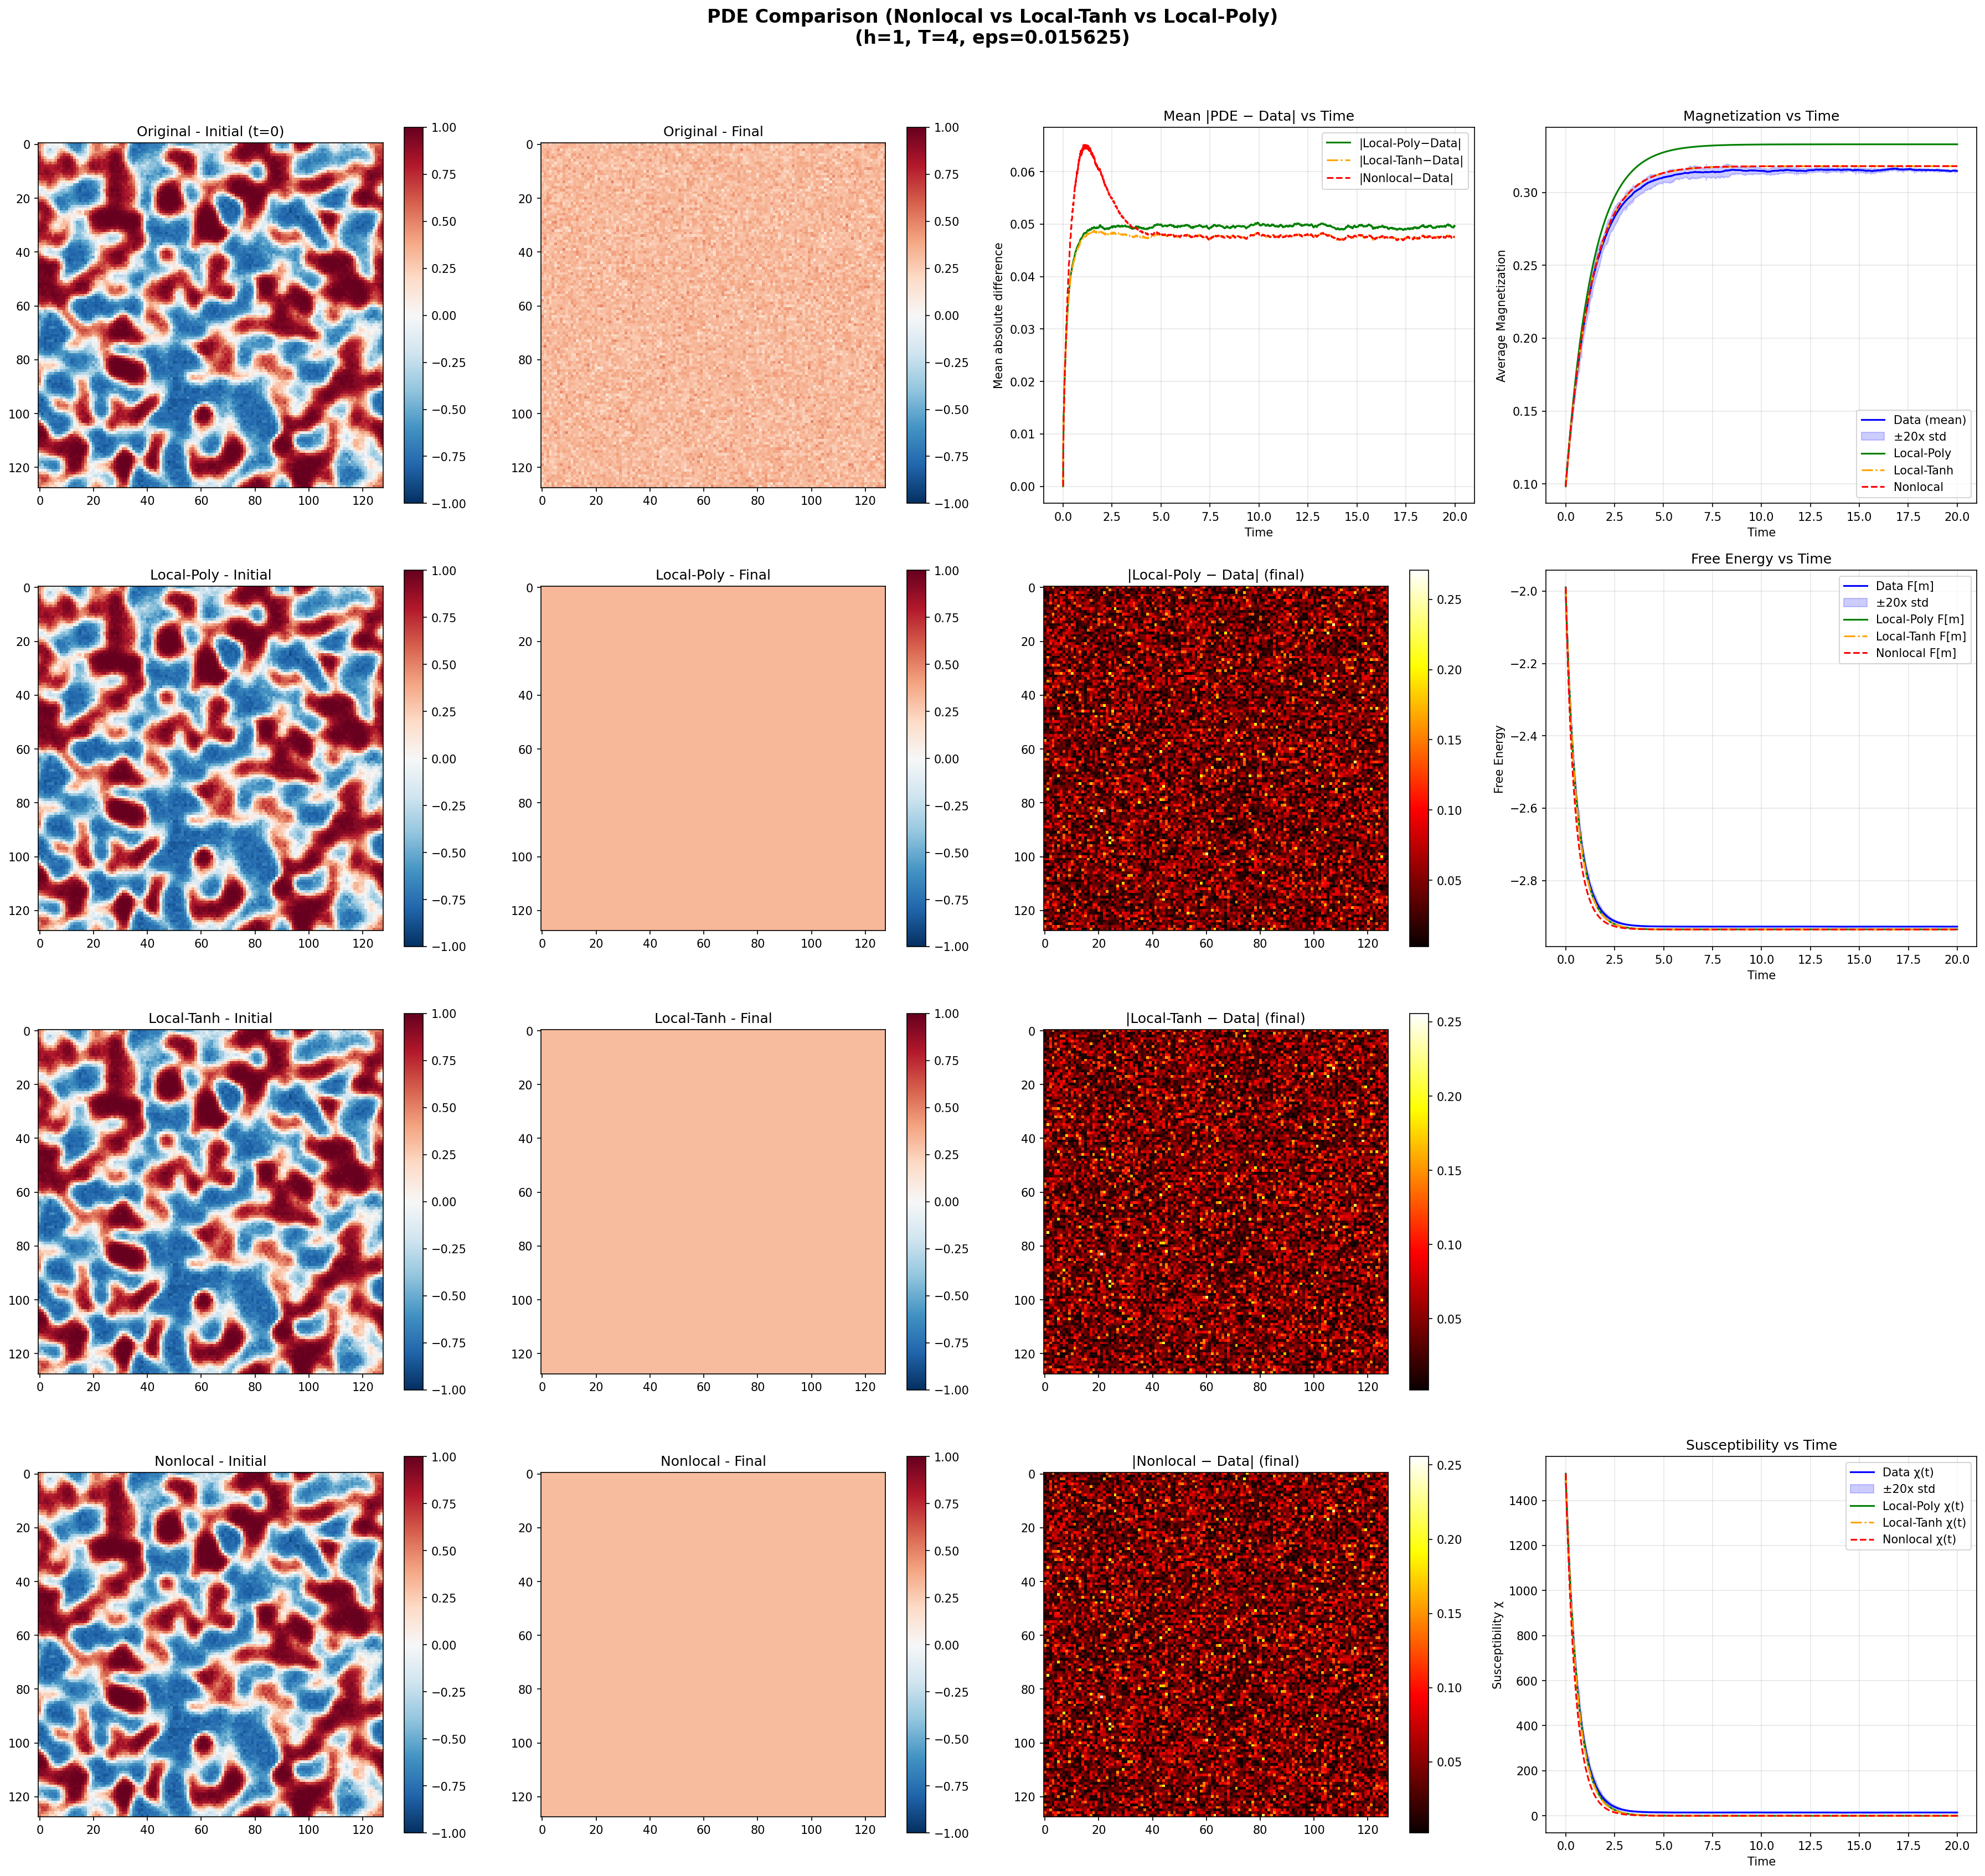
\includegraphics[width=1.0\textwidth]{fig/compare_pde_solvers_L2048_h1_T4_eps0.015625.png}
% 	\caption{Comparison of original data and PDE solutions for $h=1$, $T=4$, $\epsilon=0.015625$, $L=2048$.}
% 	\label{fig:pde_comparison_h1_T4_eps0.015625_L2048}
% \end{figure}

% % with epsilon = 0.03125

% \begin{figure}[!h]
% 	\centering
% 	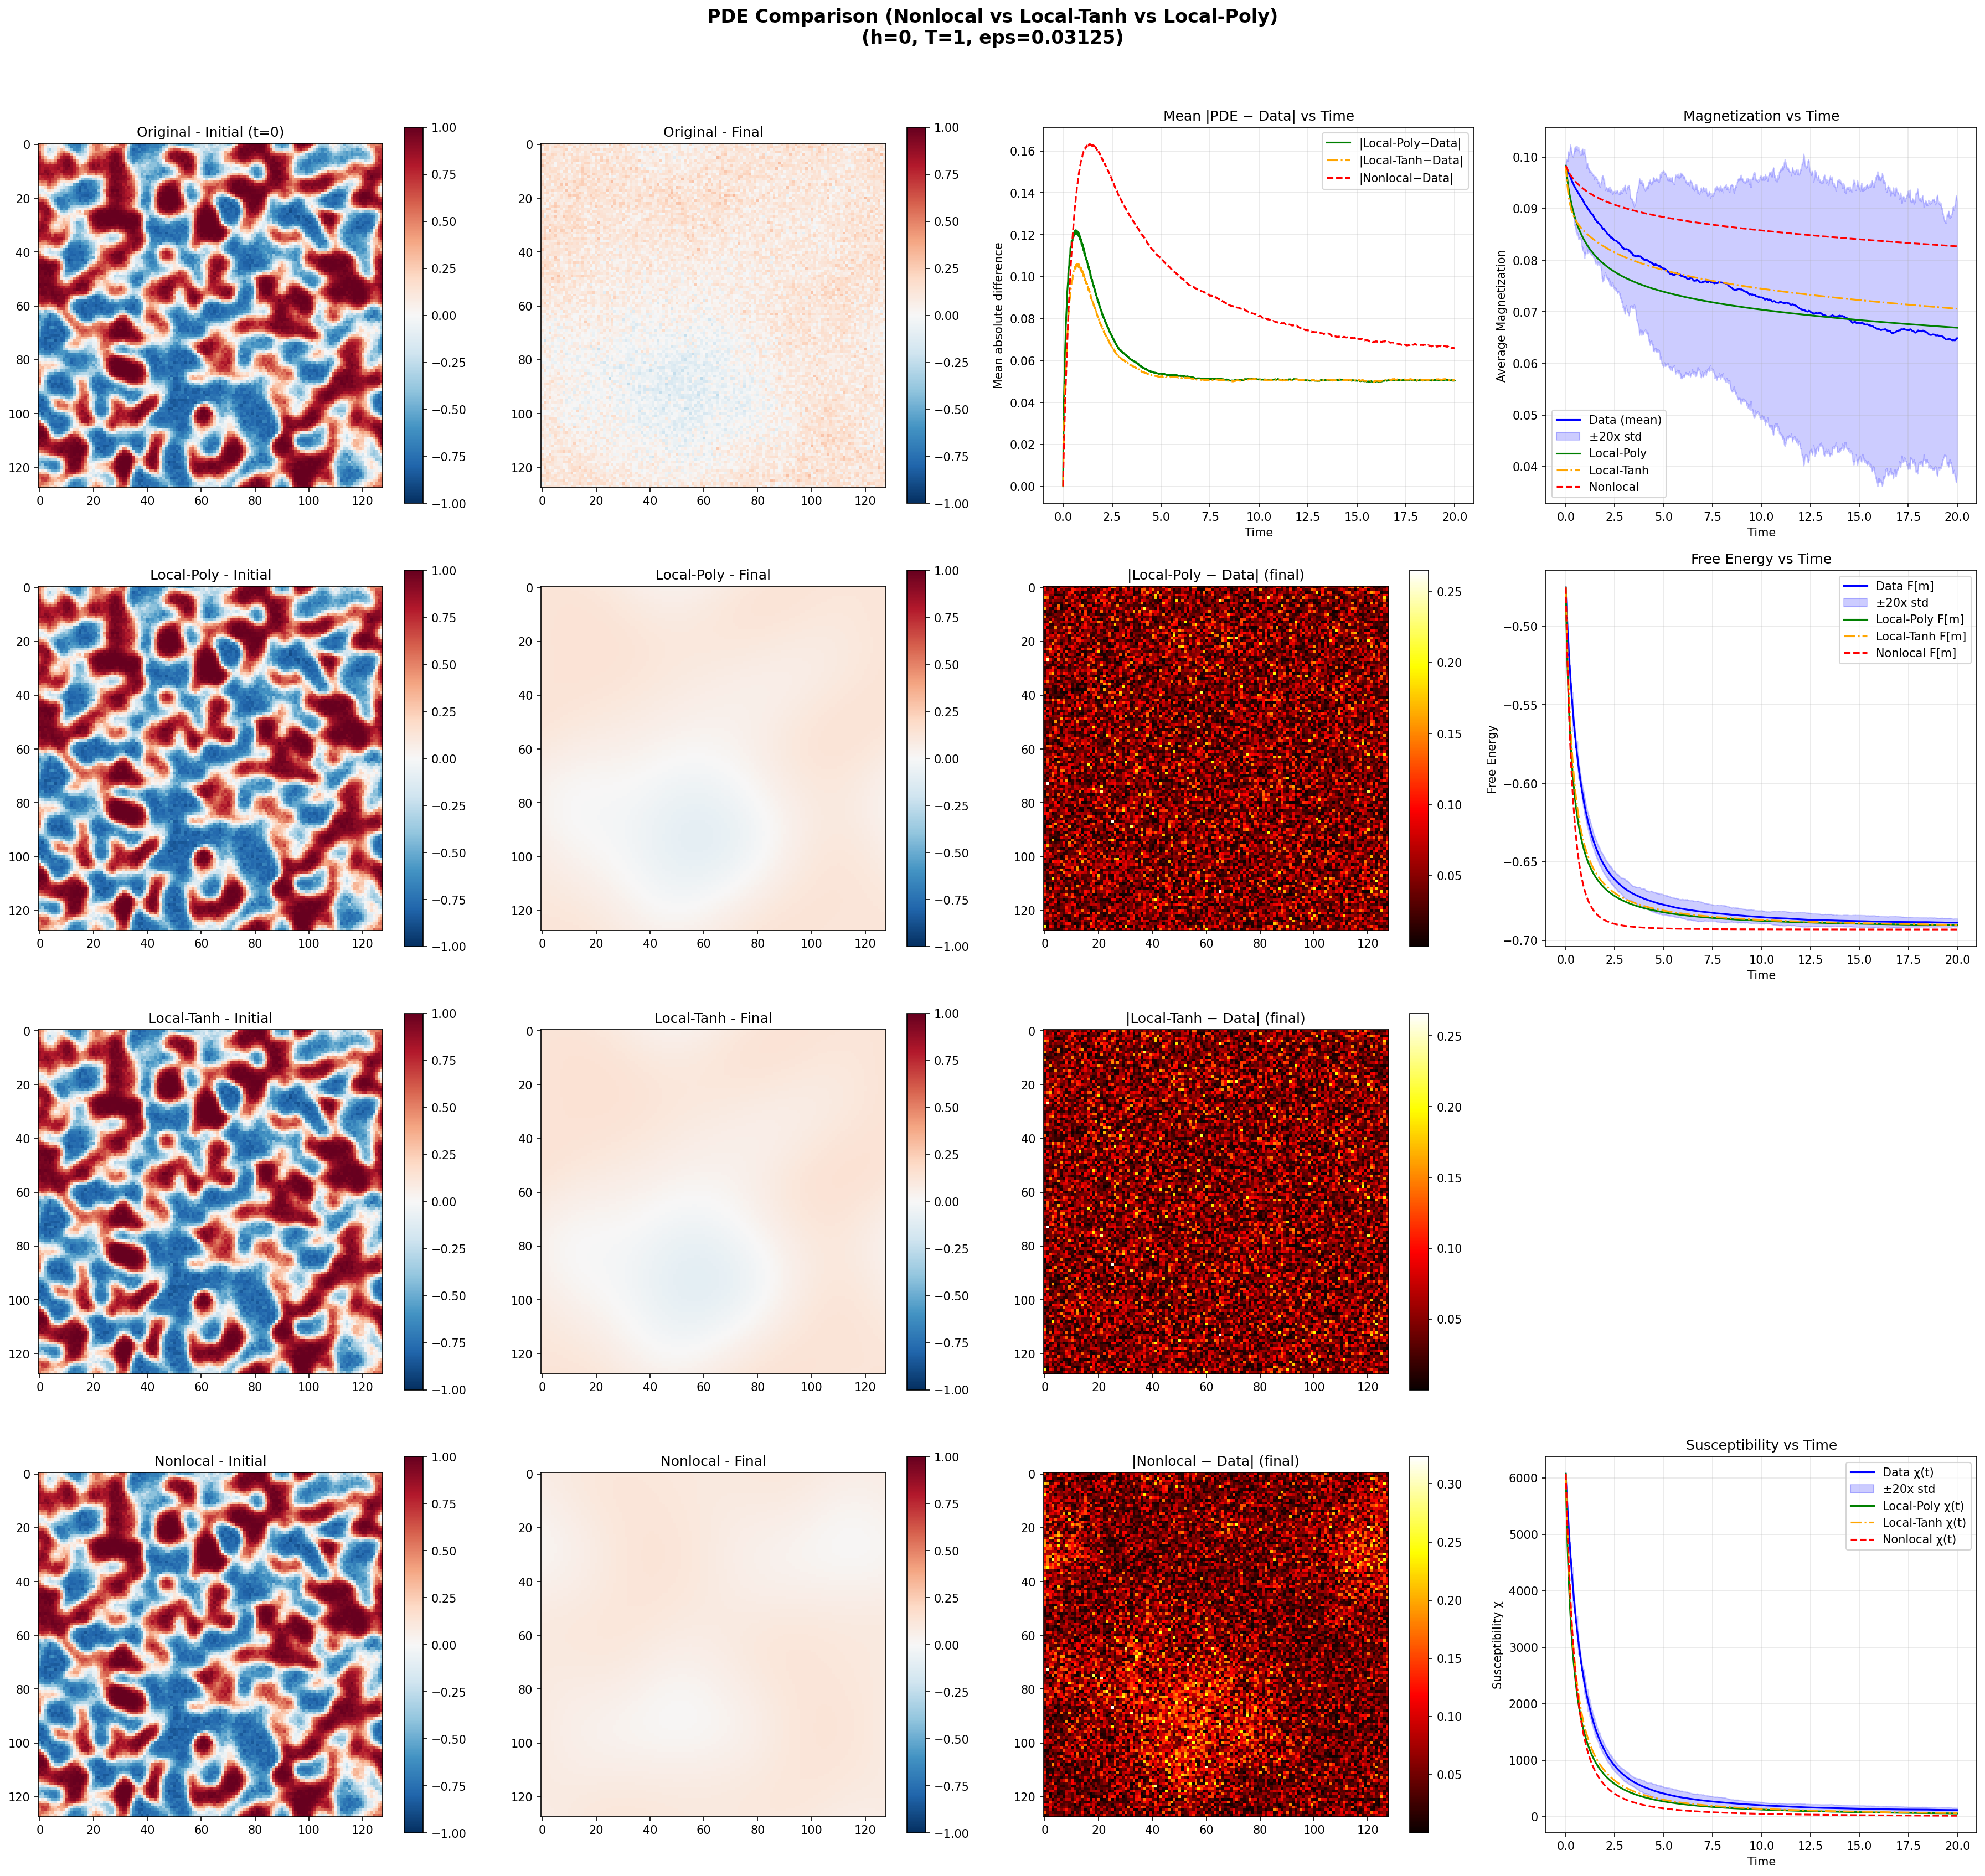
\includegraphics[width=1.0\textwidth]{fig/compare_pde_solvers_L2048_h0_T1_eps0.03125.png}
% 	\caption{Comparison of original data and PDE solutions for $h=0$, $T=1$, $\epsilon=0.03125$, $L=2048$.}
% 	\label{fig:pde_comparison_h0_T1_eps0.03125_L2048}
% \end{figure}


% \begin{figure}[h]
% 	\centering
% 	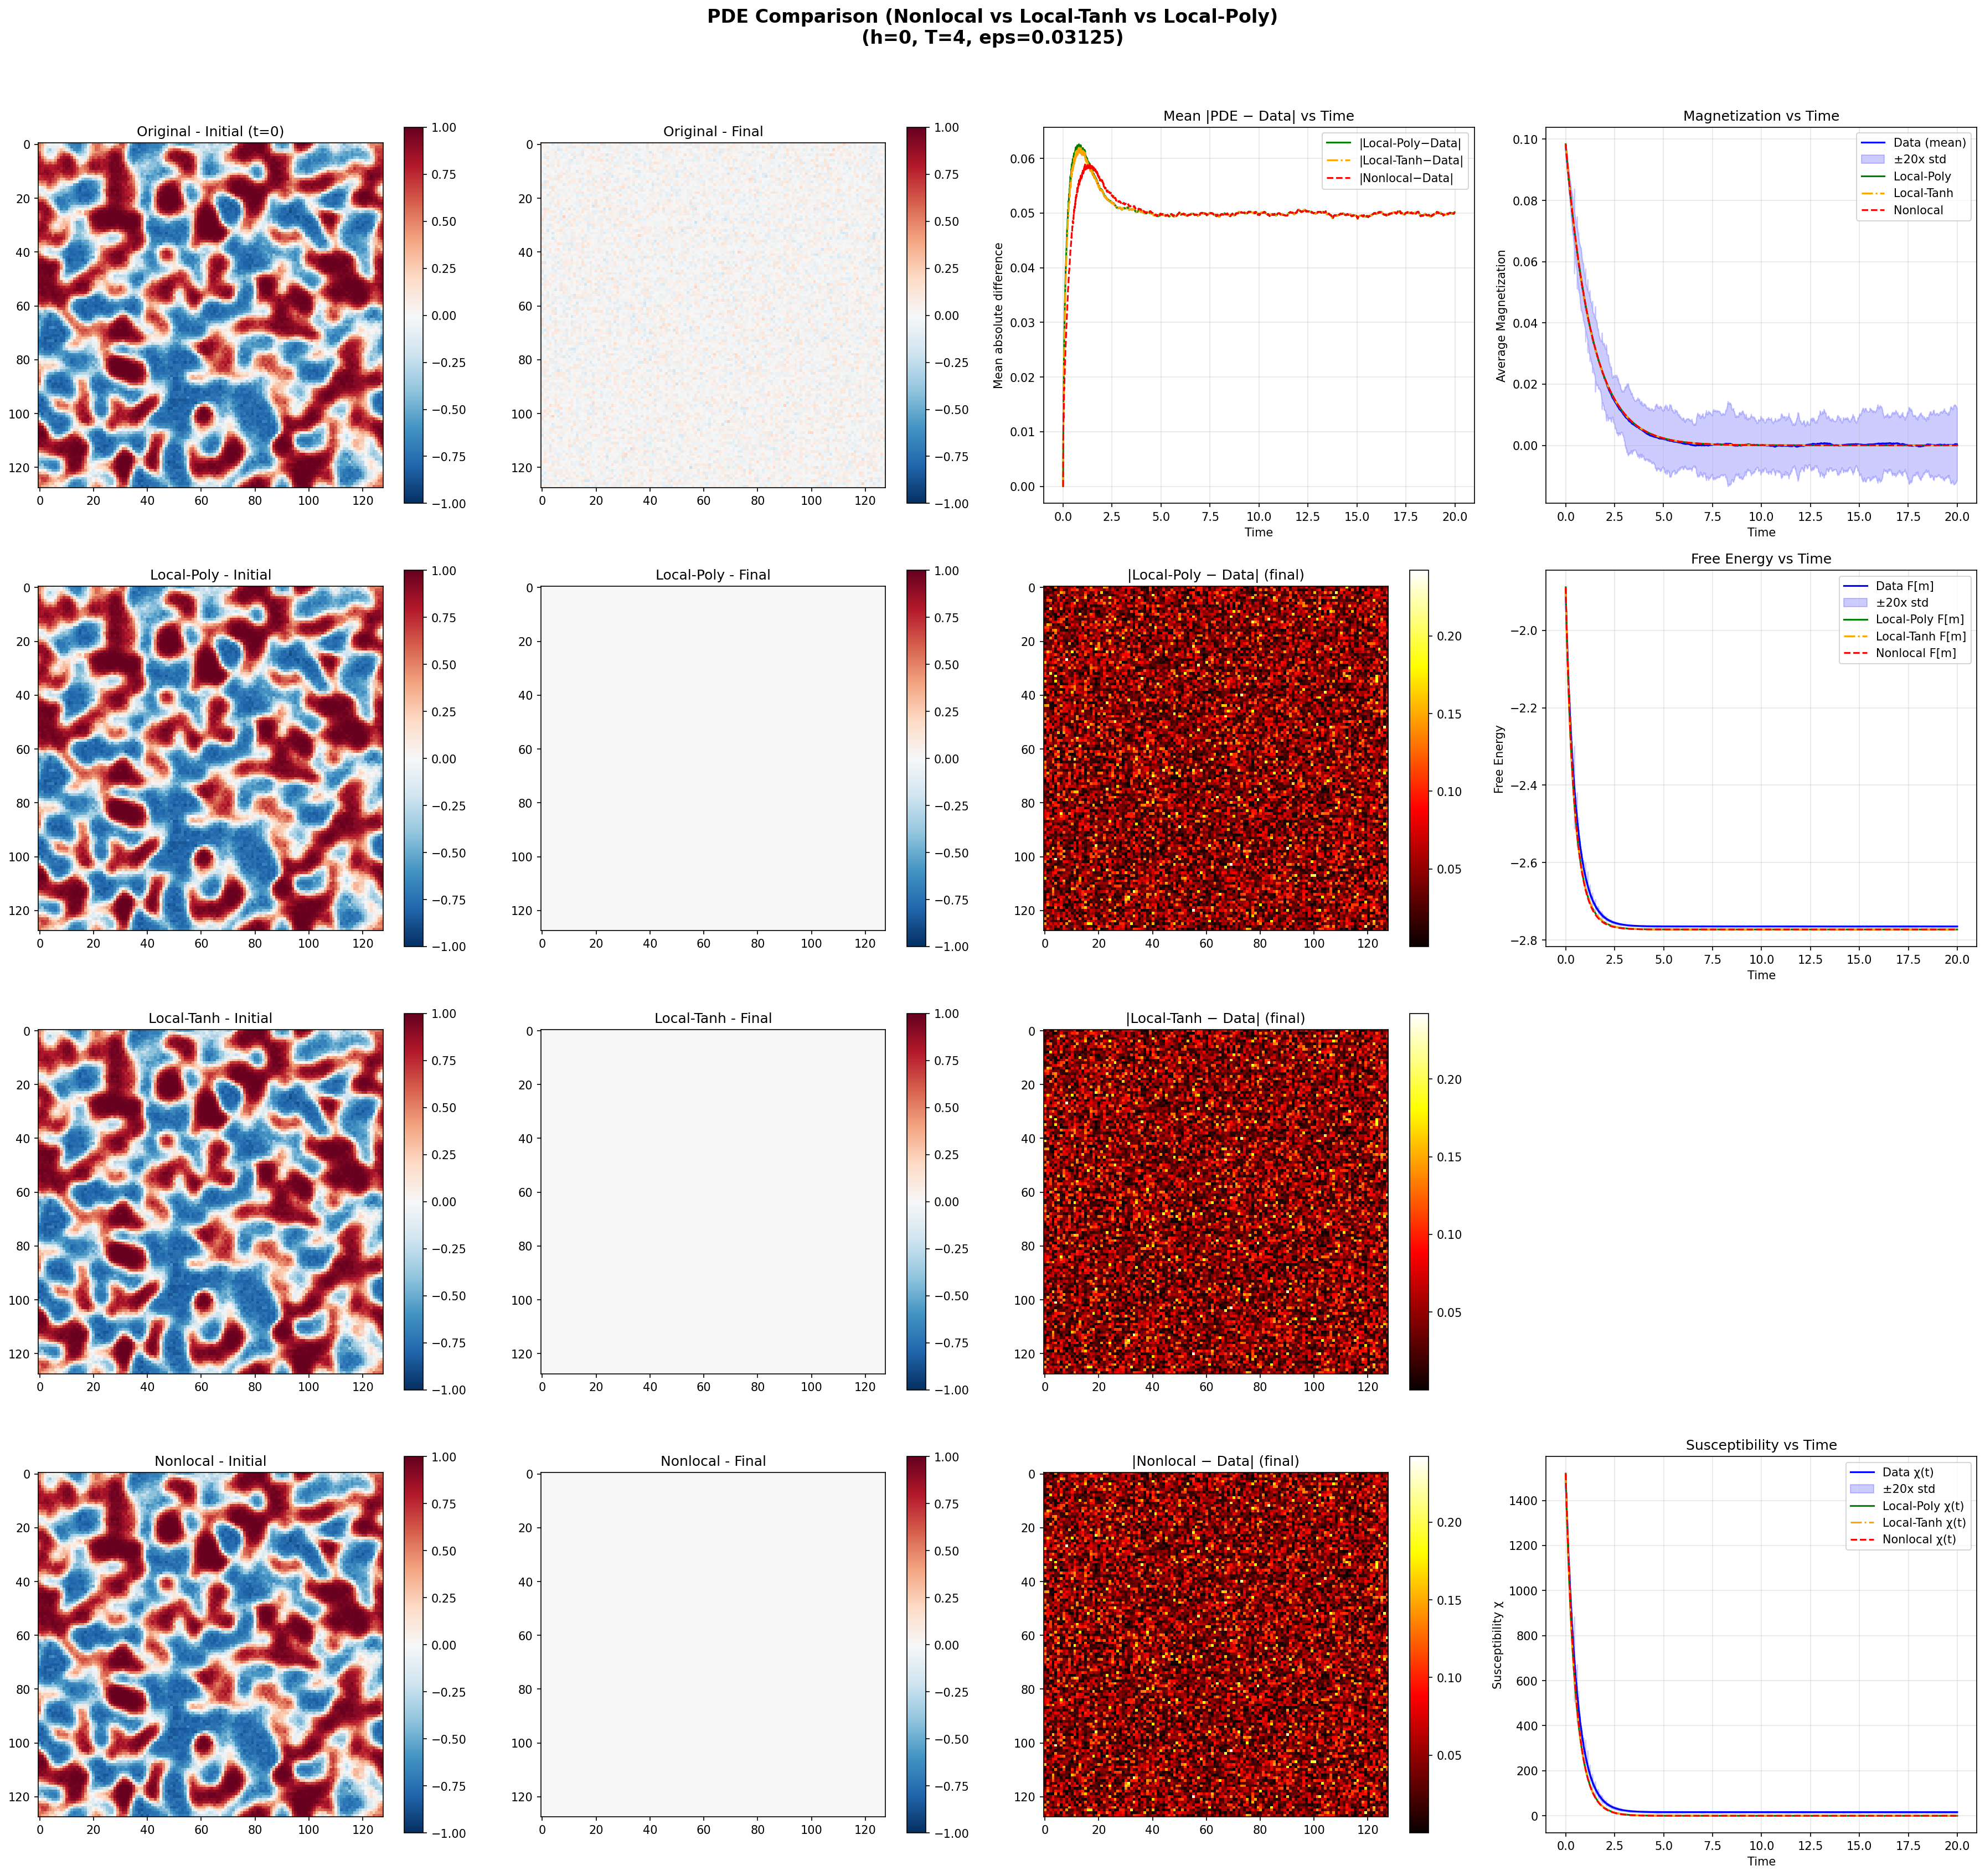
\includegraphics[width=1.0\textwidth]{fig/compare_pde_solvers_L2048_h0_T4_eps0.03125.png}
% 	\caption{Comparison of original data and PDE solutions for $h=0$, $T=4$, $\epsilon=0.03125$, $L=2048$.}
% 	\label{fig:pde_comparison_h0_T4_eps0.03125_L2048}
% \end{figure}


% \begin{figure}[!h]
% 	\centering
% 	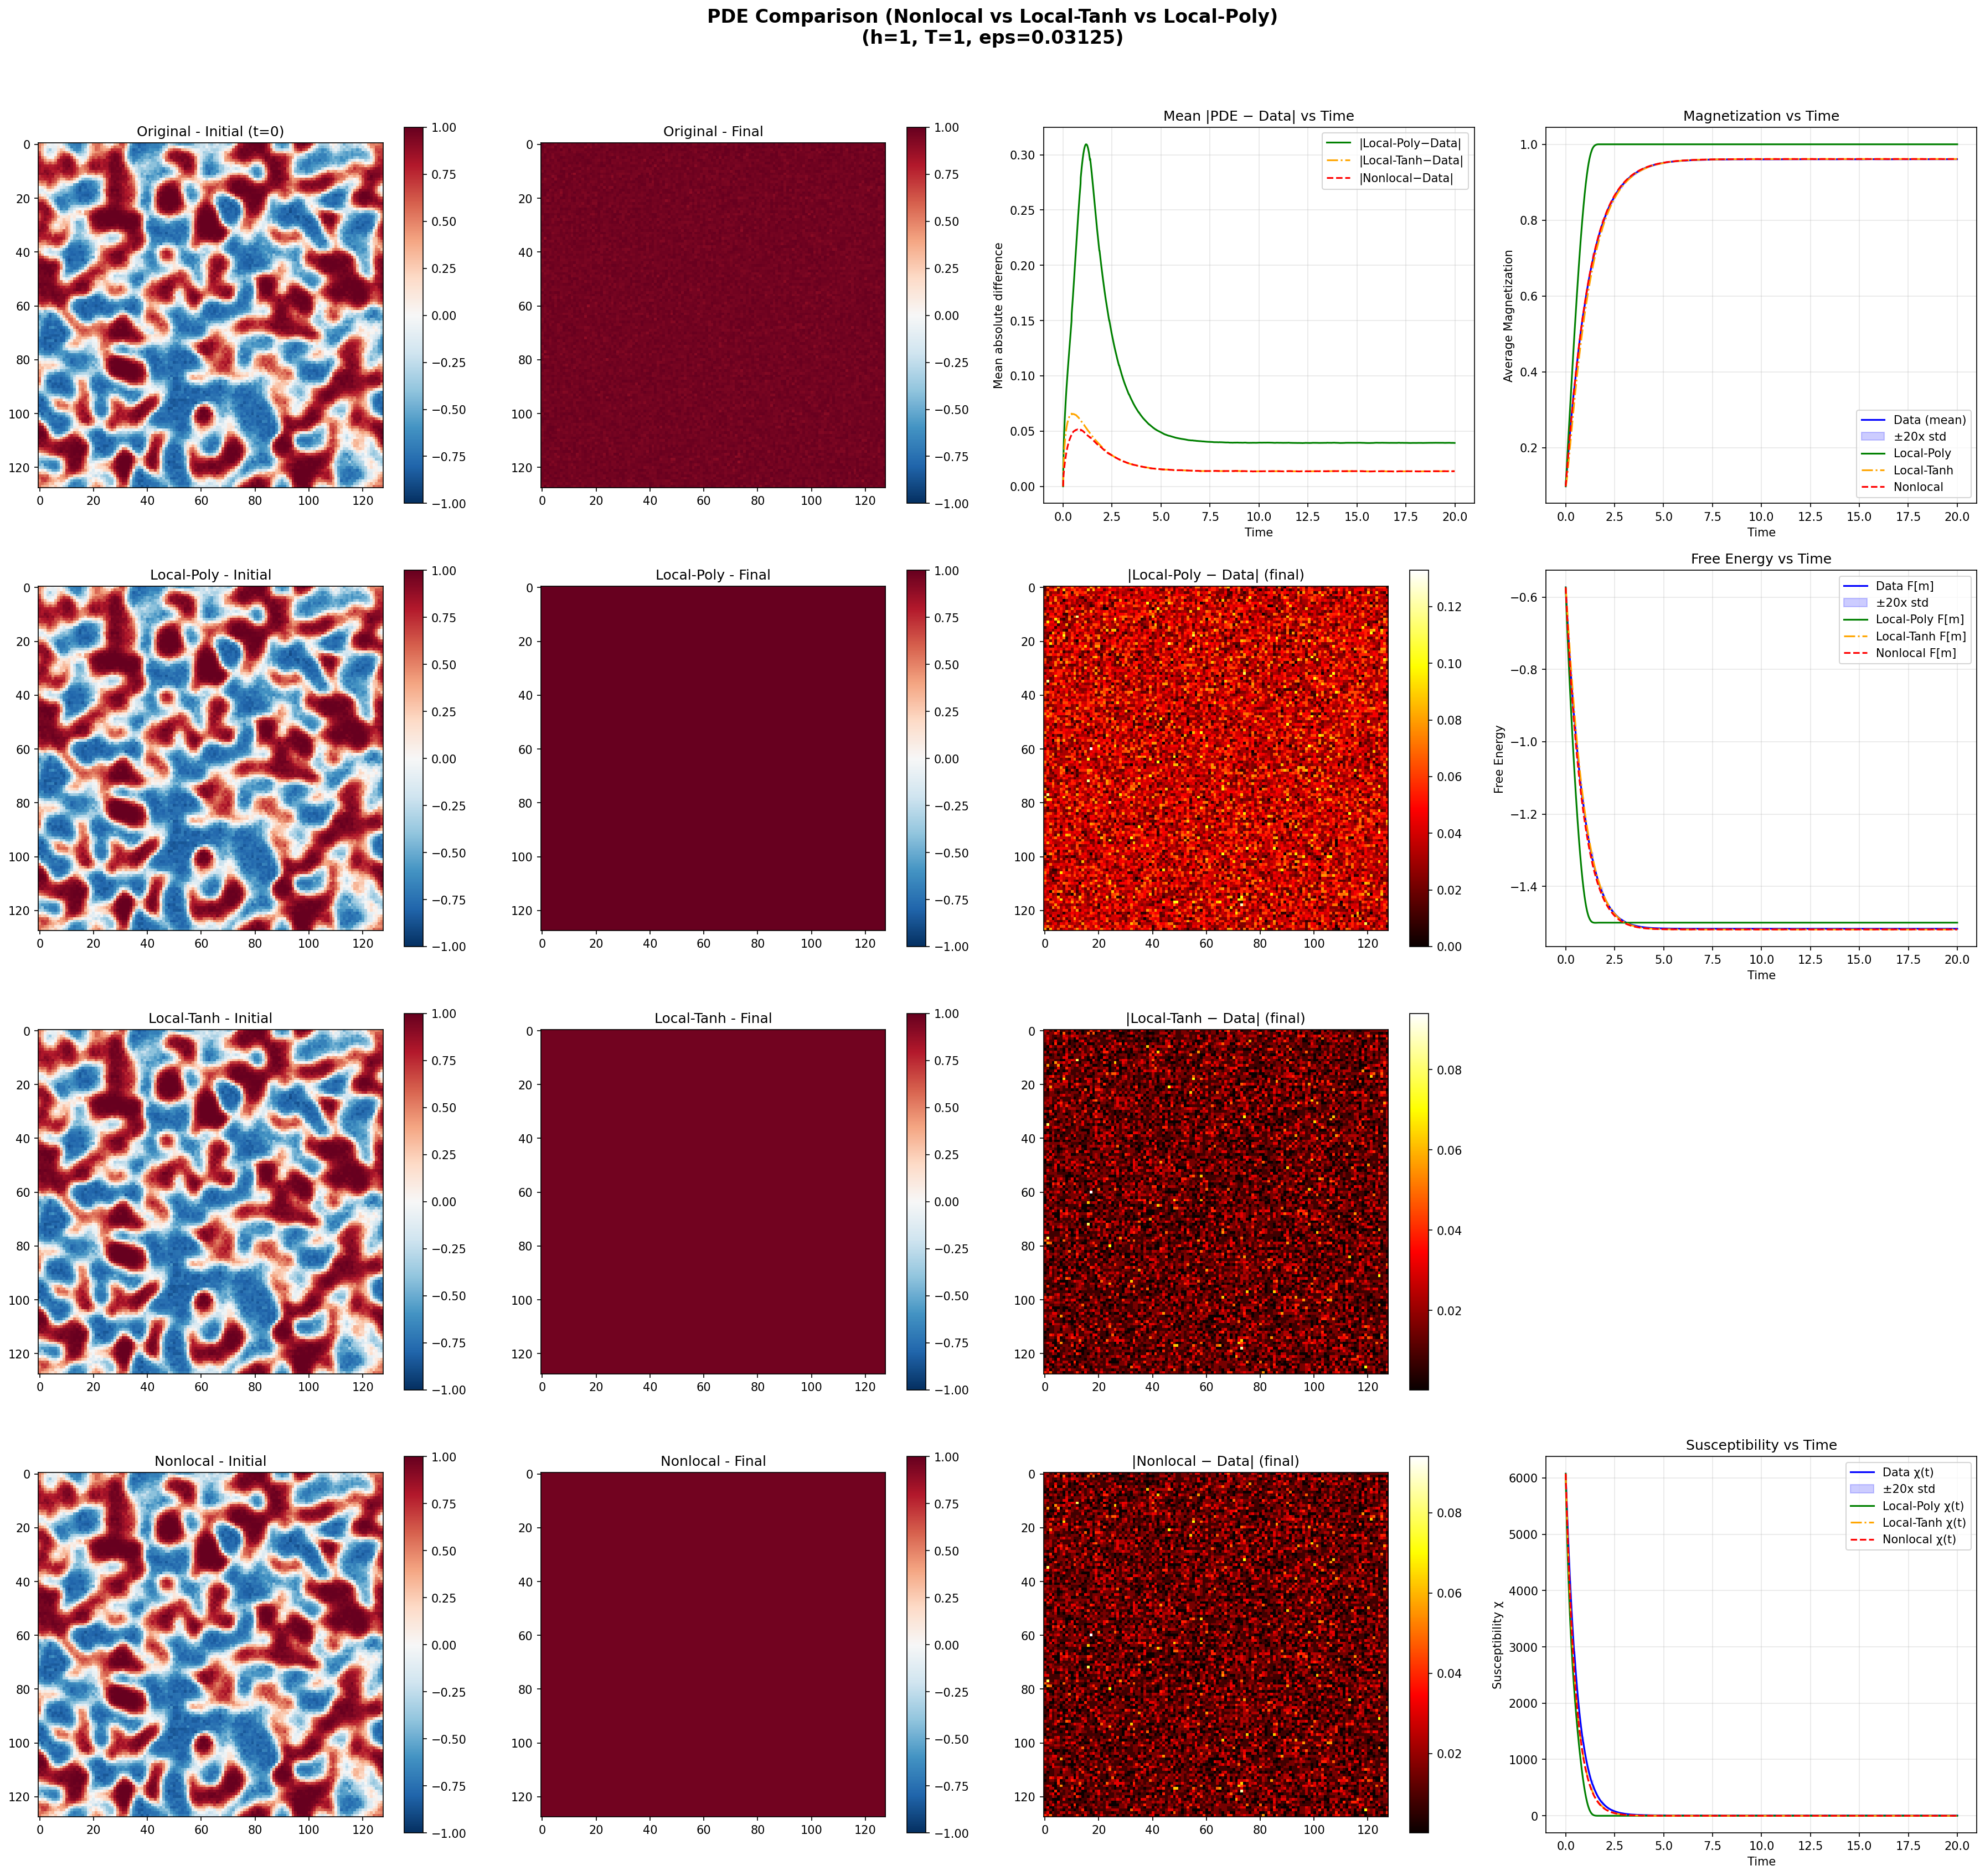
\includegraphics[width=1.0\textwidth]{fig/compare_pde_solvers_L2048_h1_T1_eps0.03125.png}
% 	\caption{Comparison of original data and PDE solutions for $h=1$, $T=1$, $\epsilon=0.03125$, $L=2048$.}
% 	\label{fig:pde_comparison_h1_T1_eps0.03125_L2048}
% \end{figure}


% \begin{figure}[h]
% 	\centering
% 	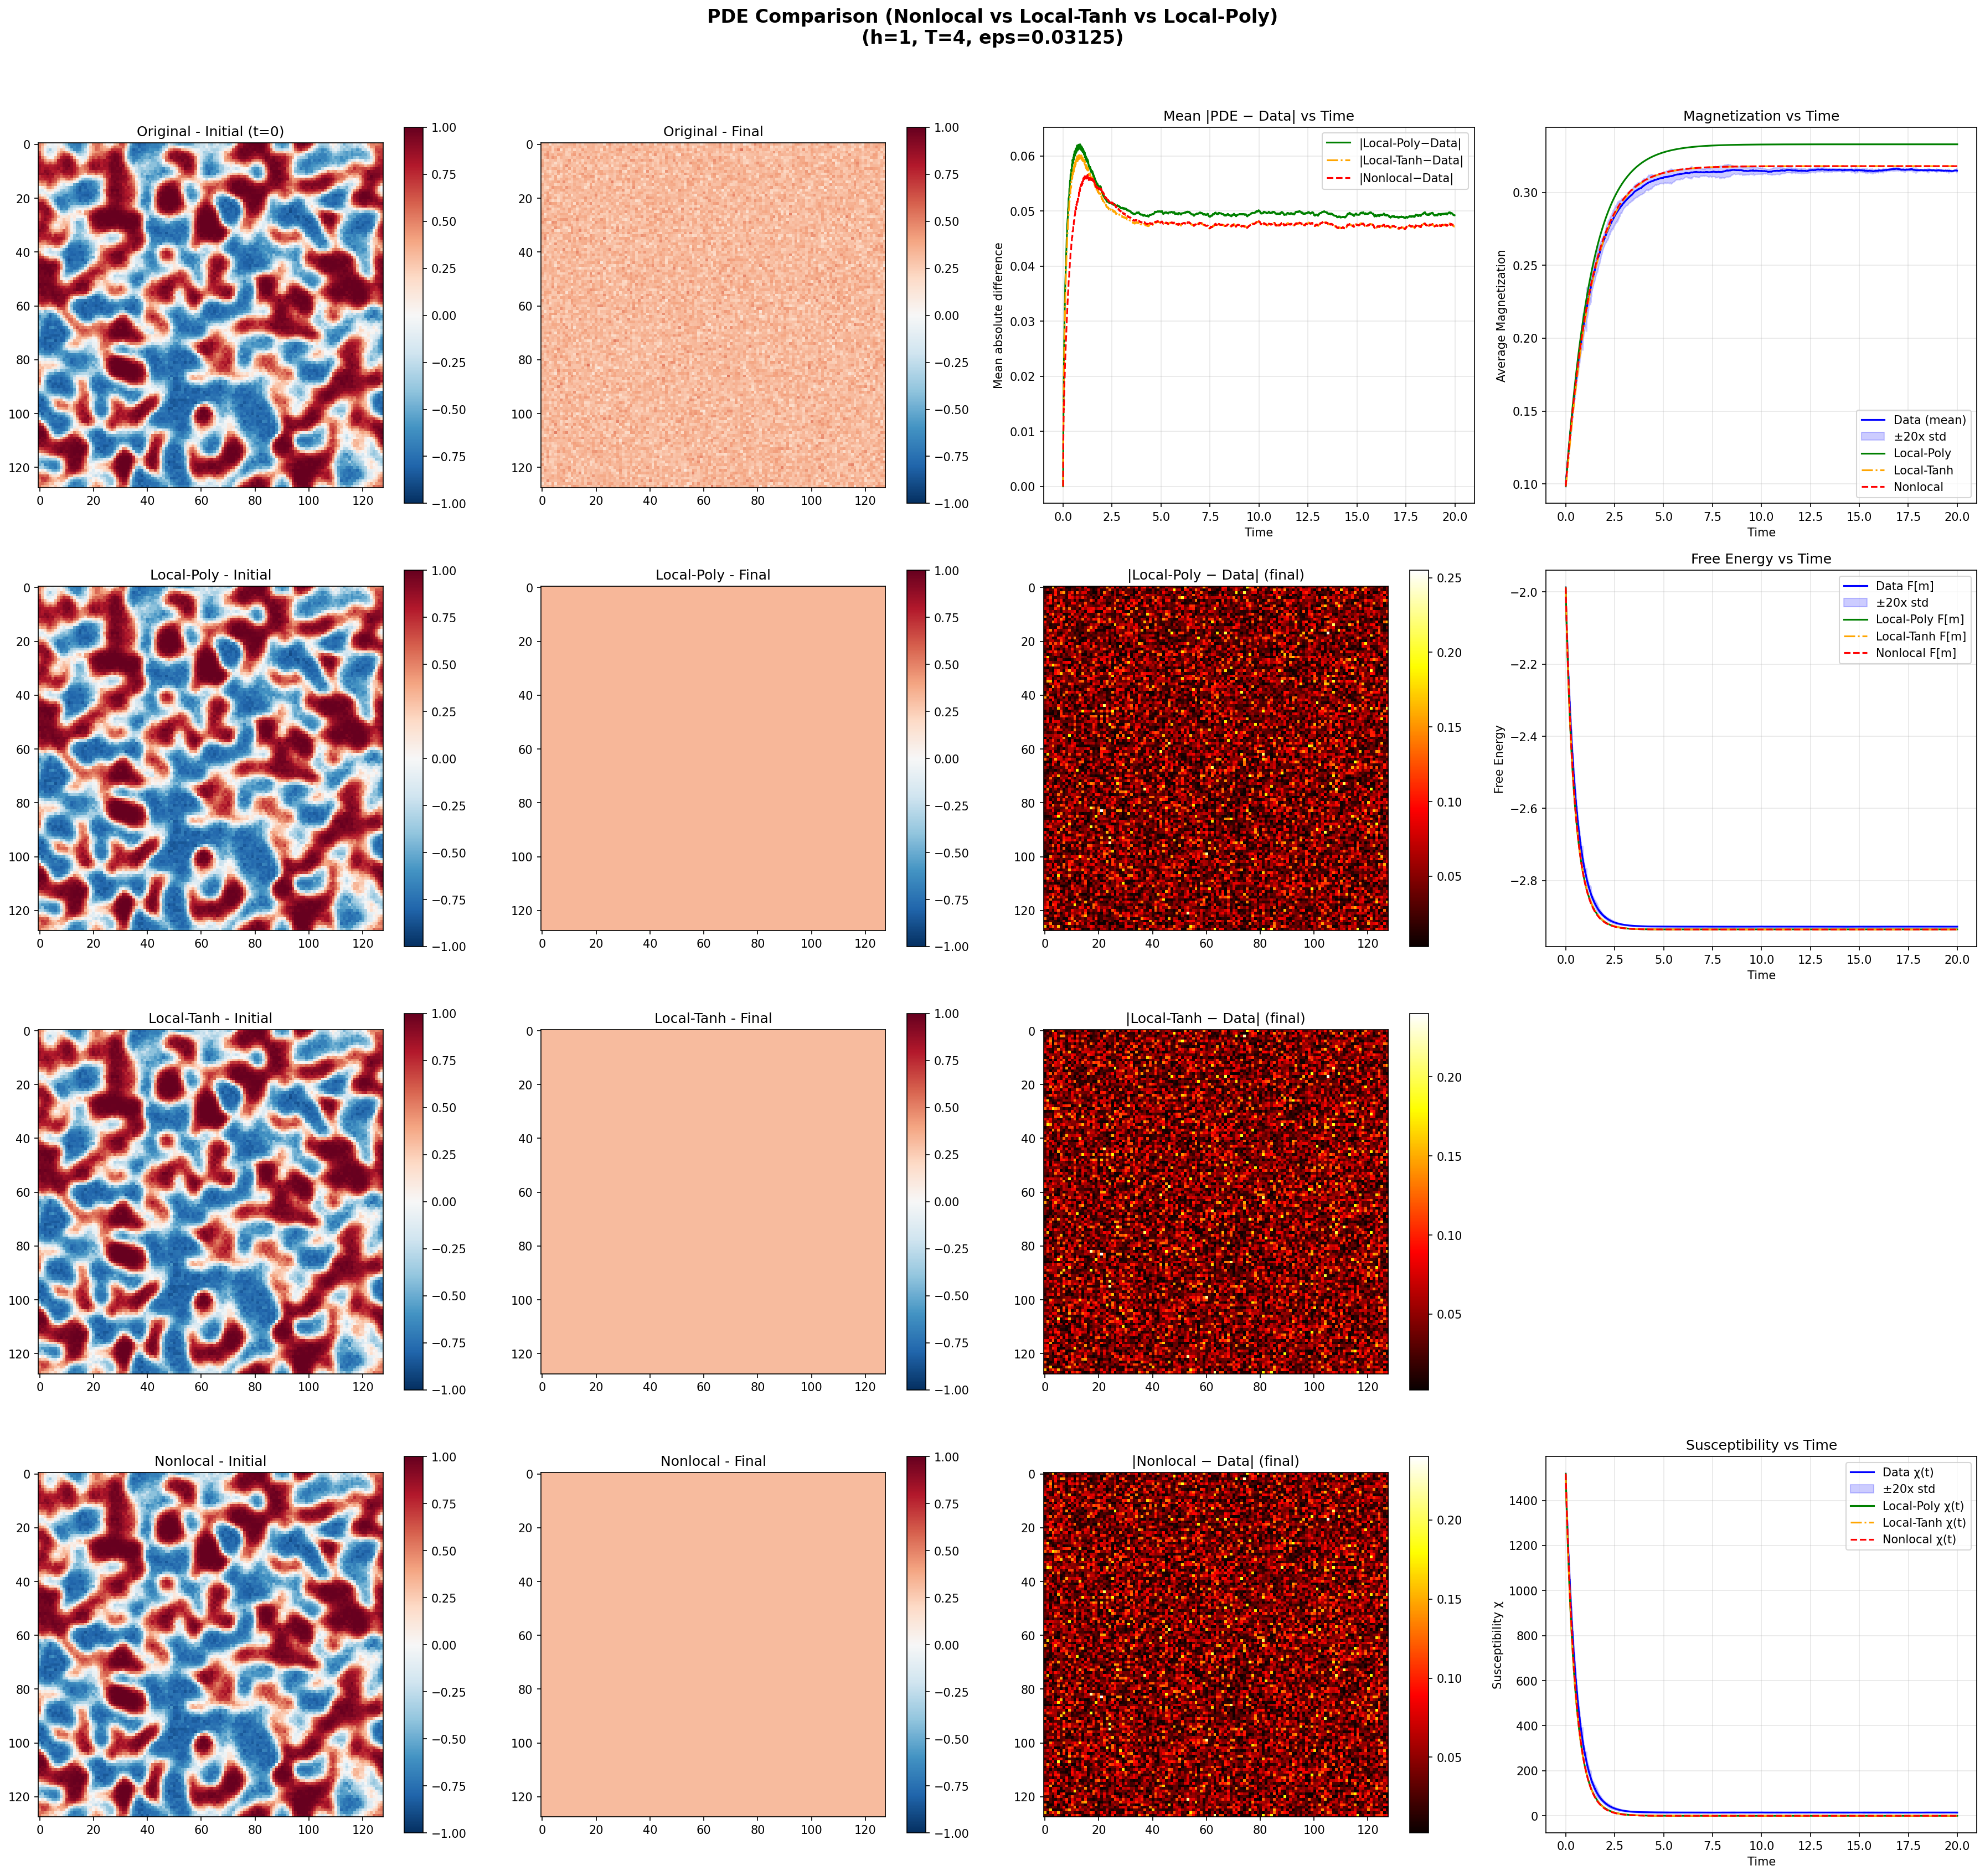
\includegraphics[width=1.0\textwidth]{fig/compare_pde_solvers_L2048_h1_T4_eps0.03125.png}
% 	\caption{Comparison of original data and PDE solutions for $h=1$, $T=4$, $\epsilon=0.03125$, $L=2048$.}
% 	\label{fig:pde_comparison_h1_T4_eps0.03125_L2048}
% \end{figure}


% % with epsilon = 0.0625, L = 2048

% \begin{figure}[!h]
% 	\centering
% 	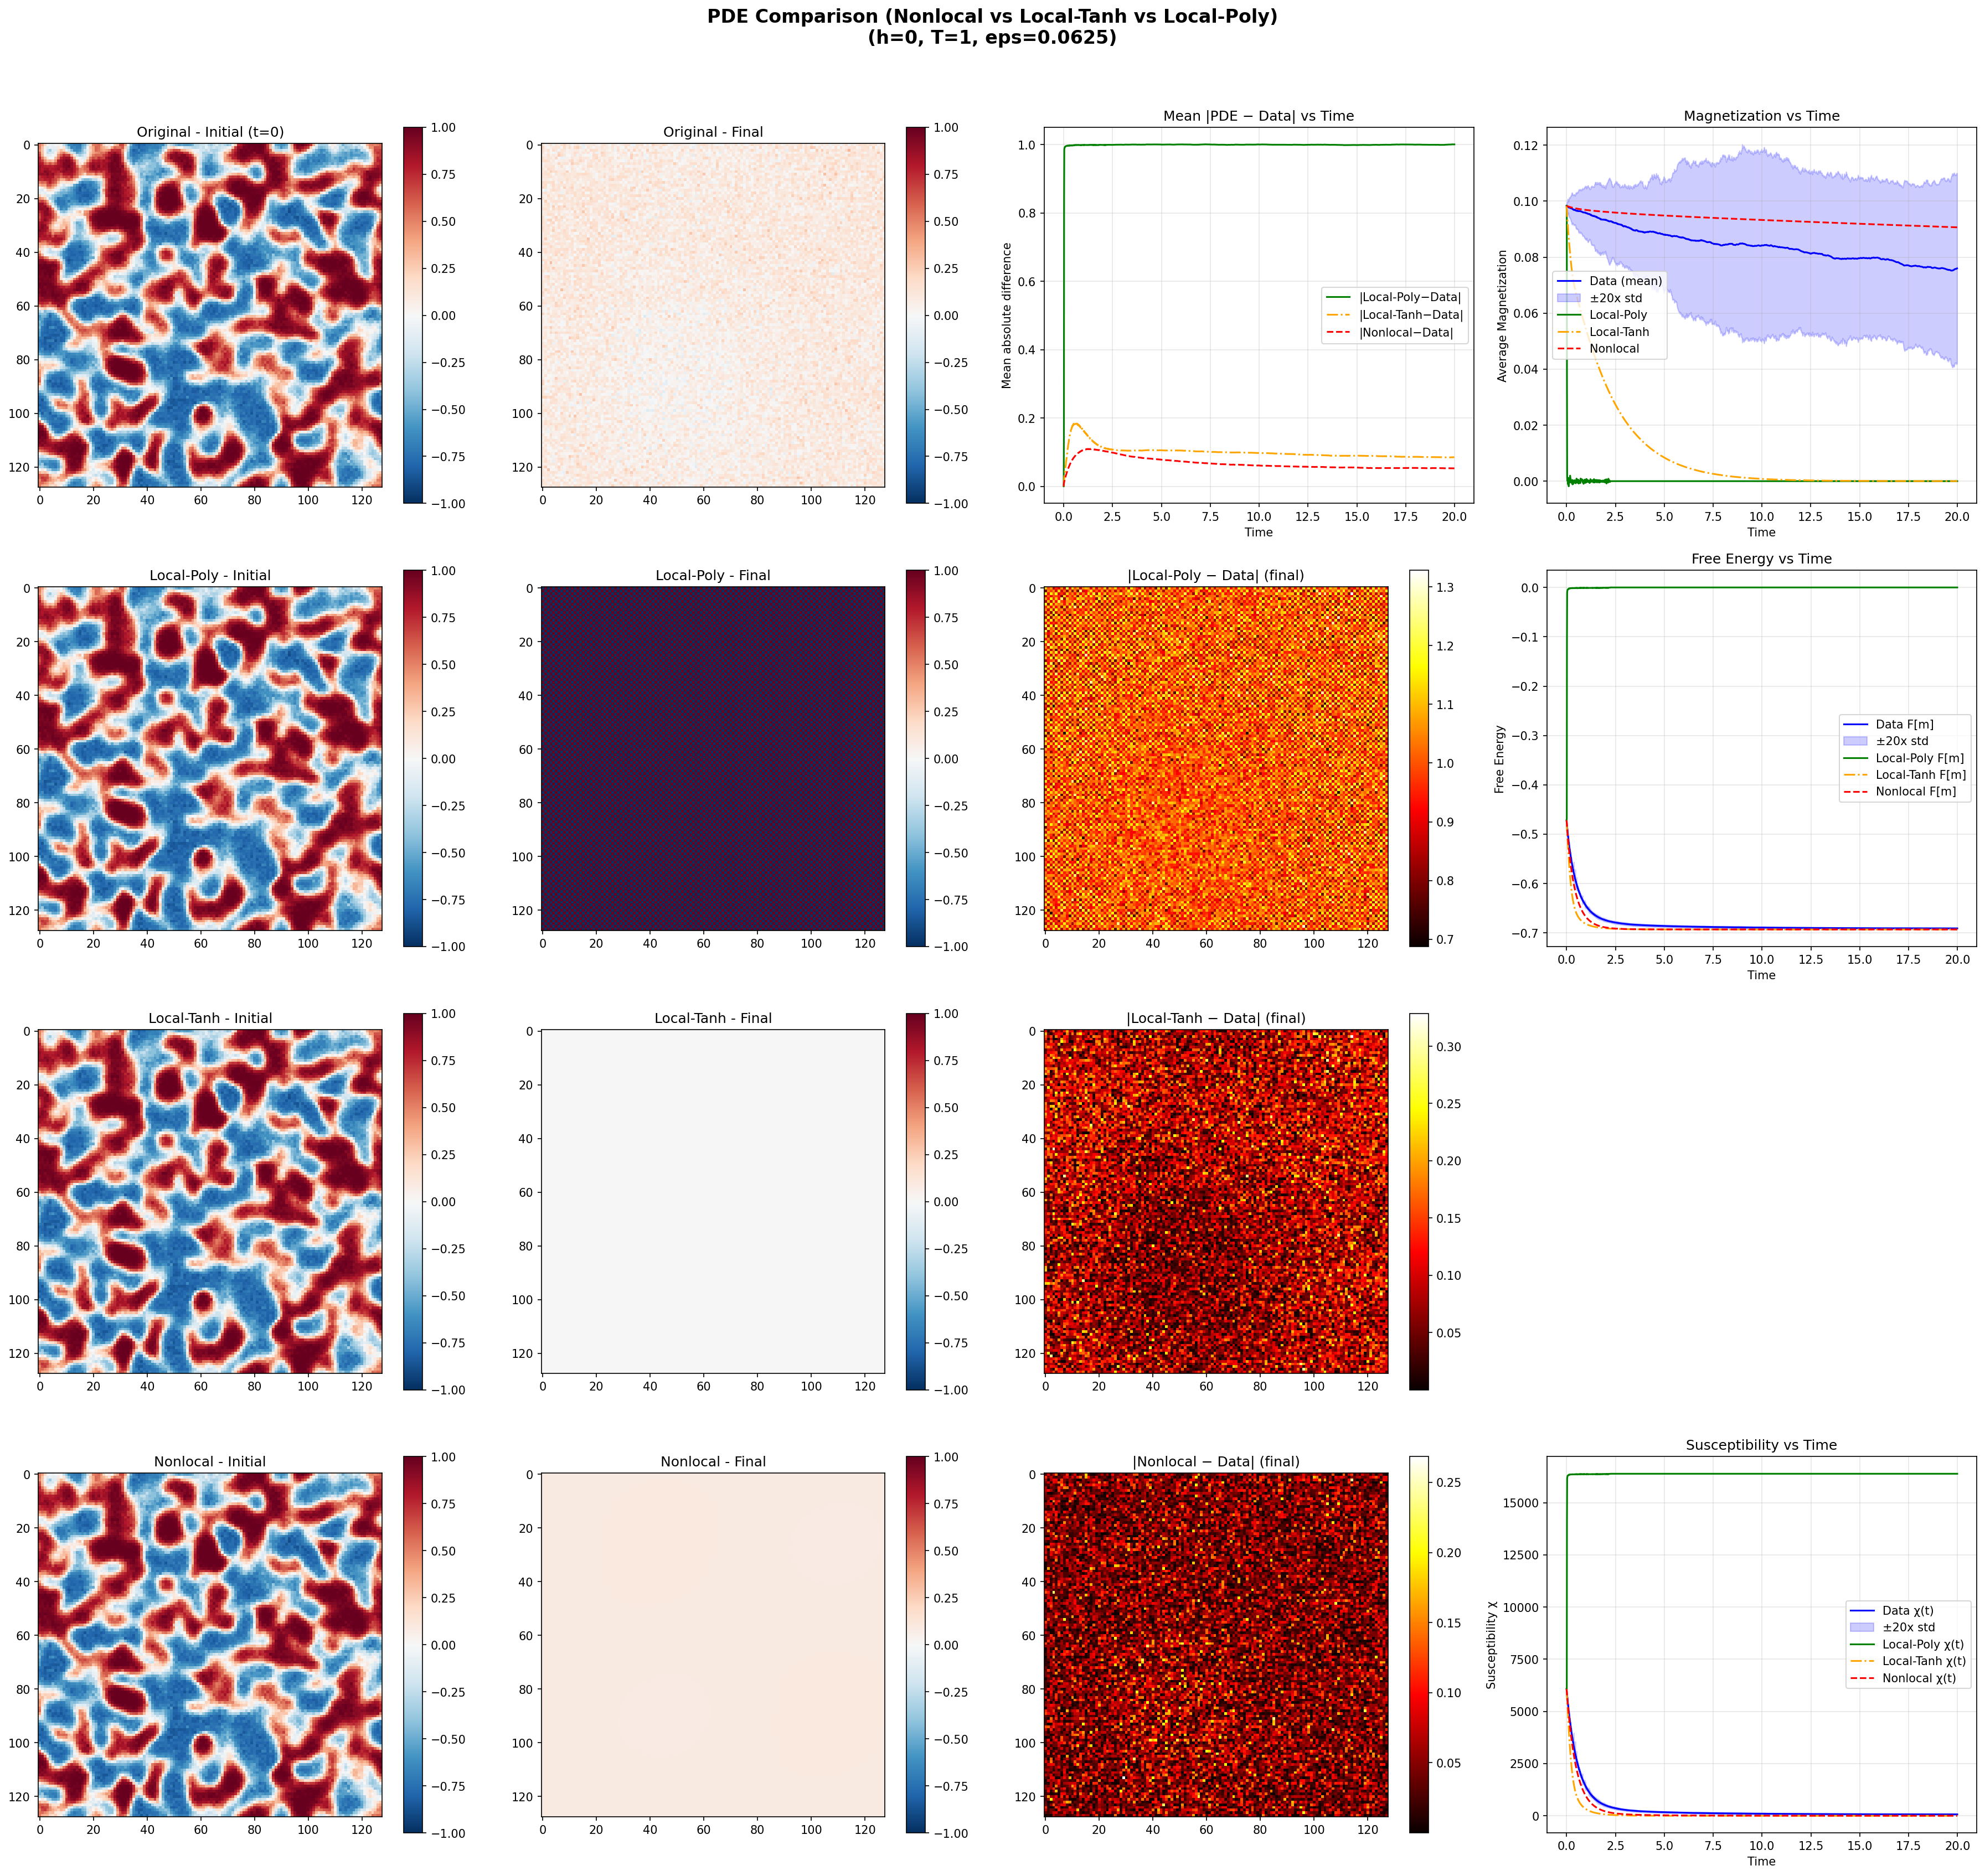
\includegraphics[width=1.0\textwidth]{fig/compare_pde_solvers_L2048_h0_T1_eps0.0625.png}
% 	\caption{Comparison of original data and PDE solutions for $h=0$, $T=1$, $\epsilon=0.0625$, $L=2048$.}
% 	\label{fig:pde_comparison_h0_T1_eps0.0625_L2048}
% \end{figure}


% \begin{figure}[!h]
% 	\centering
% 	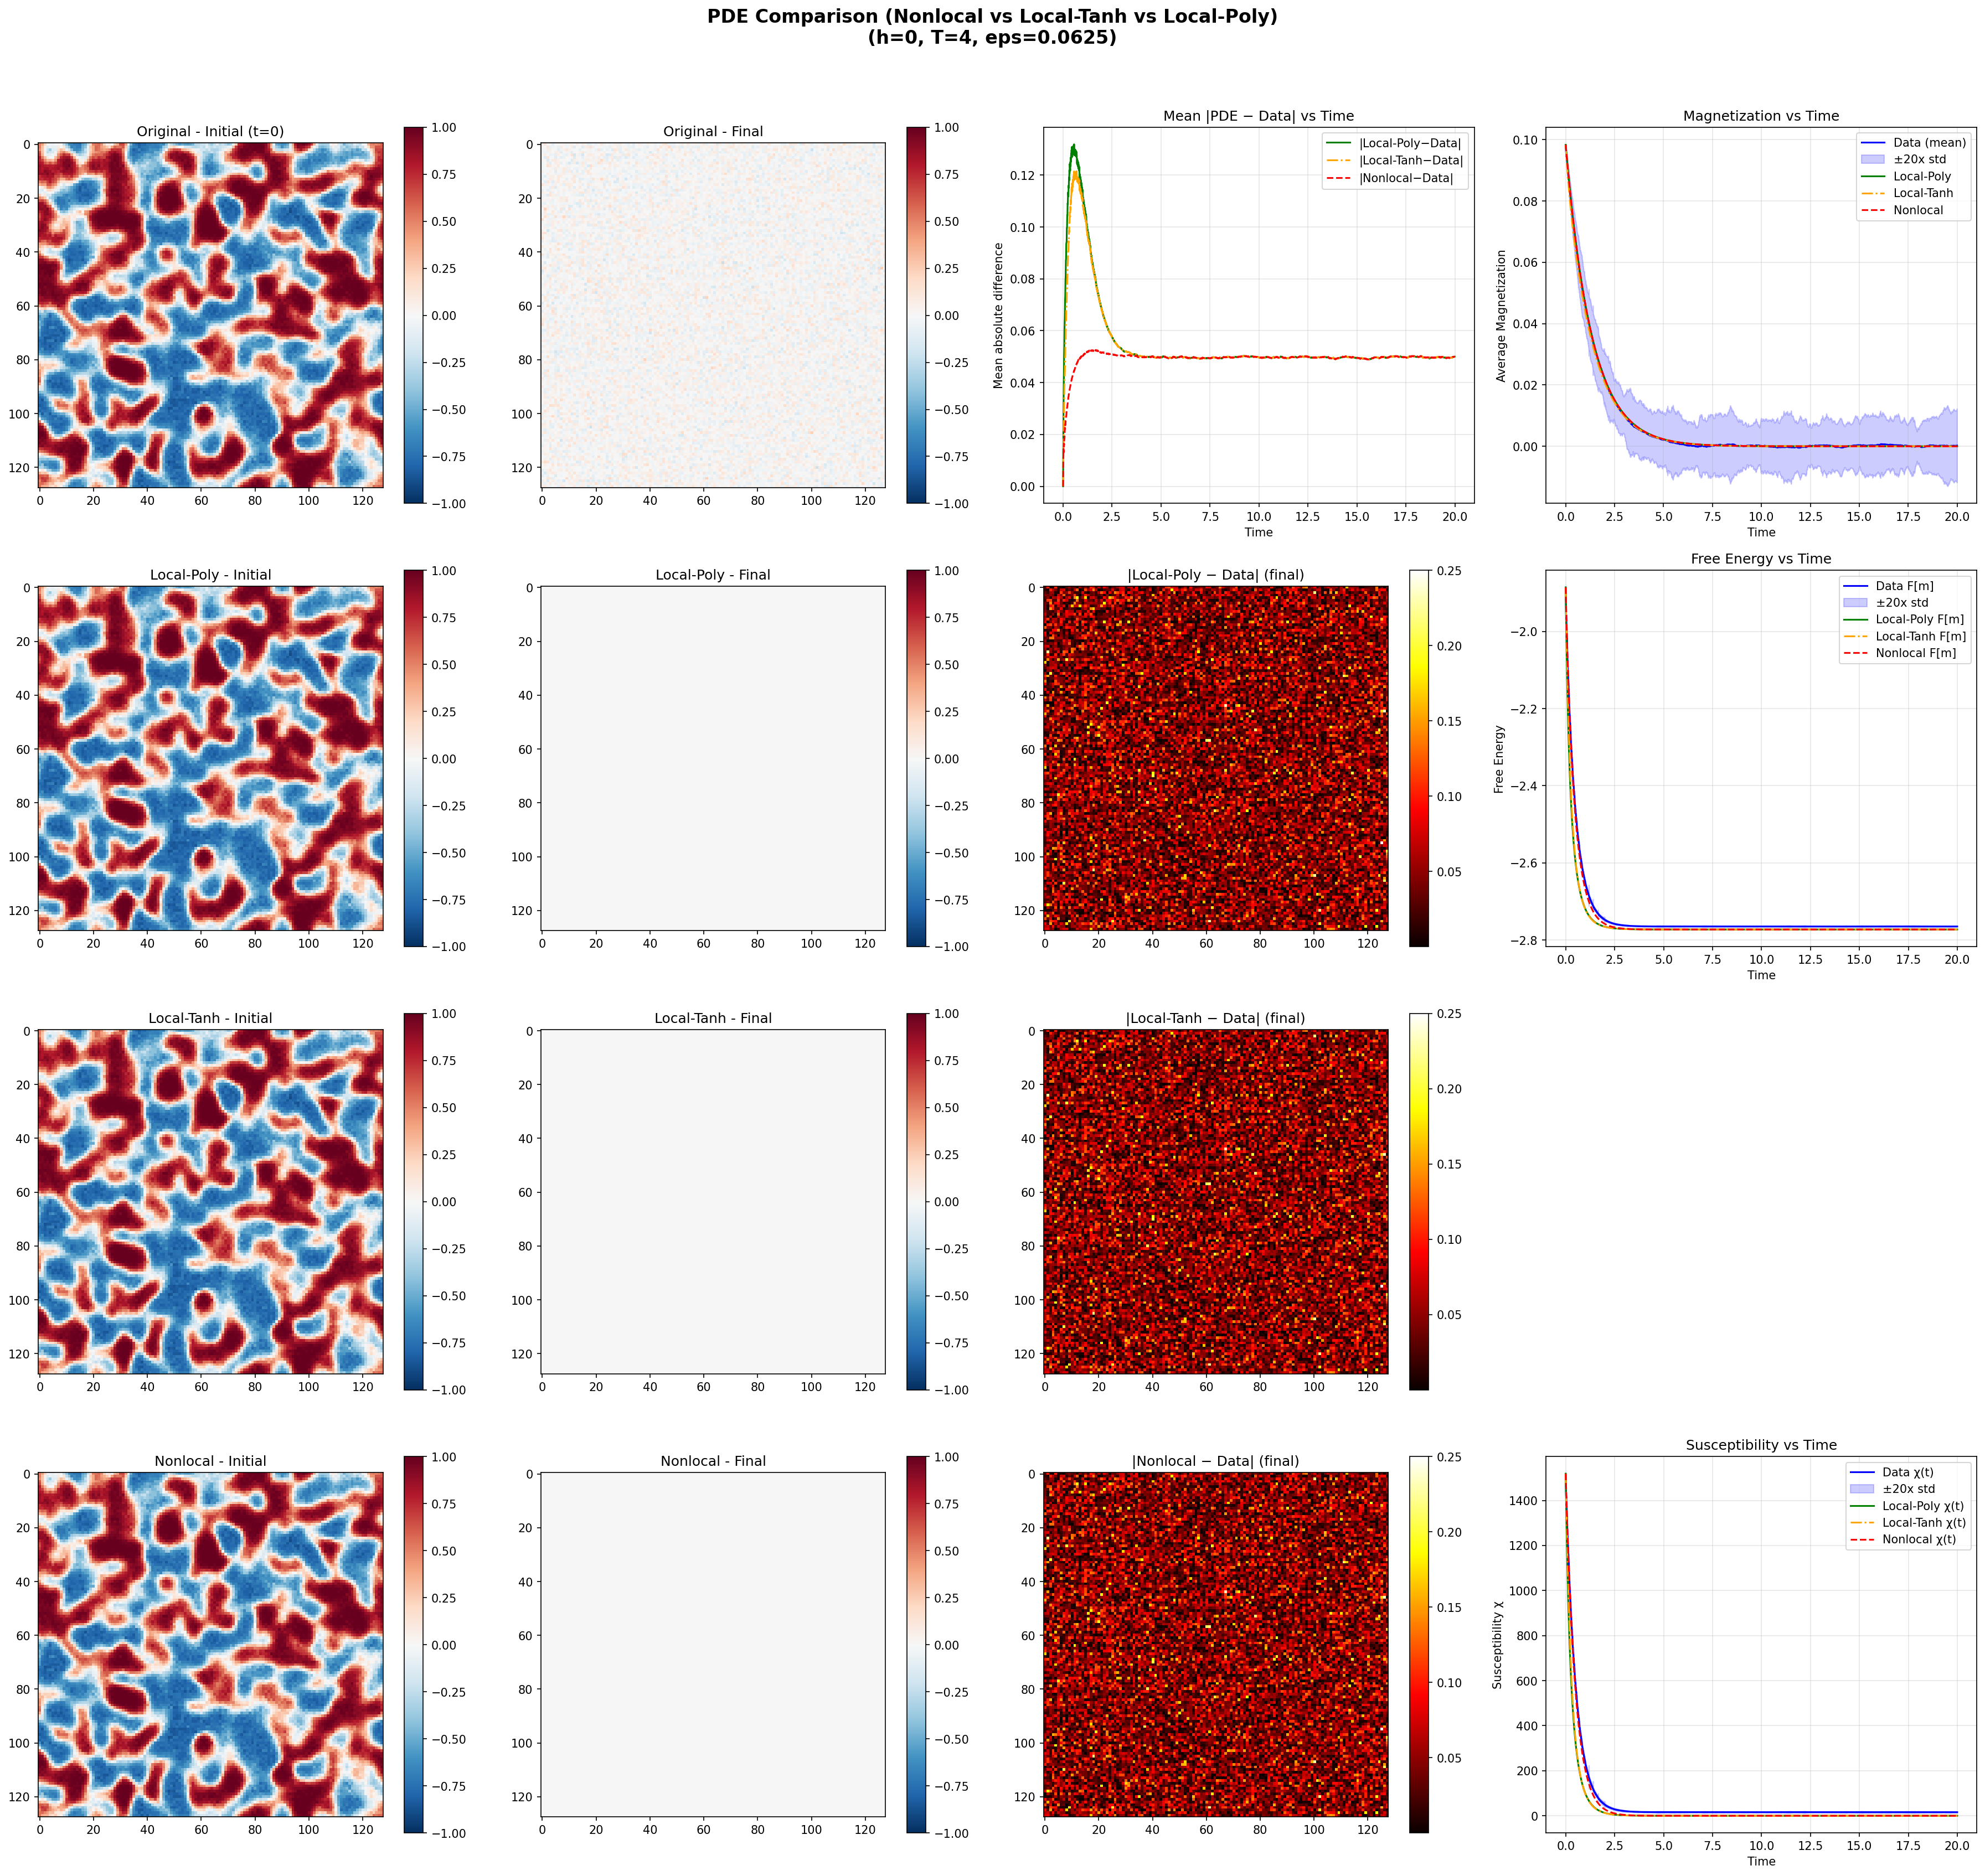
\includegraphics[width=1.0\textwidth]{fig/compare_pde_solvers_L2048_h0_T4_eps0.0625.png}
% 	\caption{Comparison of original data and PDE solutions for $h=0$, $T=4$, $\epsilon=0.0625$, $L=2048$.}
% 	\label{fig:pde_comparison_h0_T4_eps0.0625_L2048}
% \end{figure}

% \begin{figure}[!h]
% 	\centering
% 	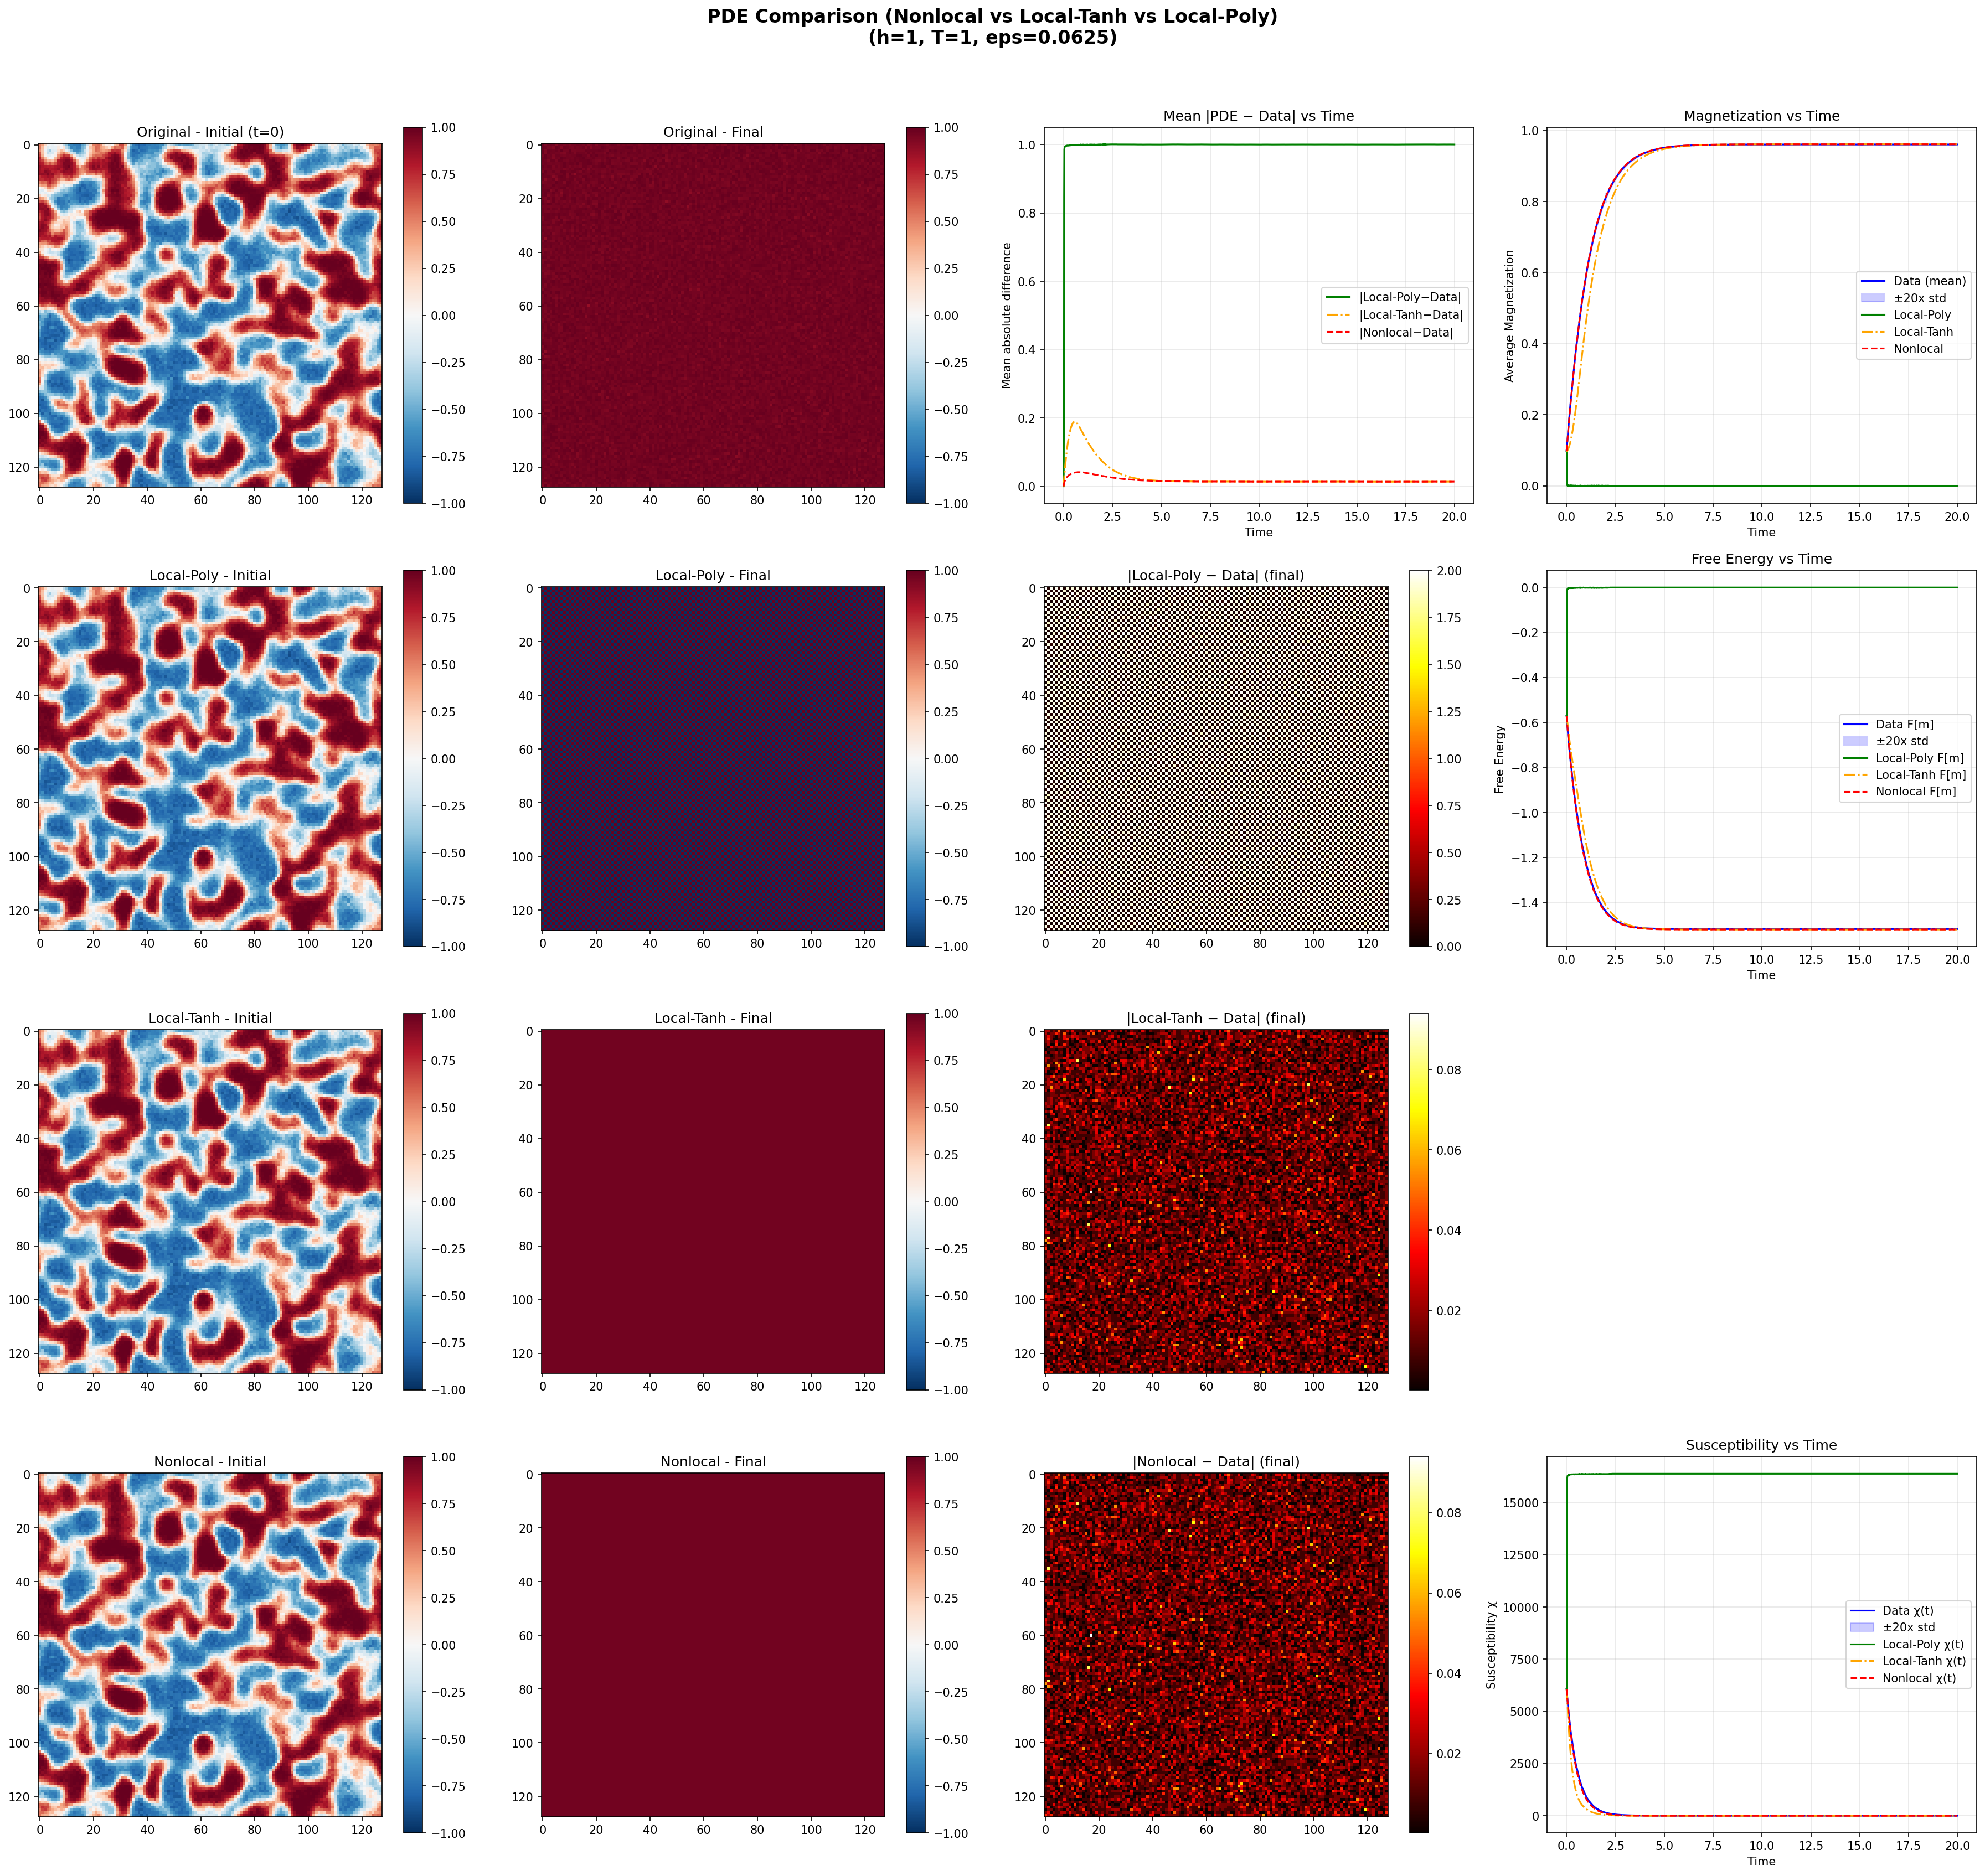
\includegraphics[width=1.0\textwidth]{fig/compare_pde_solvers_L2048_h1_T1_eps0.0625.png}
% 	\caption{Comparison of original data and PDE solutions for $h=1$, $T=1$, $\epsilon=0.0625$, $L=2048$.}
% 	\label{fig:pde_comparison_h1_T1_eps0.0625_L2048}
% \end{figure}

% \begin{figure}[!h]
% 	\centering
% 	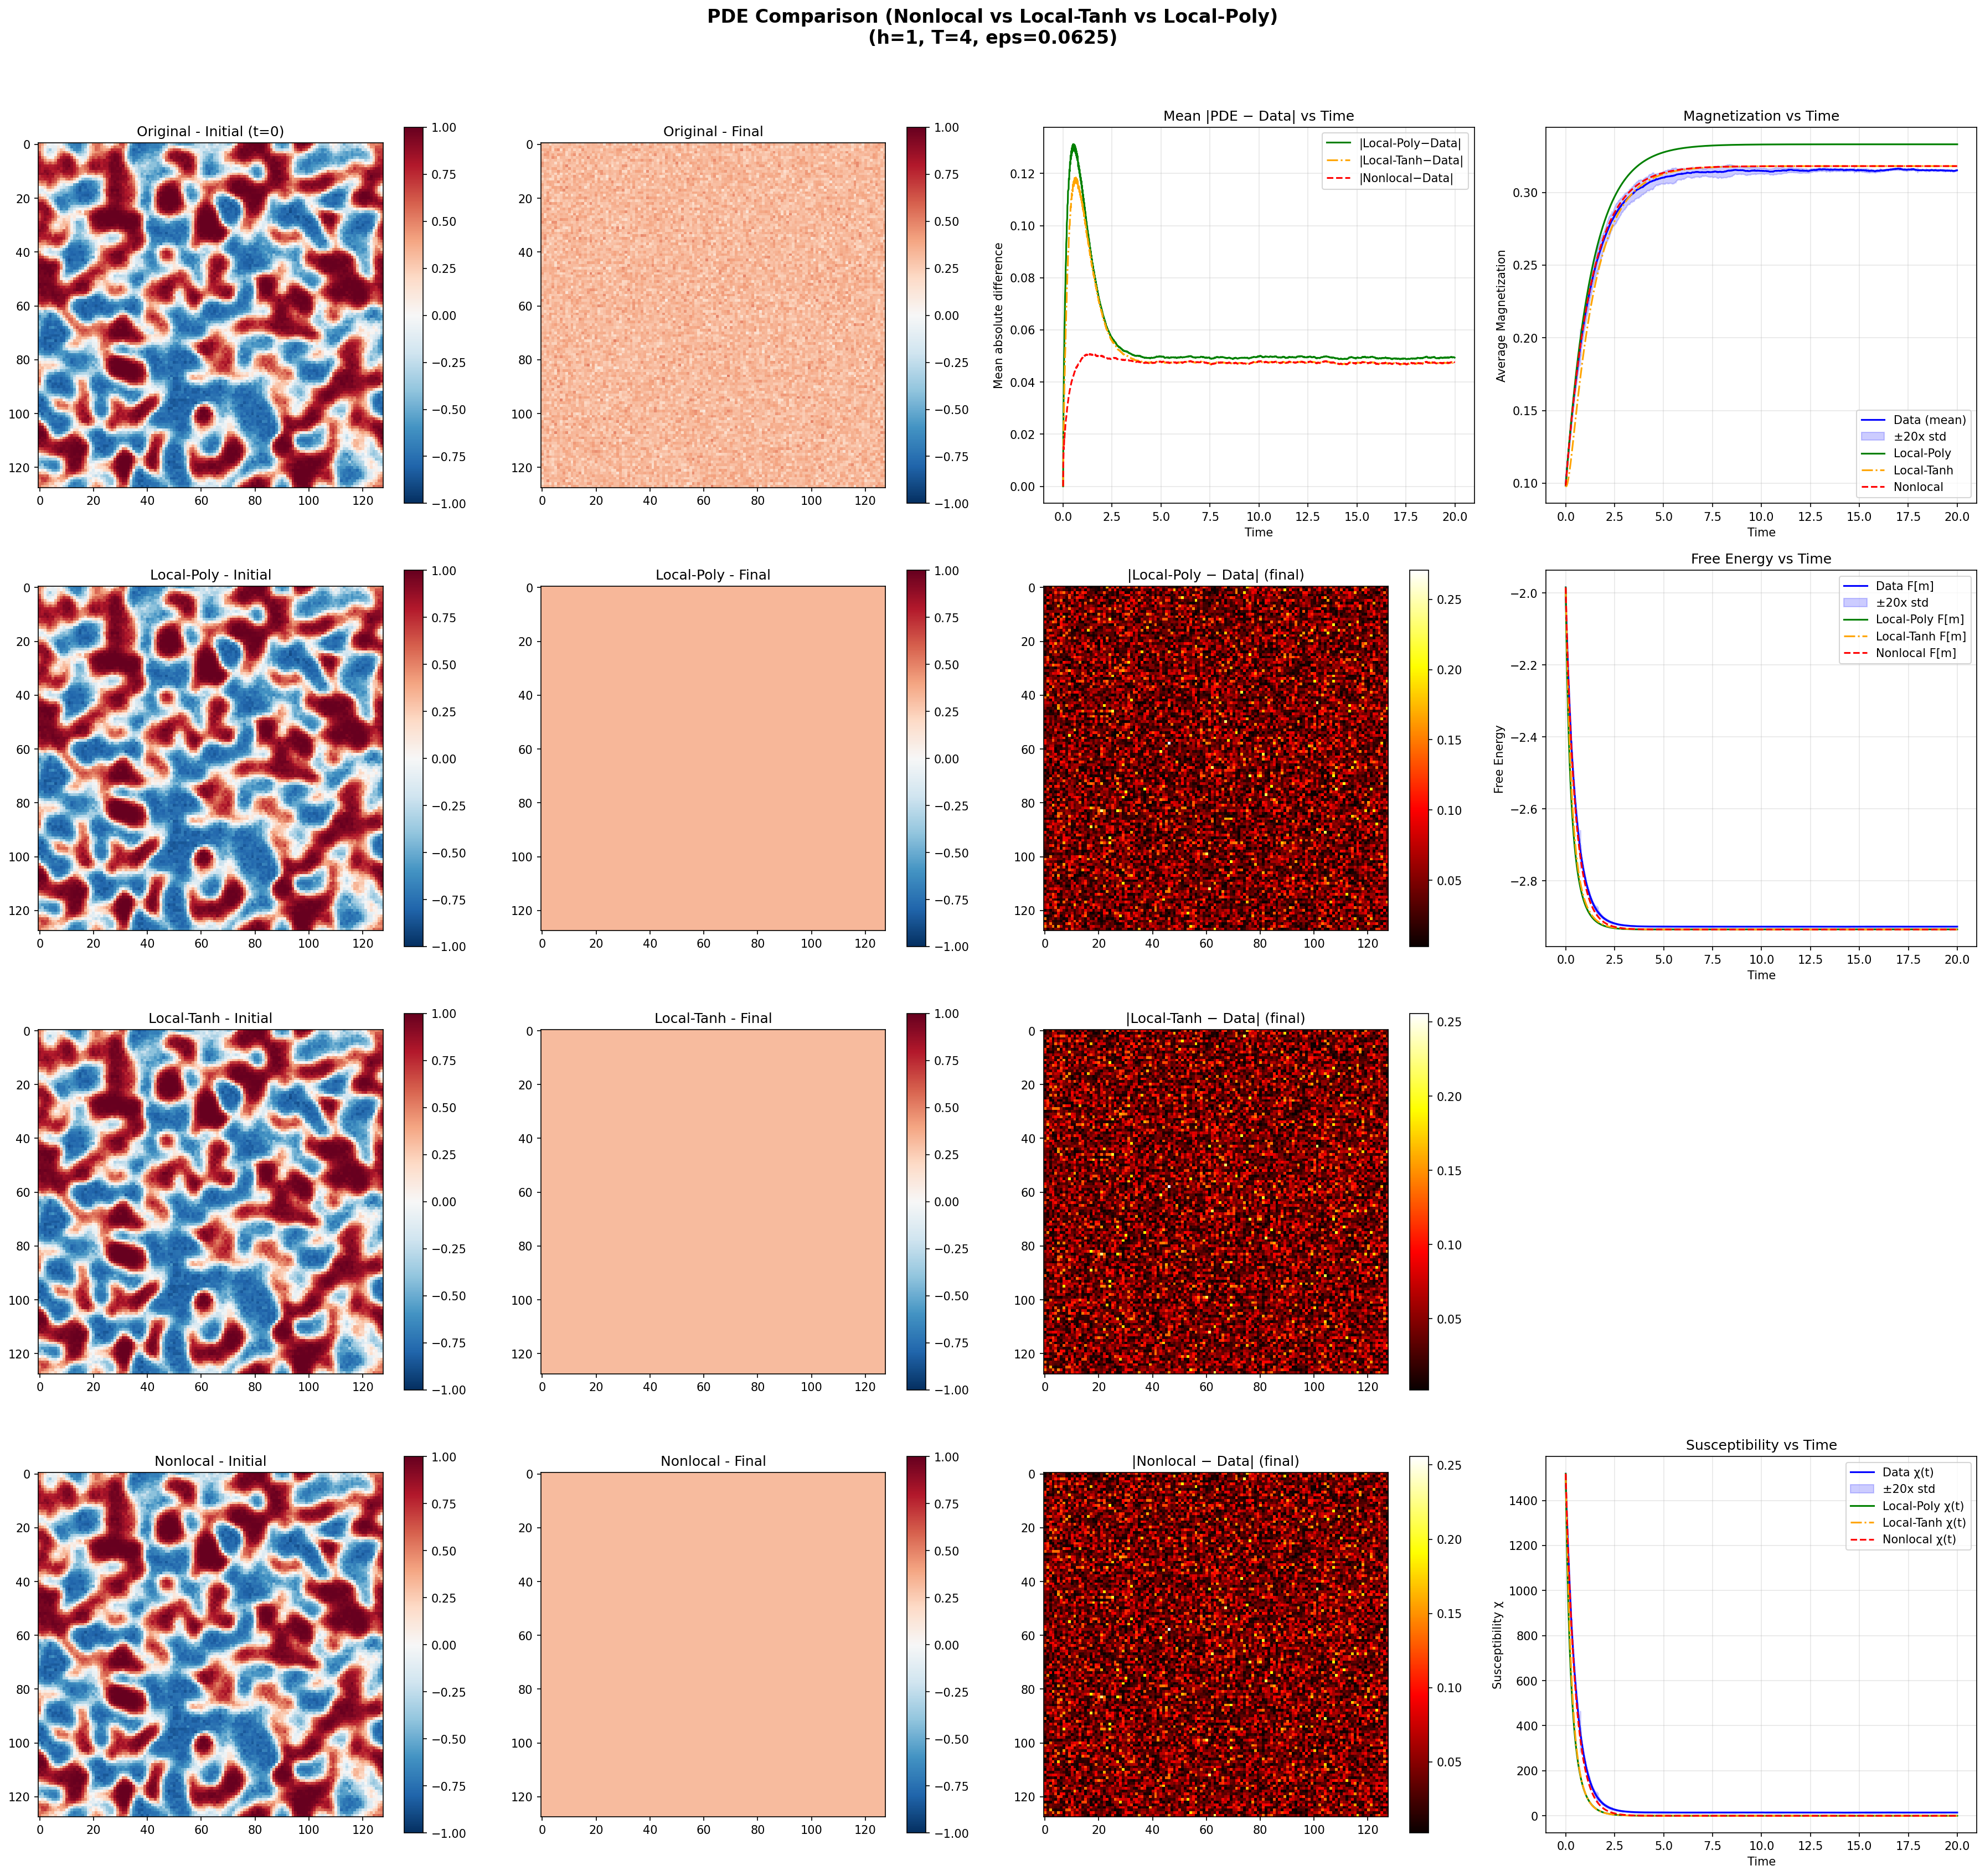
\includegraphics[width=1.0\textwidth]{fig/compare_pde_solvers_L2048_h1_T4_eps0.0625.png}
% 	\caption{Comparison of original data and PDE solutions for $h=1$, $T=4$, $\epsilon=0.0625$, $L=2048$.}
% 	\label{fig:pde_comparison_h1_T4_eps0.0625_L2048}
% \end{figure}


% % ------------------------------------------------------------
% \subsection{Error metric and statistical indicators used in comparisons}
% \label{sec:error_and_stats}

% We summarize the precise definitions of the error curves and the three statistical indicators displayed in the comparison figures (data, local PDE, nonlocal PDE). We work on the periodic domain $\Omega=[0,1]^2$ discretized by an $M\times M$ grid with spacing $\Delta x = \Delta y = 1/M$ and $N=M^2$ grid points. Spatial integrals are approximated by Riemann sums with weight $\Delta x\,\Delta y = 1/M^2$.

% \paragraph{Time alignment.} Let $\{t^{\text{data}}_n\}_{n=0}^{T_{\text{data}}-1}$, $\{t^{\text{loc}}_n\}_{n=0}^{T_{\text{loc}}-1}$ and $\{t^{\text{non}}_n\}_{n=0}^{T_{\text{non}}-1}$ denote the sampled times for the data, local PDE, and nonlocal PDE trajectories, respectively. For plotting time series jointly, we form a common index set of length $T_\ast=\min(T_{\text{data}},T_{\text{loc}},T_{\text{non}})$ by taking linearly spaced integer indices into each sequence (nearest-neighbor subsampling). We denote the aligned fields by $m_{\text{data}}(t_i,\cdot)$, $m_{\text{loc}}(t_i,\cdot)$, and $m_{\text{non}}(t_i,\cdot)$ for $i=0,\dots,T_\ast-1$.

% \paragraph{Magnetization (spatial mean).} For any field $m(t,\cdot)$,
% \begin{equation}
% 	\overline{m}(t) \;=\; \frac{1}{|\Omega|} \int_{\Omega} m(t,\mathbf{x})\,d\mathbf{x}
% 	\;\approx\; \frac{1}{M^2} \sum_{i,j=0}^{M-1} m_{i,j}(t).
% \end{equation}
% We plot $\overline{m}_{\text{data}}(t_i)$, $\overline{m}_{\text{loc}}(t_i)$, and $\overline{m}_{\text{non}}(t_i)$ on a shared time axis.

% \paragraph{Free energy used in plots (post-processing functional).} Let $\beta>0$ be the inverse temperature, $h\in\mathbb{R}$ the external field, $J_0\in\mathbb{R}$ an interaction-strength factor, and $J$ a nonnegative, radially symmetric, \emph{sum-normalized} kernel (i.e., the discrete sum of $J$ over the periodic grid equals one). Define $p=(1+m)/2$ and $q=(1-m)/2$. The free energy density used in the plots is
% \begin{equation}
% 	f(m) \;=\; \frac{1}{\beta}\Big( p\,\ln p + q\,\ln q \Big)
% 	\; -\; \frac{J_0}{2}\, m\, (J*m)
% 	\; -\; h\, m,
% \end{equation}
% and the post-processed free energy is
% \begin{equation}
% 	F[m](t) \;=\; \int_{\Omega} f\big(m(t,\mathbf{x})\big)\,d\mathbf{x}
% 	\;\approx\; \frac{1}{M^2} \sum_{i,j=0}^{M-1} \Bigg[ \frac{1}{\beta}\Big( p_{i,j}\ln p_{i,j} + q_{i,j}\ln q_{i,j} \Big)
% 		- \frac{J_0}{2}\, m_{i,j}\, (J*m)_{i,j}
% 		- h\, m_{i,j} \Bigg].
% \end{equation}
% Here $(J*m)$ is the \emph{periodic} convolution of $m$ with $J$ on the $M\times M$ grid; in computations it is obtained by constructing $J$ in real space, normalizing to unit discrete sum, applying $\mathrm{ifftshift}$, taking its $\mathrm{fft2}$, and multiplying in Fourier space before an inverse FFT.

% \emph{Remark.} This plotted functional differs from the theoretical Lyapunov functional in \cref{sec:nonlocal_theory} by constant shifts and scaling conventions (e.g., factors of $\beta$ and $J_0$); it is chosen to match the numerical post-processing used across data/local/nonlocal trajectories.

% \paragraph{Magnetic susceptibility.} The spatial susceptibility is computed as
% \begin{equation}
% 	\chi(t) \;=\; \beta\,N\,\Big( \langle m^2(t,\cdot)\rangle_x - \langle m(t,\cdot)\rangle_x^{\,2} \Big),
% \end{equation}
% where $\langle\cdot\rangle_x$ denotes the spatial average over the grid, i.e., $\langle m\rangle_x = M^{-2}\sum m_{i,j}$ and $N=M^2$. We plot $\chi_{\text{data}}(t_i)$, $\chi_{\text{loc}}(t_i)$, and $\chi_{\text{non}}(t_i)$ on a shared time axis.

% \paragraph{Cross-resolution comparability.} In resolution studies where trajectories are available on different grids $M$, we first resample all fields onto a common \emph{reference grid} (the data grid) using \emph{periodic bilinear interpolation} before computing spatial averages and functionals (\,$\overline m(t)$, $\chi(t)$, $F[m](t)$\,) and before forming error curves. This removes spurious resolution dependence from the factor $N=M^2$ and from discretization effects, ensuring that, for example, $\chi(0)$ is directly comparable across resolutions.

% \paragraph{Energy convention in plots.} To compare data and PDE on equal footing, the energy-like panel uses the \emph{same post-processed free energy} $F[m](t)$ for both data and PDE, computed from the functional above with identical kernel normalization and parameters. When precomputed $F$ is unavailable in the data files, we recompute $F[m]$ from the stored coarse-grained fields. We intentionally avoid plotting the internal energy $E$ alone, since it omits the entropic term and can differ by constant/scaling factors; $F[m]$ provides a consistent, physically meaningful comparison across methods and resolutions.

% \paragraph{Mean absolute error curves.} The error curves shown are the \emph{spatial mean absolute error} between PDE solutions and data at aligned times:
% \begin{equation}
% 	E_{\text{loc}}(t_i) \;=\; \frac{1}{M^2} \sum_{k,\ell=0}^{M-1} \big|\, m_{\text{loc};\,k\ell}(t_i) - m_{\text{data};\,k\ell}(t_i) \,\big|,
% 	\qquad
% 	E_{\text{non}}(t_i) \;=\; \frac{1}{M^2} \sum_{k,\ell=0}^{M-1} \big|\, m_{\text{non};\,k\ell}(t_i) - m_{\text{data};\,k\ell}(t_i) \,\big|.
% \end{equation}
% These correspond to the $\textit{Mean $|\mathrm{PDE}-\mathrm{Data}|$ vs Time}$ panel.

% \subsection{Main Findings from PDE Comparisons}
% \label{subsec:main_findings}
% We summarize the main findings from the PDE comparison experiments.
% First, as the lattice size $L$ increases, the standard deviation of the magnetization decreases
% (as illustrated in the three pairs of figures:
% \cref{fig:pde_comparison_h0_T1_eps0.015625,fig:pde_comparison_h0_T1_eps0.015625_L2048},
% \cref{fig:pde_comparison_h0_T4_eps0.015625,fig:pde_comparison_h0_T4_eps0.015625_L2048},
% and \cref{fig:pde_comparison_h1_T4_eps0.015625,fig:pde_comparison_h1_T4_eps0.015625_L2048}).
% This observation is consistent with the theoretical results : as $L \to \infty$, the fluctuations of the empirical magnetization vanish and the empirical magnetization converges to the solution of the hydrodynamic limit PDE.

% Second, the local PDE with $\tanh$ form and with simplified polynomial form (Allen-Cahn) both provide good approximations to the microscopic dynamics when the kernel range $\epsilon$ is small (e.g., $\epsilon=2\delta$ and $\epsilon=4\delta$).
% However, as $\epsilon$ increases (e.g., $\epsilon=8\delta$), the nonlocal PDE consistently outperforms the local PDEs in terms of accuracy.
% This is particularly evident in the low-temperature regime ($T=1$) with zero external field ($h=0$), where the local PDEs struggle to capture the intricate domain structures formed during phase separation (as shown in \cref{fig:pde_comparison_h0_T1_eps0.0625,fig:pde_comparison_h0_T1_eps0.0625_L2048}).
% In contrast, the nonlocal PDE effectively captures these structures, leading to significantly lower error metrics.
% Also, the local PDE with $\tanh$ form generally outperforms the Allen-Cahn equation.

% Third, at low temperature ($T=1$) with a narrow kernel ($\epsilon = 2\delta$)
% (see \Cref{fig:pde_comparison_h0_T1_eps0.015625,fig:pde_comparison_h0_T1_eps0.015625_L2048}),
% the non-local PDE approximation performs worse than the local Allen-Cahn model.
% This discrepancy is most likely due to numerical errors in evaluating the discrete convolution with such a narrow kernel,
% as the data are generated on a fine lattice while the non-local PDE is solved on a coarser grid.
% As the kernel range increases, these convolution errors diminish.
% A quantitative comparison of errors for different kernel ranges is provided in \Cref{tab:convolution_error}.

% \begin{table}
% 	\centering
% 	\begin{tabular}{lllll}
% 		\hline
% 		\hline
% 		\textbf{$\epsilon$} & $1\delta$ & $2\delta$ & $4\delta$ & $8\delta$ \\
% 		\hline
% 		Convolution Error   & 0.003111  & 0.001017  & 0.000366  & 0.000135  \\
% 		\hline
% 		\hline
% 	\end{tabular}
% 	\caption{Comparison of discrete convolution error with different kernel range $\epsilon$. The convolution error is calculated as the mean absolute error between the discrete convolution on a $1024\times 1024$ lattice and the coarse-grained $128 \times 128$ lattice, averaged over 20 random magnetization fields.}
% 	\label{tab:convolution_error}
% \end{table}

% \subsection{Numerical stability and CFL considerations (local PDE with RK4)}
% \label{subsec:numerical_cfl}

% This section summarizes the numerical stability constraints observed in our resolution study for the \emph{local} PDE solvers (both the Allen--Cahn polynomial form and the local-limit tanh form), and clarifies how we ensure consistent comparisons across resolutions.

% \paragraph{Root cause.} The local PDEs include a diffusion term $\kappa\,\Delta m$. When integrated with explicit Runge--Kutta (RK) methods, the stable time step is limited by the highest resolvable spatial frequency on the grid. On a periodic $M\times M$ grid with $\Delta x=\Delta y=L/M$, a conservative characterization of the largest Laplacian eigenvalue is
% \[
% 	k_\text{max}^2 \;\approx\; \Big(\tfrac{\pi}{\Delta x}\Big)^2 + \Big(\tfrac{\pi}{\Delta y}\Big)^2\,.
% \]
% For the linear test problem $u_t=\kappa\,\Delta u$, explicit RK4 is stable provided $\Delta t\,\kappa\,k_\text{max}^2$ lies within RK4's stability region along the negative real axis. Using the known stability bound $\alpha_\text{RK4}\approx 2.785$ and a safety factor $s\in(0,1)$, we enforce the limiter
% \begin{equation}
% 	\Delta t_\text{eff} \;=\; \min\!\left( \Delta t_\text{in},\; s\,\frac{\alpha_\text{RK4}}{\kappa\,k_\text{max}^2} \right),
% 	\qquad k_\text{max}^2\approx \Big(\tfrac{\pi}{\Delta x}\Big)^2+\Big(\tfrac{\pi}{\Delta y}\Big)^2,\;\; s\approx 0.5.
% 	\label{eq:rk4_cfl}
% \end{equation}
% Because $k_\text{max}^2\propto M^2$, the admissible time step scales like $\Delta t_\text{eff}\propto 1/M^2$. Hence, merely refining the grid (e.g., from $M=128$ to $M=256$) without reducing $\Delta t$ leads to instability or severe phase/dissipation errors.

% \paragraph{Implementation in our solvers.} We enforce \eqref{eq:rk4_cfl} in the local solver at runtime:
% \begin{itemize}
% 	\item Compute $\Delta t_\text{eff}$ via \eqref{eq:rk4_cfl} using the current $\kappa$, $M$, and domain size $L$.
% 	\item Keep the \emph{physical horizon} $t_\text{end}$ fixed by rescaling the number of steps as $N_\text{steps}=\lceil t_\text{end}/\Delta t_\text{eff}\rceil$.
% 	\item Record at the same cadence in physical time by adjusting the recording frequency accordingly.
% \end{itemize}
% This preserves the comparison across resolutions while ensuring stability as $M$ increases.

% \paragraph{Consistent post-processing across resolutions.} For resolution comparisons, we always resample PDE fields onto the \emph{data grid} (via periodic bilinear interpolation) \emph{before} computing statistics (magnetization, susceptibility, and the post-processed free energy $F[m]$), as well as before forming error curves. This removes spurious $M$-dependent factors (e.g., $N=M^2$ in $\chi$) and discretization discrepancies, yielding directly comparable curves at $t=0$ and beyond.

% \paragraph{Planned results to display.} To illustrate the effect and the fix, we will show:
% \begin{enumerate}
% 	\item A baseline at $M=128$ ($\Delta x=1/128$) with input time step $\Delta t_\text{in}=10^{-2}$. This case is stable and serves as reference.
% 	\item A naive refinement to $M=256$ using the \emph{same} $\Delta t_\text{in}=10^{-2}$ (no limiter): the solution exhibits instability/visible artifacts (divergence or severe distortion), confirming the $\propto 1/M^2$ constraint.
% 	\item The corrected $M=256$ run with the RK4 diffusion limiter \eqref{eq:rk4_cfl} enabled (thus $\Delta t_\text{eff}$ reduced by a factor $\approx4$): the evolution becomes stable and compares consistently with the $M=128$ reference.
% 	\item Optionally, a further refinement to $M=512$, again with \eqref{eq:rk4_cfl}, demonstrating that results remain stable as the grid is refined when $\Delta t$ scales properly.
% \end{enumerate}
% For each setting we will show the standard 4-row comparison panel (data snapshots, error vs time, magnetization vs time, and the unified free-energy and susceptibility time series), with consistent post-processing on the data grid.

% \subsubsection{CFL time step calculation for specific parameter combinations}

% For concrete illustration, we analyze the CFL limits for the parameter sets used in our computational experiments. Using \eqref{eq:rk4_cfl} with domain size $L=1$ and typical diffusion coefficient $\kappa \approx 0.1$ estimated from the Allen-Cahn parameters:

% In both parameter regimes, the naive choice $\Delta t = 0.01$ leads to severe CFL violations at fine spatial resolutions, explaining the numerical instabilities observed when CFL enforcement is disabled. The required stable time steps are 1-2 orders of magnitude smaller than commonly assumed, making automatic CFL limiting essential for robust simulations.

% \paragraph{Actual time steps used with CFL enforcement} Our implementation uses the formula
% \[
% 	\Delta t_\text{eff} = \min\!\left( \Delta t_\text{in},\; \frac{s \times \alpha_\text{RK4}}{\kappa \times k_\text{max}^2} \right)
% \]
% with safety factor $s = 0.5$, stability constant $\alpha_\text{RK4} = 2.785$, and diffusion coefficient $\kappa = 0.5 \beta J_0 \epsilon^2 \approx 0.5 \times 1 \times 1 \times (0.0625)^2 \approx 0.00195$. For the specific cases:

% \paragraph{Case 1: $h=0$, $T=1$, $\epsilon=0.0625$}
% \begin{itemize}
% 	\item $N=128$: $\Delta t_\text{eff} = \min(0.01, 2.21 \times 10^{-3}) = 2.21 \times 10^{-3}$ (CFL-limited by factor 4.5)
% 	\item $N=256$: $\Delta t_\text{eff} = \min(0.01, 5.51 \times 10^{-4}) = 5.51 \times 10^{-4}$ (CFL-limited by factor 18.1)
% \end{itemize}

% \paragraph{Case 2: $h=1$, $T=4$, $\epsilon=0.0625$}
% \begin{itemize}
% 	\item $N=128$: $\Delta t_\text{eff} = \min(0.01, 2.21 \times 10^{-3}) = 2.21 \times 10^{-3}$ (CFL-limited by factor 4.5)
% 	\item $N=256$: $\Delta t_\text{eff} = \min(0.01, 5.51 \times 10^{-4}) = 5.51 \times 10^{-4}$ (CFL-limited by factor 18.1)
% \end{itemize}

% These effective time steps ensure numerical stability while maintaining the same physical simulation time $t_\text{end} = 20.0$ by automatically increasing the number of integration steps as needed.

% We show the CFL study for the local PDE with RK4 for $h=0$, $T=1$, $\epsilon=0.0625$ and $h=1$, $T=4$, $\epsilon=0.0625$ in \cref{fig:pde_cfl_study_h0_T1_eps0.0625} and \cref{fig:pde_cfl_study_h1_T4_eps0.0625}.

% \begin{figure}[!h]
% 	\centering
% 	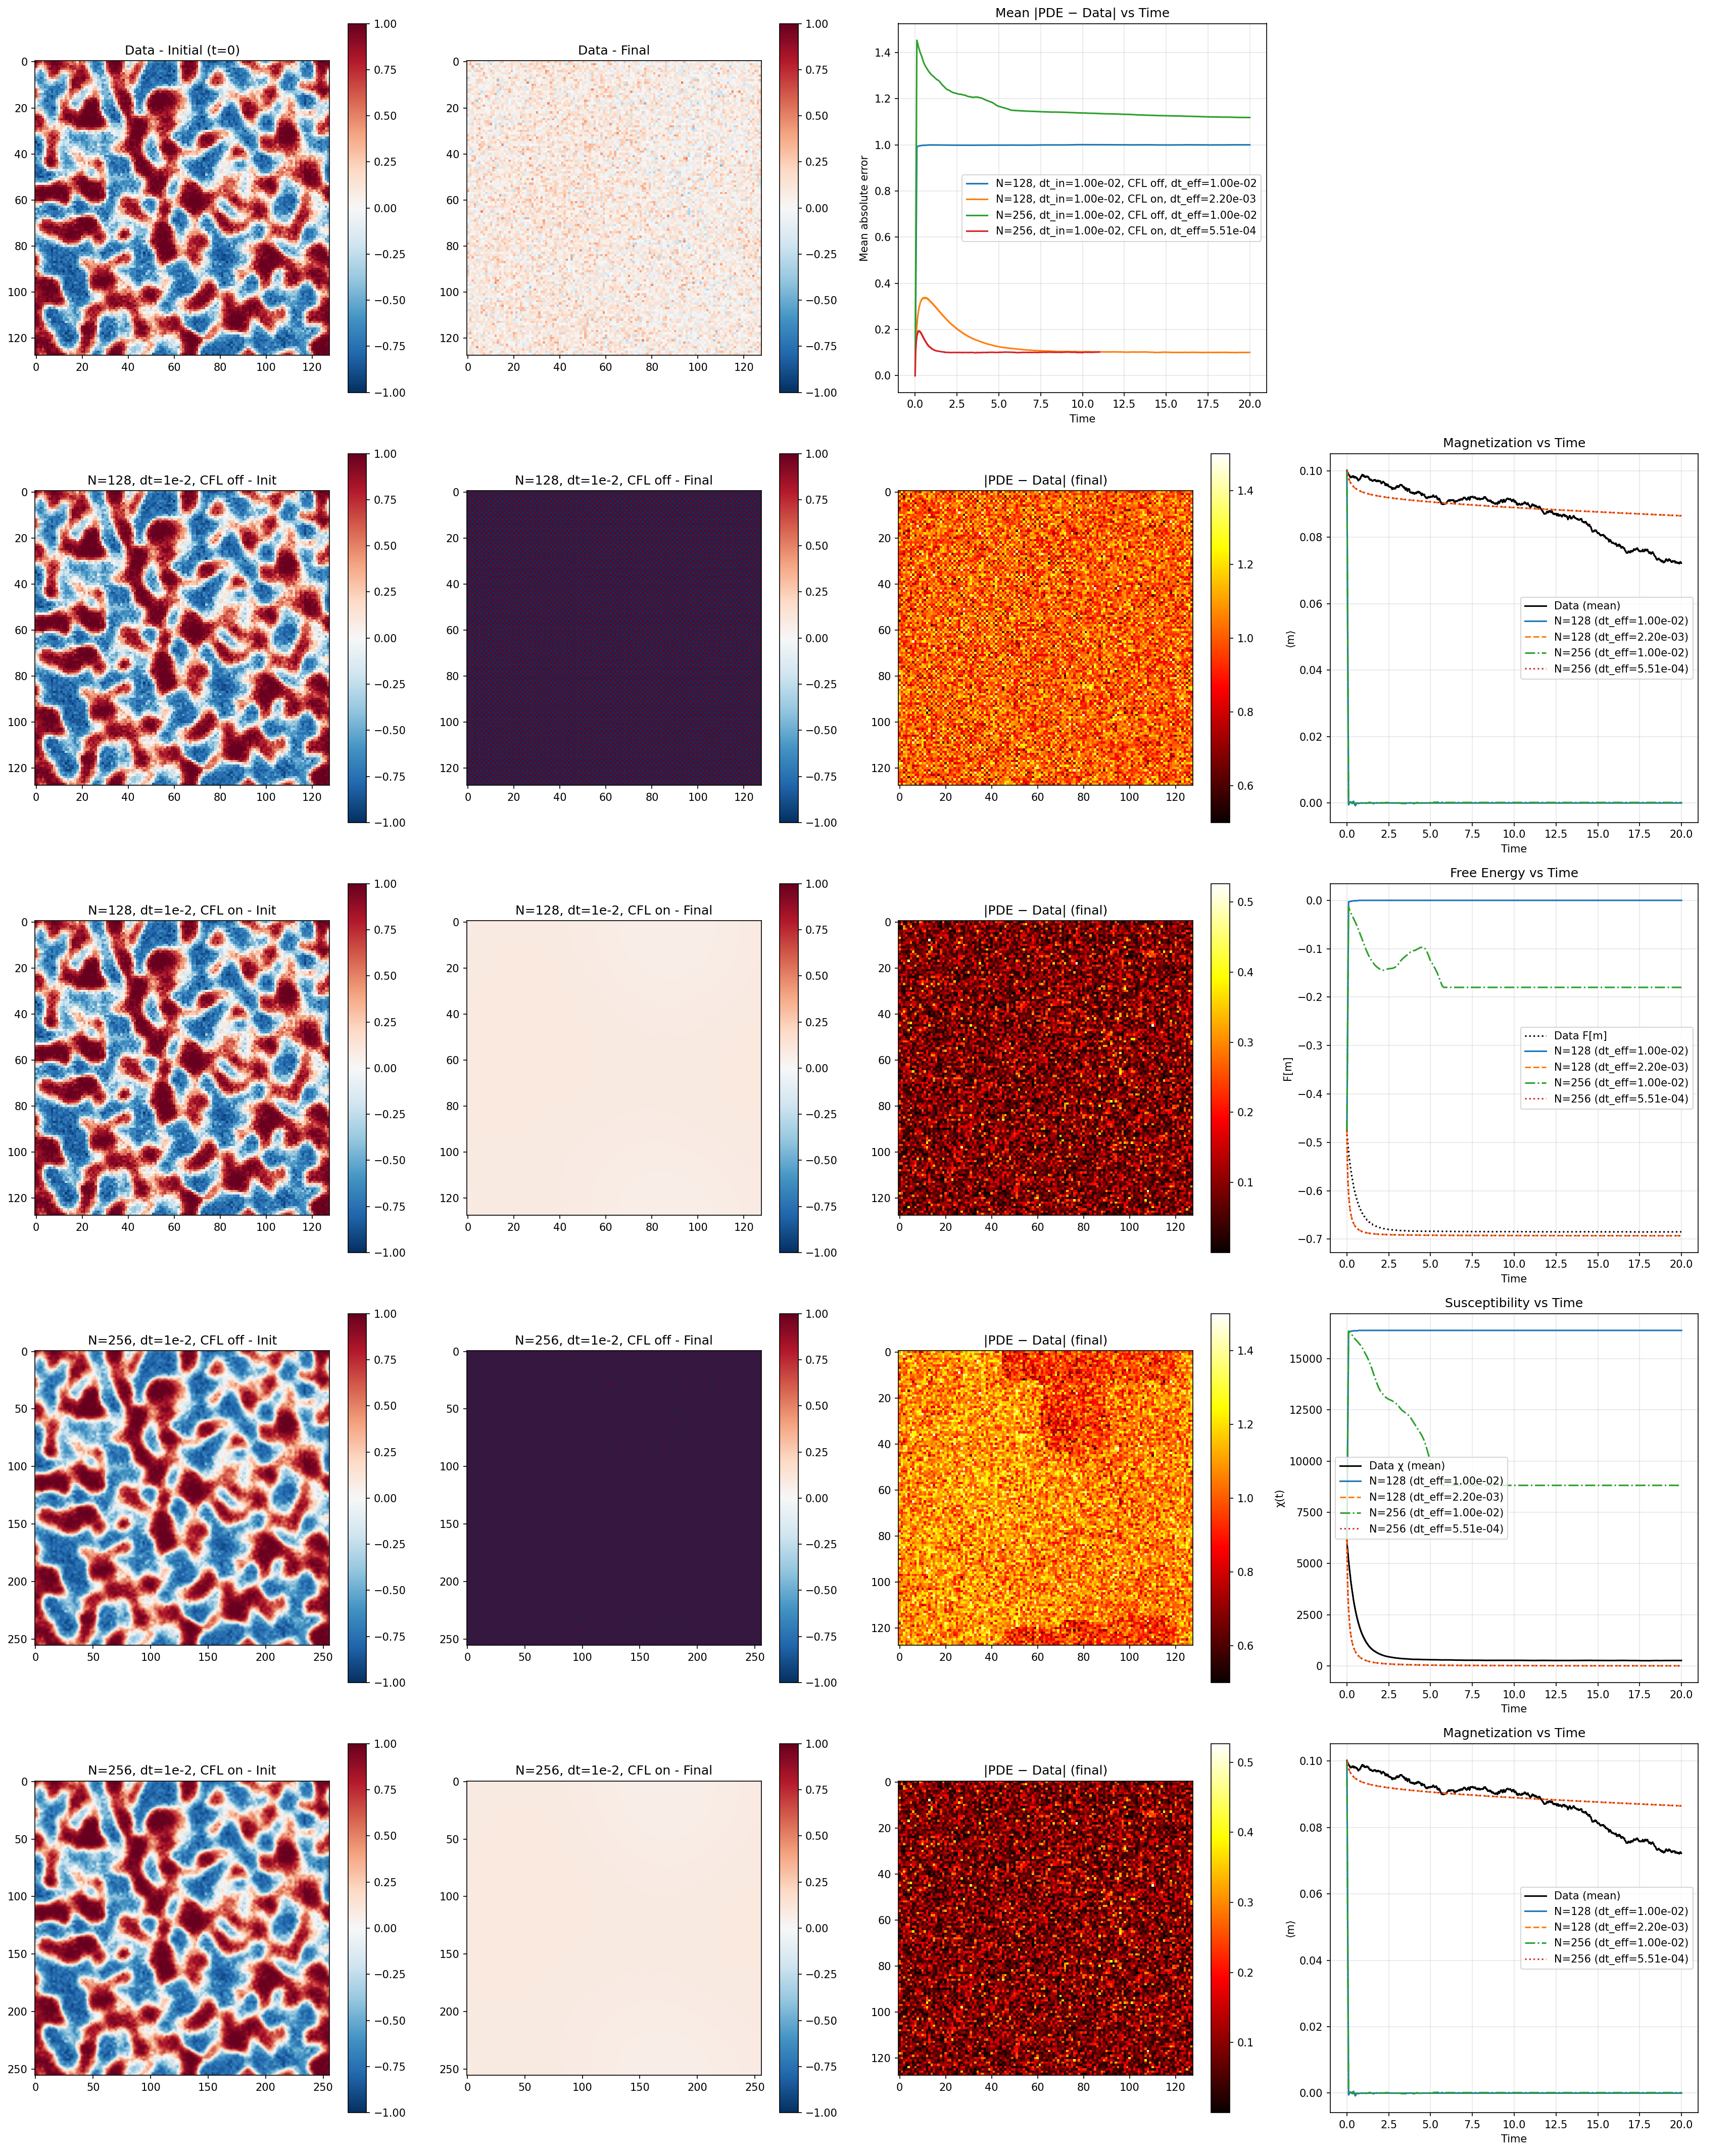
\includegraphics[width=1.0\textwidth]{fig/pde_cfl_study_poly_h=0_T=1_eps=0.0625_L=1024.png}
% 	\caption{CFL study for the local PDE with RK4 for $h=0$, $T=1$, $\epsilon=0.0625$.}
% 	\label{fig:pde_cfl_study_h0_T1_eps0.0625}
% \end{figure}

% \begin{figure}[!h]
% 	\centering
% 	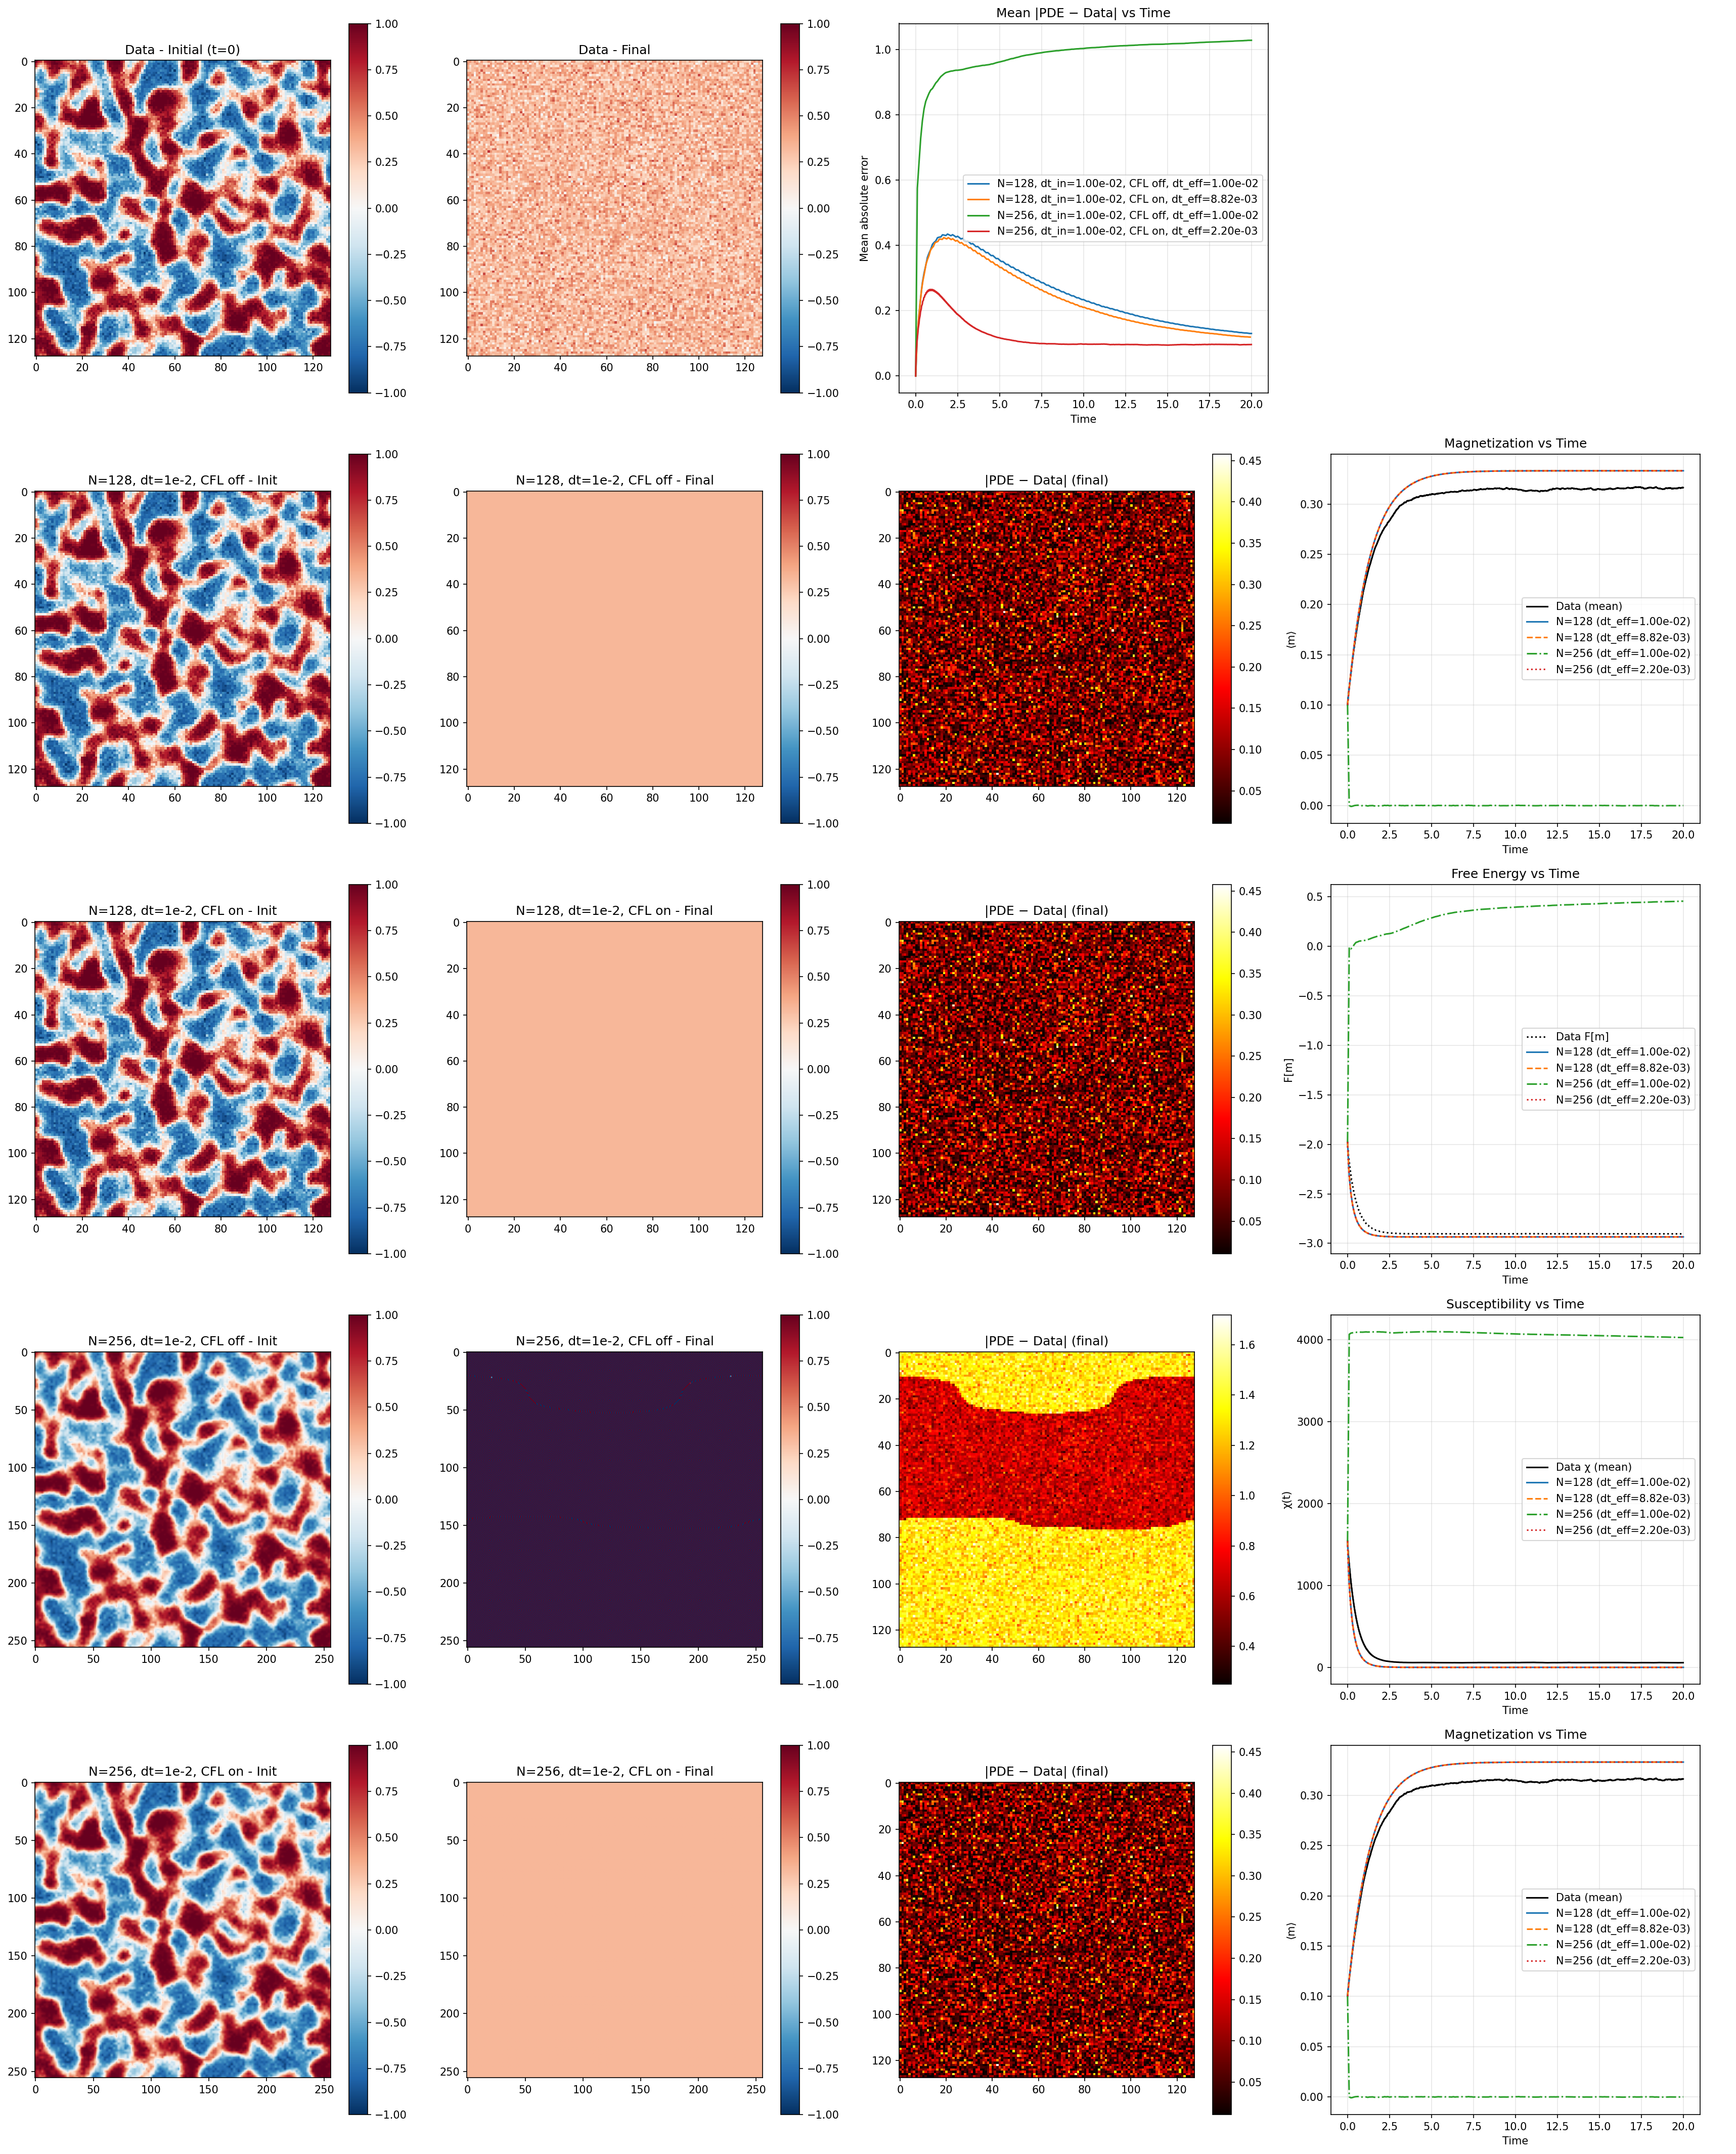
\includegraphics[width=1.0\textwidth]{fig/pde_cfl_study_poly_h=1_T=4_eps=0.0625_L=1024.png}
% 	\caption{CFL study for the local PDE with RK4 for $h=1$, $T=4$, $\epsilon=0.0625$.}
% 	\label{fig:pde_cfl_study_h1_T4_eps0.0625}
% \end{figure}



% \section{Network Training}
% \label{sec:network}

% \subsection{Motivation}
% The hydrodynamic limit derived in \cref{subsec:hydro} leads to the mesoscopic PDE
% \begin{equation}
% 	\partial_t m(t,x) = -m(t,x) + \tanh\!\big(\beta (J_\epsilon \ast m)(t,x) + \beta h \big),
% 	\quad m(0,x) = m_0(x).
% 	\label{eq:hydro}
% \end{equation}
% This deterministic equation provides the baseline dynamics for coarse-grained magnetization.
% However, the precise form of the interaction kernel $J_\epsilon$ and the functional dependence of
% the nonlinear force may not be directly available in practical systems.
% To bridge this gap, we explore neural-network parameterizations of the generator of the dynamics.

% \subsection{Network Parameterizations}
% We consider two levels of prior knowledge.

% \paragraph{Strong prior (physics-informed).}
% We constrain the force to have the form
% \begin{equation}
% 	F(I,m,h) = -A m + \tanh(BI + C m + D h),
% 	\label{eq:strong_prior}
% \end{equation}
% where $I=(J_\theta \ast m)(x)$ denotes the nonlocal interaction term computed via a learnable kernel $J_\theta$,
% and $A,B,C,D$ are trainable parameters.
% This corresponds exactly to the \texttt{ForceTanhNet} architecture in our implementation.

% \paragraph{Weak prior (black-box MLP).}
% We also test a more flexible model
% \begin{equation}
% 	F_\theta(I,m,h) = \text{MLP}_\theta(I,m,h),
% \end{equation}
% where $\text{MLP}_\theta:\mathbb{R}^3 \to \mathbb{R}$ is a fully connected network with hidden layers (e.g.\ 3 layers, width 128, $\tanh$ activations).
% This allows the network to discover nonlinear dependencies directly from data, at the expense of interpretability.

% \subsection{Learnable Kernels}
% The convolutional operator $I_\theta = J_\theta \ast m$ is implemented by parameterized kernels constrained to be nonnegative and sum to one.
% We investigate three families:
% \begin{itemize}
% 	\item \textbf{Softmax kernel:} a fully learnable $K\times K$ kernel with entries parameterized by logits, normalized by softmax.
% 	\item \textbf{Gaussian kernel:} isotropic Gaussian with learnable variance parameter.
% 	\item \textbf{Elliptical Gaussian kernel:} anisotropic Gaussian with learnable $(\sigma_x, \sigma_y, \theta)$.
% \end{itemize}
% These architectures ensure physical consistency (positivity, normalization) while allowing different degrees of flexibility.

% \subsection{Training Objective}
% Given observed trajectories $\{m_{\text{obs}}(t_i,\cdot)\}$ from microscopic simulations,
% we train the network by minimizing the one-step prediction error of the generator:
% \begin{equation}
% 	\min_{\theta} \sum_{m \in \mathcal{D}}
% 	\left\| L_\theta(m) - \partial_t m_{\text{obs}} \right\|_{L^2(\Omega)}^2,
% 	\label{eq:training}
% \end{equation}
% where
% \begin{equation}
% 	L_\theta(m) = F_\theta(I_\theta(m), m, h).
% \end{equation}
% The time derivatives $\partial_t m_{\text{obs}}$ are estimated from data either by finite differences or regression.

% \subsection{Implementation Details}
% \begin{itemize}
% 	\item \textbf{Input representation:} magnetization fields $m$ are coarse-grained to size $M\times M$.
% 	      At each training step, we sample random spatial coordinates $(x,y)$ and evaluate both $I_\theta(m)$ and $m(x,y)$ using periodic convolution (global evaluation) or local patch sampling.
% 	\item \textbf{Loss computation:} prediction $L_\theta(m)$ is compared against the empirical $\partial_t m$ at the same coordinates.
% 	\item \textbf{Optimization:} networks are trained with Adam optimizer, learning rate $10^{-3}$, and batch size 16.
% \end{itemize}

% \subsection{Planned Experiments}
% The following experiments are included:
% \begin{enumerate}
% 	\item \textbf{Strong vs weak prior:} compare \eqref{eq:strong_prior} with unconstrained MLPs in terms of predictive accuracy and generalization.
% 	\item \textbf{Kernel families:} test softmax, Gaussian, and elliptical Gaussian kernels for learning effective interaction structures.
% 	\item \textbf{Generalization across regimes:} train at high temperature ($T > T_c$) and evaluate at low temperature ($T < T_c$), and vice versa.
% 	\item \textbf{Comparison with PDE models:} evaluate learned generators against the original hydrodynamic PDE \eqref{eq:nonlocal} and its local Allen–Cahn approximation.
% \end{enumerate}
% This systematic study will assess how inductive bias and kernel parameterization influence both accuracy and interpretability of learned mesoscopic models.


\section{Regularity and well-posedness for learned nonlocal dynamics}
\label{sec:network_regularity}
\subsection{Outline}


Recall the physical mesoscopic PDE on the periodic domain $\Omega=\mathbb{T}^d$:
\[
	\partial_t m(t,x) \;=\; -\,m(t,x)\; +\; \tanh\!\big(\beta\,((J_\epsilon * m)(t,x) + h)\big),
	\qquad m(0,\cdot)=m_0(\cdot).
\]
Here $J_\epsilon$ is nonnegative, even, and sum-normalized (discrete: unit-sum; continuum: $\int_\Omega J_\epsilon=1$). We have $m_0\in L^\infty(\Omega)$ with $\|m_0\|_{L^\infty}\le 1$. Also, $I = (J_\epsilon * m) \in [-1,1]$ whenever $m\in [-1,1]$.


% We analyze the regularity and stability of the \emph{learned} generator that appears in the network training part, in the setting of the mesoscopic Ising/Glauber hydrodynamics. Throughout we work on the periodic domain $\Omega=\mathbb{T}^d$ ($d=2$ in our experiments). Let
% \[
% 	\partial_t m(t,\mathbf{x}) \;=\; L_\theta[m](t,\mathbf{x})
% 	\;:=\; F_\theta\big( (J_\theta * m)(t,\mathbf{x}),\; m(t,\mathbf{x}),\; h \big),
% 	\qquad m(0,\cdot)=m_0(\cdot),
% \]
% where $J_\theta$ is a nonnegative, sum-normalized interaction kernel and $F_\theta$ is a parametric nonlinearity. Two concrete parameterizations used in our implementation are:

% - \textbf{Strong prior (physics-informed), cf.~\eqref{eq:strong_prior}}:
% \[
% 	F_\theta(I,m,h) = -A m + \tanh(B I + C m + D h),
% \]
% which reduces to the Glauber--Kac form when $(A,B,C,D)=(1,\beta,0,\beta)$ and $I=(J * m)$.

% - \textbf{Black-box MLP}: $F_\theta(I,m,h)=\mathrm{MLP}_\theta(I,m,h)$ with smooth activations (e.g., $\tanh$), used in \S\ref{sec:network}.

% We establish well-posedness, invariant bounds, and propagation of Sobolev regularity for this evolution, and provide stability/error estimates comparing the learned generator $L_\theta$ with the physical generator
% \[
% 	L_\ast[m] \;=\; -m + \tanh\!\big( \beta (J_\epsilon * m + h) \big),
% \]
% cf.~\eqref{eq:hydro}.


We aim to learn networks to approximate the target dynamics/generator
$$
	\partial_t m = \mathcal{F}[m] = \mathcal{F}_\theta\big(\mathcal{I}_{\theta\prime}[m], m, h \big),
$$
where the interaction term is $\mathcal{I}_{\theta\prime}[m]=(J_{\theta\prime}*m)$; more generally $\mathcal{I}_{\theta\prime}$ can be the state-dependent operator in \S\ref{subsec:state_dependent_J}.

We now specify different priors. We specify the priors on $(\mathcal{F}_\theta,J_{\theta\prime})$.
\begin{itemize}
	\item For nonlinearities, we consider two priors:
	      \begin{itemize}
		      \item \textbf{Strong prior.} $\mathcal{F}_\theta$ is a neural network $\mathrm{MLP}_\theta(I,m,h)$; $J$ is learnable and may be a local convolution kernel $K_\theta(x-y)$ or a state-dependent operator $K_\theta(x,y; m)$ (normalized as in \eqref{eq:state_dep_op}).
		      \item \textbf{Weak prior.} $\mathcal{F}_\theta$ is a neural network $\mathrm{MLP}_\theta(I,m,h)$ (we discuss some specific structures in the following); $J$ is learnable and may be a local convolution kernel $K_\theta(x-y)$ or a state-dependent operator $K_\theta(x,y; m)$ (normalized as in \eqref{eq:state_dep_op}).
	      \end{itemize}
	\item For kernels, we consider three types:
	      \begin{itemize}
		      \item \textbf{Local kernel.} $J_{\theta\prime}$ is a local convolution kernel $K_\theta(x-y)$, which is a fully learnable $K\times K$ kernel with entries parameterized by logits, normalized by softmax. Similar to CNN.
		      \item \textbf{Non-local kernel.} $J_{\theta\prime}$ is a non-local convolution kernel $K_\theta(x,y)$, which is a fully learnable $K\times K$ kernel with entries parameterized by logits, normalized by softmax.
		      \item \textbf{State-dependent kernel, nonlinear operator.} $J_{\theta\prime}$ is a state-dependent operator $K_\theta(x,y; m)$, which is a fully learnable $K\times K$ kernel with entries parameterized by logits, normalized by softmax. Similar to self-attention.
	      \end{itemize}
\end{itemize}


We next specify constraints/regularity on $(\mathcal{F}_\theta,J_{\theta\prime})$ (e.g., positivity/normalization of $J_{\theta\prime}$, locally $p$-Lipschitz $\mathcal{F}_\theta$, and inward-pointing conditions) to ensure well-posedness and stability of the learned flow.


\paragraph{Regularity and well-posedness.}
Given an evolution $\partial_t m = \mathcal{F}[m]$ on a chosen function space $X$ (e.g., $L^\infty(\Omega)$), the common properties one needs to establish are:

\begin{itemize}
	\item \textbf{Boundedness and invariant region:}
	      % write an operator form likr X->TX with T=T(m)
	      there exists a nonempty closed set $B\subseteq X$ such that the solution semigroup $S_t$ generated by $\mathcal{F}$ satisfies $S_t(B)\subseteq B$ for all $t\ge 0$ (forward invariance).

	\item \textbf{Well-posedness (existence/uniqueness/continuous dependence):}
	      If $\mathcal{F}:X\to X$ is locally $p$-Lipschitz in the sense of \Cref{def:locally-p-Lip} (or globally $L^p$-Lipschitz on a forward invariant set $B\subseteq X$), then the IVP admits a unique (local, respectively global on $B$) solution and the solution map $S_t$ depends Lipschitz-continuously on the initial data (with respect to $\|\cdot\|_{L^p}$).


	      %   \item \textbf{Propagation of regularity:} 
	      %   If $m_0\in H^s$ and $\mathcal{F}$ together with convolution/composition closes in $H^s$, then $m(t)\in C([0,T];H^s)\cap C^1([0,T];H^s)$.

	\item \textbf{Stability/error propagation:}
	      If both vector fields are $L^p$-Lipschitz on a forward invariant set $B\subseteq X$ with constant $L$ and the generator discrepancy $\varepsilon_*:=\sup_{m\in B}\|\mathcal{L}_\theta[m]-\mathcal{L}_*[m]\|_{L^p}$ is finite, then, by Grönwall's inequality, for all $t\in[0,T]$,
	      $\|m_\theta(t)-m_*(t)\|_{L^p} \le (\varepsilon_*/L)\,(e^{L t}-1)$.

	\item \textbf{Lyapunov/energy dissipation (if available):}
	      Exhibiting a functional that decreases monotonically along solutions provides evidence of stability and convergence. Only for analytical solutions, not sure the relationship with the network.
\end{itemize}



\begin{definition}[Locally $p$-Lipschitz]\label{def:locally-p-Lip}
	Let $1\le p\le \infty$. For a multivariate functional $G: L^p(\Omega)^n \to L^p(\Omega)^n$, we say that $G$ is \emph{locally $p$-Lipschitz} if for any $u\in L^p(\Omega)^n$ there exist constants $\delta(u)>0$ and $C(u)>0$ such that
	\[
		\|u-v\|_{L^p} < \delta(u)
		\ \Longrightarrow\ \
		\|G(u)-G(v)\|_{L^{\infty}} \le C(u)\,\|u-v\|_{L^p},
		\qquad \forall v\in L^p(\Omega)^n.
	\]
\end{definition}

\begin{remark}
	For $u:\Omega\to\mathbb{R}^n$, we use the vector-valued $L^p$ norm
	\[
		\|u\|_{L^p} \;:=\; \big\|\, |u(\cdot)|_2 \,\big\|_{L^p},
	\]
	where $|\cdot|_2$ is the Euclidean norm in $\mathbb{R}^n$ (any two norms in finite dimensions are equivalent, yielding equivalent norms on $L^p(\Omega)^n$). For $p=\infty$, $\|\cdot\|_{L^{\infty}}$ is the essential supremum.
\end{remark}

% Local Lipschitz implies continuity; global Lipschitz implies linear growth bound.

\paragraph{Assumptions on kernels.}
We assume $J_\theta\in L^1(\Omega)$, $J_\theta\ge 0$, $\int_{\Omega} J_\theta \,d\mathbf{x} = 1$, and $J_\theta$ is even. In the discrete implementation, the learnable kernels (softmax/Gaussian/elliptical Gaussian) are nonnegative and sum to one by construction; in the continuum, these imply that convolution by $J_\theta$ is a bounded linear operator on $L^p(\Omega)$ for all $p\in[1,\infty]$ and on $H^s(\Omega)$ for all $s\in\mathbb{R}$.

\paragraph{Assumptions on nonlinearities.}
For the strong-prior model, $F_\theta$ is globally Lipschitz in $(I,m)$ because $\tanh$ is 1-Lipschitz and the dependence is affine. For MLPs with smooth bounded activations (e.g., $\tanh$), $F_\theta$ is locally Lipschitz everywhere and globally Lipschitz on any bounded set (Rademacher’s theorem in finite dimensions). Since solutions will remain in $(-1,1)$ (see below), this suffices for global existence.





% \begin{theorem}[Global classical well-posedness, invariant region, and equilibria]
% 	\label{thm:nonlocal_wellposed}
% 	Let $d\ge 1$ and $s>\tfrac d2$. Assume $J_\epsilon\in L^1(\Omega)$ is nonnegative, even, and $\|J_\epsilon\|_{L^1}=1$. If $m_0\in H^s(\Omega)$ with $\|m_0\|_{L^\infty}\le 1$, then the nonlocal PDE above admits a unique global solution
% 	\[
% 		m\in C\big([0,\infty);H^s(\Omega)\big)\cap C^1\big([0,\infty);H^s(\Omega)\big),
% 	\]
% 	and the interval $(-1,1)$ is positively invariant: $\|m(t,\cdot)\|_{L^\infty}<1$ for all $t>0$. Moreover, equilibria are exactly the solutions of the nonlinear fixed-point equation
% 	\[
% 		m^*(x) \;=\; \tanh\!\big(\beta\,((J_\epsilon * m^*)(x) + h)\big).
% 	\]
% \end{theorem}

% \begin{proof}[Proof (sketch)]
% 	Convolution by $J_\epsilon\in L^1$ is bounded on $H^s$ and $L^\infty$. For $s>\tfrac d2$, $H^s$ is a Banach algebra, and composition with smooth functions with bounded derivatives on a compact range preserves $H^s$. Since $\tanh$ is smooth and globally 1-Lipschitz, the right-hand side maps $H^s\cap L^\infty$ to $H^s$ and is locally Lipschitz. Picard--Lindel"of in $H^s$ yields local existence/uniqueness; invariance of $(-1,1)$ follows by comparison: at $m=\pm1$, the vector field points inward as $-\operatorname{sign}(m)+\tanh(\cdot)$ has opposite sign and $|\tanh|<1$. The uniform bound prevents blow-up and extends solutions globally. The equilibrium characterization is just $\partial_t m=0$.
% \end{proof}

% \paragraph{Remark (mild solutions in $L^\infty$).} If only $m_0\in L^\infty(\Omega)$ with $\|m_0\|_{L^\infty}\le 1$, then the same argument (working in $L^\infty$) gives a unique global mild solution $m\in C([0,\infty);L^\infty)$ with the invariant range $(-1,1)$.

\subsection{Model designs and Lipschitz conditions}
\label{subsec:designs_lipschitz}

We study two parameterized generator forms and give easy-to-check conditions for Lipschitz continuity and invariance of $[-1,1]$.

\paragraph{Design A (general decomposition).} Let
\[
	F_\theta(I,m,h) \;=\; -A\,m \; +\; G_\theta(I,m,h),\quad A>0,
\]
with a nonnegative, unit-sum kernel $J_\theta$ so that $I=J_\theta * m\in[-1,1]$ whenever $m\in[-1,1]$.

\begin{proposition}[Lipschitz on the invariant cube]
	\label{prop:designA_lip}
	If $G_\theta$ is $C^1$ and its partial derivatives are bounded on $I\in[-1,1]$, $m\in[-1,1]$, then on the cube $\{|I|\le1,|m|\le1\}$
	\[
		\big|F_\theta(I_1,m_1,h)-F_\theta(I_2,m_2,h)\big|
		\;\le\; \Big(A + \sup(|\partial_m G_\theta|) + \sup(|\partial_I G_\theta|)\Big)\,\big(|m_1-m_2|+|I_1-I_2|\big).
	\]
	Consequently, the operator $L_\theta[m]=F_\theta(J_\theta*m,m,h)$ is globally Lipschitz on $\{\|m\|_{L^\infty}\le1\}$ with constant $\le A+\sup(|\partial_m G_\theta|)+\sup(|\partial_I G_\theta|)$, using $\|J_\theta\|_{L^1}=1$.
\end{proposition}

\begin{proof}[Proof (sketch)]
	Mean-value theorem plus bounded derivatives; convolution is an $L^p$-contraction for unit-sum kernels.
\end{proof}

\paragraph{Invariance (sufficient condition).} The Nagumo condition
\[
	F_\theta(I,1,h)\le 0\ \text{and}\ F_\theta(I,-1,h)\ge 0\quad \forall\ I\in[-1,1],\ h\in\mathbb{R}
\]
is sufficient for $[-1,1]$ to be positively invariant. Two convenient realizations:
\begin{itemize}
	\item Boundary-damped form: $F_\theta(I,m,h)=-A m + (1-m^2)\,H_\theta(I,m,h)$ with $A>0$. Then $F_\theta(I,\pm1,h)=\mp A$.
	\item Envelope bound: ensure $\sup_{|I|,|m|\le1}|G_\theta(I,m,h)|\le A-\varepsilon$ for some $\varepsilon>0$.
\end{itemize}

\paragraph{Design B (physics-informed $\tanh$).} Let
\[
	F_\theta(I,m,h) \;=\; -A\,m \; +\; \tanh\big(B I + C m + D h\big),\quad A>0.
\]

\begin{proposition}[Lipschitz and invariance]
	\label{prop:designB_lip}
	On $|I|,|m|\le1$, $F_\theta$ is globally Lipschitz with constant $\le |A|+|C|+|B|$ since $|\tanh'|\le1$ and $\|J_\theta\|_{L^1}=1$. Moreover, if $A\ge 1$, then $F_\theta(I,1,h)\le -A+1\le0$ and $F_\theta(I,-1,h)\ge A-1\ge0$, so $[-1,1]$ is invariant. If instead one uses an amplitude $E$ as $F_\theta=-A m + E\,\tanh(\cdot)$, it suffices to take $A\ge |E|$.
\end{proposition}

\begin{proof}[Proof (sketch)]
	For the Lipschitz bound, apply $|\tanh'|\le1$ and the triangle inequality. For invariance, use $|\tanh|\le1$ to bound the boundary values at $m=\pm1$.
\end{proof}

\subsection{State-dependent nonlocal operator and dynamics}
\label{subsec:state_dependent_J}

We allow the interaction kernel to depend on the evolving field. Let $\Omega=\mathbb{T}^d$ and $u:\Omega\to\mathbb{R}$. Consider a measurable, nonnegative kernel
\[
	K: \Omega\times\Omega\times\mathbb{R} \to [0,\infty),\qquad (x,y,\xi)\mapsto K(x,y;\xi),
\]
and define, for a given state $u$, the (pointwise) normalizer and the normalized, state-dependent nonlocal operator
\begin{equation}
	Z_u(x) \;:=\; \int_{\Omega} K\big(x,y; u\big)\,dy\;>\;0,\qquad
	I_u[u](x) \;:=\; \frac{\displaystyle \int_{\Omega} K\big(x,y; u\big)\,u(y)\,dy}{\displaystyle Z_u(x)}.
	\label{eq:state_dep_op}
\end{equation}
If $K$ is already normalized in $y$ for each $(x,\xi)$, i.e., $\int_{\Omega}K(x,y;\xi)\,dy\equiv1$, then $I_u[u](x)=\int_{\Omega}K(x,y;u)\,u(y)\,dy$.

Known dynamics in this work can be written using \eqref{eq:state_dep_op} as follows.

\paragraph{Physical analogue with state-dependent interactions.}
Replacing the fixed Kac operator by \eqref{eq:state_dep_op} yields
\begin{equation}
	\partial_t m(t,x) \;=\; -\,m(t,x)\; +\; \tanh\!\Big( \beta\,\big( I_m[m](t,x) + h \big) \Big),
	\qquad m(0,x)=m_0(x),
	\label{eq:state_dep_physical}
\end{equation}
which reduces to \eqref{eq:hydro} when $K(x,y;\xi)$ does not depend on $\xi$ and $\int K\equiv1$ (e.g., $K(x,y;\xi)=J_\epsilon(x-y)$).

\paragraph{Learned generator forms with state-dependent interactions.}
- Design A: \; $\displaystyle \partial_t m \;=\; -A\,m + G_\theta\big( I_m[m],\, m,\, h \big)$.

- Design B: \; $\displaystyle \partial_t m \;=\; -A\,m + \tanh\!\big( B\,I_m[m] + C\,m + D\,h \big)$.

These coincide with the forms in \S\ref{subsec:designs_lipschitz} upon taking $I_m[m]=J_\theta*m$ for fixed $J_\theta$. The analysis in \S\ref{subsec:physical_wellposed} applies verbatim when $K$ is bounded, nonnegative, and $Z_u(x)$ is uniformly bounded away from zero, ensuring $I_u[\cdot]$ remains a bounded Lipschitz operator on $\{\|u\|_{L^\infty}\le 1\}$.


\subsection{Boundedness (invariant region) for $m$}

Uniform boundedness (e.g., $m\in[-1,1]$) enables global continuation (prevents blow-up), keeps the right-hand side Lipschitz on a bounded set (for stability/Gronwall), preserves physical constraints and numerical robustness, and often aligns with energy dissipation structures.

\paragraph{Baseline analytic model.} For
\[
	\partial_t m = -\,m + \tanh\!\big( \beta\,(J* m + h) \big),
\]
if $J\ge 0$ and $\int J = 1$ (discrete: unit-sum), then $I:=J*m\in[-1,1]$ whenever $m\in[-1,1]$. Since $\tanh\in(-1,1)$, at $m=1$ one has $\partial_t m\le -1+1=0$ and at $m=-1$ one has $\partial_t m\ge 1-1=0$. Hence $[-1,1]$ is a positively invariant interval (maximum/comparison principle).

\paragraph{Design A: general $F(I,m)$.} Sufficient conditions:
\begin{itemize}
	\item Kernel constraints: $J\ge0$ and $\int J=1$ so that $I\in[-1,1]$ when $m\in[-1,1]$;
	\item Inward-pointing (Nagumo) at the boundary: for all $I\in[-1,1]$, $F(I,1)\le0$ and $F(I,-1)\ge0$;
	\item Structural realizations:
	      \begin{itemize}
		      \item Decompose $F(I,m)= -A m + G(I,m)$ with $A> \sup_{I,m\in[-1,1]} |G(I,m)|$;
		      \item (We may try this) $F(I,m)= -A m + (1-m^2)\,H(I,m)$ with $A>0$ so the nonlinear part vanishes at the boundary;
		      \item Implement $G,H$ by bounded-activation networks (e.g., $\tanh$). Optionally add a boundary penalty $\mathcal{L}_{\mathrm{bc}}=\mathbb{E}_I[\max\{0,F(I,1)\}+\max\{0,-F(I,-1)\}]$.
	      \end{itemize}
\end{itemize}


**\paragraph{Design B: affine + tanh $F(I,m)= -A m + B\tanh(C I + D)$.}
A sufficient condition is $A > |B|$.
For implementation, we use differentiable reparameterization:
$$
	A=\mathrm{softplus}(a)+\varepsilon_A,\qquad
	B=(A-\varepsilon_A)\,\sigma(b),\quad \varepsilon_A>0,
$$
which ensures $0\le |B|<A-\varepsilon_A<A$.

Consequently,
$F(I,1)\le -\varepsilon_A<0$ and $F(I,-1)\ge \varepsilon_A>0$, independent of $C$ and $D$.
Together with $J\ge 0,\int J=1$, this guarantees $I\in[-1,1]$.

\subsection{Invariant bounds and global well-posedness in $L^\infty$}
\label{subsec:inv_wellposed}

\begin{theorem}[Invariant interval and global well-posedness in $L^\infty$]
	\label{thm:linfty_wellposed}
	Let $J_\theta$ satisfy the kernel assumptions above and let $F_\theta$ be globally Lipschitz in $(I,m)$. Then, for any $m_0\in L^\infty(\Omega)$ with $\|m_0\|_{L^\infty}\le 1$, the IVP
	\[
		\partial_t m = F_\theta(J_\theta*m, m, h)
	\]
	has a unique global mild solution $m\in C([0,\infty);L^\infty(\Omega))$. Moreover, the interval $(-1,1)$ is invariant: if $\|m_0\|_{L^\infty}\le 1$, then $\|m(t)\|_{L^\infty}<1$ for all $t>0$.
\end{theorem}

\begin{proof}[Proof (sketch)]
	Boundedness of convolution on $L^\infty$ implies
	\(
	\| (J_\theta*m_1) - (J_\theta*m_2) \|_{L^\infty} \le \|J_\theta\|_{L^1}\, \|m_1-m_2\|_{L^\infty} = \|m_1-m_2\|_{L^\infty}.
	\)
	If $F_\theta$ is $L_F$-Lipschitz in $(I,m)$, then the map $m\mapsto F_\theta(J_\theta*m,m,h)$ is $L$-Lipschitz on $L^\infty$ with $L\le 2L_F$. Picard--Lindel\"of in the Banach space $L^\infty$ yields local existence/uniqueness, and linear growth of $F_\theta$ on the invariant cube $[-1,1]$ implies global existence. Invariance of $(-1,1)$ follows because the vector field at $m=\pm 1$ points inward: for the strong prior, $-A\,\mathrm{sign}(m)+\tanh(\cdot)$ has opposite sign at $\pm1$ and $|\tanh|<1$.
\end{proof}

\paragraph{Explicit Lipschitz constants for the strong prior.}
For $F_\theta(I,m,h)=-A m + \tanh(B I + C m + D h)$ and $\|J_\theta\|_{L^1}=1$,
\[
	\| L_\theta[m_1]-L_\theta[m_2] \|_{L^\infty}
	\;\le\; \Big(|A|+|C| + |B|\Big)\,\|m_1-m_2\|_{L^\infty},
\]
since $\tanh'$ is bounded by 1 and convolution is an $L^\infty$-contraction.

\subsection{Stability and error-to-solution bounds}
\label{subsec:stability_error}

We compare trajectories generated by the learned $L_\theta$ and by the physical $L_\ast$ (nonlocal Glauber--Kac \eqref{eq:hydro}). Define the \emph{generator discrepancy}
\[
	\varepsilon_* \;=\; \sup_{\|m\|_{L^\infty}\le 1}\, \big\| L_\theta[m] - L_\ast[m] \big\|_{L^\infty}.
\]

% \begin{proposition}[Gronwall-type trajectory stability]
% \label{prop:gronwall}
% Let $m_\theta$ and $m_\ast$ solve $\partial_t m=L_\theta[m]$ and $\partial_t m=L_\ast[m]$ with the same $m_0\in L^\infty$, and assume both vector fields are $L$-Lipschitz on $\{\|m\|_{L^\infty}\le 1\}$. Then for all $t\ge 0$,
% \[
%   \| m_\theta(t)-m_\ast(t) \|_{L^\infty}
%   \;\le\; \frac{\varepsilon_*}{L}\,\big(e^{Lt}-1\big).
% \]
% Consequently, small uniform generator error implies uniformly small trajectory error on finite horizons.
% \end{proposition}

\begin{proof}
	Subtract the two ODEs in $L^\infty$ and apply standard Gronwall inequality using Lipschitz continuity of $L_\theta$ and $L_\ast$ together with the uniform discrepancy bound $\varepsilon_*$.\qedhere
\end{proof}

\paragraph{Energy dissipation and learned kernels.}
For the \emph{physical} nonlocal flow (\eqref{eq:nonlocal}) one has the Lyapunov functional
\[
	\mathcal{F}[m] \;=\; \int_\Omega \Big( \Phi(m) - \tfrac{\beta}{2}\,m\, (J_\epsilon*m) - \beta h m \Big)\,dx,
\]
with $\Phi'(m)=\operatorname{artanh}(m)$, for which $\tfrac{d}{dt}\,\mathcal{F}[m(t)]\le 0$ along solutions (see comments after \eqref{eq:free_energy}). The \emph{learned} generator with strong-prior parameters $(A,B,C,D)=(1,\beta,0,\beta)$ and any even, nonnegative, normalized kernel $J_\theta$ admits the analogous functional with $J_\epsilon$ replaced by $J_\theta$. If $(A,B,C,D)$ deviate from the physical values, one obtains an \emph{approximate} dissipation inequality with a defect term proportional to the parameter error and the generator discrepancy; in particular, $\big|\tfrac{d}{dt}\,\mathcal{F}_\theta[m(t)]\big| \le C\,\varepsilon_*\,(1+\|m\|_{H^s})$ for bounded $H^s$ solutions.

\subsection{Discrete setting (training-time operator) and space-regularity preservation}
\label{subsec:discrete}

In the training code (\S\ref{sec:network}), the learned operator acts on discrete fields $m\in\mathbb{R}^{M\times M}$ with periodic padding. The softmax kernel $K\in\mathbb{R}^{K\times K}$ is nonnegative and $\sum K=1$, so $m\mapsto K\ast m$ is a contraction on $\ell^p$ for all $p\in[1,\infty]$;
composing with $\tanh$ or a bounded-derivative MLP yields a globally Lipschitz right-hand side, hence global well-posedness in $\ell^\infty$ and preservation of the discrete range $(-1,1)$. Moreover, if one measures discrete Sobolev regularity via Fourier multipliers on the periodic grid, convolution with a smooth, compactly supported kernel preserves (and may increase) discrete $H^s$ regularity, and composition with $\tanh$ preserves it on the invariant range. These facts justify using high-order discrete norms and smoothness priors during training without risking ill-posedness.

\subsection{Implications for model design and validation}

- \textbf{Kernel constraints are essential}: nonnegativity and unit-sum ensure boundedness and stability, and allow a free-energy functional matching the post-processed energy used in \S\ref{sec:error_and_stats}.
- \textbf{Strong-prior parameters}: taking $(A,B,C,D)=(1,\beta,0,\beta)$ recovers the physical generator and exact dissipation; learning small deviations maintains stability and approximate dissipation.
- \textbf{Regularity-aware training}: since $L_\theta$ preserves $H^s$ (and gains regularity through convolutional smoothing), one may penalize roughness of $L_\theta[m]$ or of trajectories to improve generalization while respecting the hydrodynamic structure.
- \textbf{Quantitative validation}: Proposition~\ref{prop:gronwall} links generator error to trajectory error; evaluating $\varepsilon_*$ on a validation set provides a principled, physics-informed generalization metric.

% \section{Theoretical analysis of the nonlocal Glauber-Kac PDE (GPT-generated, to be checked)} 
% \label{sec:nonlocal_theory}

% We summarize key analytical properties of the nonlocal evolution \eqref{eq:nonlocal-recall} on the periodic domain $\Omega=\mathbb{T}^d$, where the Kac kernel $J_\epsilon$ is nonnegative and normalized (so that $\int_\Omega J_\epsilon = 1$), and $\beta>0$ and $h\in\mathbb{R}$ are fixed parameters.

% \subsection{Well-posedness and invariant bounds}
% Let $\mathcal{J}[m] = (J_\epsilon * m)$ denote periodic convolution. The right-hand side
% \[
% \mathcal{F}[m] \;=\; -m + \tanh\big(\beta\,(\mathcal{J}[m] + h)\big)
% \]
% is locally Lipschitz on $L^\infty(\Omega)$ because $\tanh$ is globally Lipschitz and $\mathcal{J}$ is a bounded linear operator on $L^\infty$. Hence, for any $m_0\in L^\infty$, there exists a unique mild/strong solution $m(t)\in C([0,\infty);L^\infty)$.

% Moreover, the interval $(-1,1)$ is invariant: if $\|m_0\|_{L^\infty}\le 1$, then $\|m(t)\|_{L^\infty}<1$ for all $t>0$. Indeed, for any fixed $x$, the map $u\mapsto -u+\tanh(\beta a)$ with $a\in\mathbb{R}$ points inward at $u=\pm1$ since $-\,\operatorname{sign}(u)+\tanh(\cdot)$ has opposite sign at the boundary, and $|\tanh|<1$.

% \subsection{Spatially uniform equilibria and mean-field equation}
% Spatially uniform equilibria $m(t,x)\equiv m^*$ satisfy the scalar fixed-point equation
% \begin{equation}\label{eq:mf_fp}
%  m^* \;=\; \tanh\big(\beta(m^* + h)\big),
% \end{equation}
% which coincides with the Curie--Weiss mean-field self-consistency relation. For $h=0$, the unique solution is $m^*=0$ when $\beta\le1$, while for $\beta>1$ a pitchfork bifurcation occurs: $m^*=0$ becomes unstable and two stable nonzero equilibria $\pm m^*(\beta)$ emerge.

% \subsection{Linearization and spectral stability}
% Let $m(t,x)=m^*+\varepsilon\,\varphi(t,x)$ with $m^*$ solving \eqref{eq:mf_fp}. Using $\tanh'(z)=\operatorname{sech}^2(z)$,
% \[
% \partial_t \varphi \;=\; -\varphi\; +\; \beta\,\operatorname{sech}^2\!\big(\beta(m^*+h)\big)\; (J_\epsilon*\varphi)\; +\; O(\varepsilon^2).
% \]
% Expanding in Fourier modes $\varphi_k e^{i k\cdot x}$, with $\widehat{J_\epsilon}(k)$ the Fourier transform of $J_\epsilon$, each mode evolves as $\partial_t \varphi_k = \lambda_k\,\varphi_k$ with growth rate
% \begin{equation}\label{eq:lin_rate}
%  \lambda_k \;=\; -1\; +\; \beta\,\operatorname{sech}^2\!\big(\beta(m^*+h)\big)\,\widehat{J_\epsilon}(k).
% \end{equation}
% Because $J_\epsilon\ge0$ and is normalized, $\widehat{J_\epsilon}(0)=1$ and $\widehat{J_\epsilon}(k)\le1$. Thus the first loss of stability occurs at the homogeneous mode $k=0$; there is no finite-wavenumber (Turing-type) selection. In particular, for $h=0$ and the disordered equilibrium $m^*=0$ one has $\lambda_k = -1 + \beta\widehat{J_\epsilon}(k)$, leading to the mean-field critical value $\beta_c=1$.

% \subsection{Lyapunov functional (free energy) and dissipation}
% Define the entropy density $\Phi:[-1,1]\to\mathbb{R}$ by $\Phi'(m)=\operatorname{artanh}(m)$, e.g.
% \begin{equation}\label{eq:entropy}
%  \Phi(m) \;=\; \tfrac12\Big[(1+m)\ln(1+m)+(1-m)\ln(1-m)\Big] - \ln 2.
% \end{equation}
% Consider the functional
% \begin{equation}\label{eq:free_energy}
%  \mathcal{F}[m] \;=\; \int_\Omega \Big( \Phi(m(x)) - \tfrac{\beta}{2}\,m(x)\,(J_\epsilon*m)(x) - \beta h\,m(x) \Big)\,dx.
% \end{equation}
% Its $L^2$ variational derivative is
% \begin{equation}\label{eq:variational}
%  \frac{\delta \mathcal{F}}{\delta m}(x) \;=\; \operatorname{artanh}(m(x)) - \beta\Big((J_\epsilon*m)(x)+h\Big).
% \end{equation}
% Along solutions of \eqref{eq:nonlocal-recall},
% \begin{align}
%  \frac{d}{dt}\,\mathcal{F}[m(t)]
%  &= \int_\Omega \frac{\delta \mathcal{F}}{\delta m}(x)\,\partial_t m(t,x)\,dx \\
%  &= \int_\Omega \Big( \operatorname{artanh}(m) - \beta(\mathcal{J}[m]+h) \Big)\,\Big( -m + \tanh\big(\beta(\mathcal{J}[m]+h)\big) \Big)\,dx.
% \end{align}
% Using that $\tanh$ and $\operatorname{artanh}$ are mutual inverses and strictly increasing, one has the pointwise inequality
% \[
%  \big(\operatorname{artanh}(x) - y\big)\,\big(\tanh(y) - x\big) \;\le\; 0\quad \text{for all } x\in(-1,1),\; y\in\mathbb{R},
% \]
% with equality iff $x=\tanh(y)$. Hence $\tfrac{d}{dt}\,\mathcal{F}[m(t)] \le 0$, and equality holds precisely at equilibria satisfying $m = \tanh(\beta(\mathcal{J}[m]+h))$. Therefore, $\mathcal{F}$ is a Lyapunov functional, and solutions converge to the equilibrium set (LaSalle invariance principle).

% \subsection{Local (Allen--Cahn) limit as $\epsilon\to0$}
% Assume $m$ is smooth at the interaction scale. For normalized, radially symmetric kernels one has the classical expansion
% \begin{equation}\label{eq:conv_expansion}
%  (J_\epsilon*m)(x) \;=\; m(x) + c_2\,\epsilon^2\,\Delta m(x) + O(\epsilon^4),\quad c_2 = \frac{m_2}{2d},\; m_2=\int_{\mathbb{R}^d}|z|^2 J(z)\,dz.
% \end{equation}
% Linearizing $\tanh$ around $m+h$ gives
% \begin{equation}
%  \partial_t m \;\approx\; -m + \tanh\big(\beta(m+h)\big) + \beta\,c_2\,\epsilon^2\,\operatorname{sech}^2\!\big(\beta(m+h)\big)\,\Delta m,
% \end{equation}
% an Allen--Cahn type equation with state-dependent diffusion coefficient $\beta\,c_2\,\epsilon^2\,\operatorname{sech}^2(\beta(m+h))$.

% \subsection{Qualitative implications}
% Because $\widehat{J_\epsilon}(k)$ is maximal at $k=0$, the first instability is spatially uniform. Thus, beyond the mean-field threshold (e.g., $\beta>1$ at $h\approx0$), dynamics tends to select homogeneous magnetized states $\pm m^*$ rather than finite-wavenumber patterns; interfaces connecting phases may form, with their width and motion modulated by the nonlocal interaction range.



\nocite{*}
\printbibliography

\end{document}